\documentclass{report}
\usepackage{amsmath}
\usepackage{psfrag}
\usepackage[dvips]{epsfig}
\usepackage{epsfig}
\oddsidemargin 0.25in
\evensidemargin 0.25in
\textheight 8.5in
\textwidth 6.0in
\parskip 0.0675in
\parindent 0.0in


\makeatletter
% \@addtoreset{equation}{section}
\makeatother
\tolerance = 5000
\hbadness = 5000
\newtheorem{theo}{Theorem}[section]
\newtheorem{lemma}{Lemma}[section]
\newtheorem{df}{Definition}[section]
\newtheorem{cor}{Corollary}[section]
\newtheorem{assump}{Assumption}[section]
\newtheorem{assert}{Assertion}[section]
\newtheorem{remark}{Remark}[section]
\setlength{\parindent}{0pt}
\setlength{\parskip}{\bigskipamount}
\newcommand{\bl}{\begin{lemma}}
\newcommand{\el}{\end{lemma}}
\newcommand{\be}{\begin{equation}}
\newcommand{\ee}{\end{equation}}
\newcommand{\beqn}{\begin{eqnarray}}
\newcommand{\eeqn}{\end{eqnarray}}
\newcommand{\bt}{\begin{theo}}
\newcommand{\et}{\end{theo}}
\newcommand{\bd}{\begin{df}}
\newcommand{\ed}{\end{df}}
\newcommand{\ba}{\begin{assump}}
\newcommand{\ea}{\end{assump}}
\newcommand{\bass}{\begin{assert}}
\newcommand{\eass}{\end{assert}}
\newcommand{\brem}{\begin{remark}}
\newcommand{\erem}{\end{remark}}
\newcommand{\bc}{\begin{cor}}
\newcommand{\ec}{\end{cor}}
\newcommand{\dR}{\mbox{\rm I\hspace*{-.2em}R}}
\newcommand{\DR}{\mbox{\rm I\hspace*{-.2em}R}}
\newcommand{\EE}{{\cal E}}
\newcommand{\FF}{{\cal F}}
\newcommand{\HH}{{\cal H}}
\newcommand{\II}{{\cal I}}
\newcommand{\MM}{{\cal M}}
\newcommand{\PP}{{\cal P}}
\newcommand{\QQ}{{\cal Q}}
\newcommand{\RR}{{\cal R}}
\newcommand{\UU}{{\cal U}}
\newcommand{\VV}{{\cal V}}
\newcommand{\WW}{{\cal W}}
\newcommand{\XX}{{\cal X}}
\newcommand{\YY}{{\cal Y}}
\newcommand{\ZZ}{{\cal Z}}
\newcommand{\dm}{\dot{-}}

\numberwithin{equation}{section}

\title{
\begin{figure}[htbp]
\centerline{
\includegraphics[height=5 cm]{logo.eps}}
\end{figure}
ELLIPSOIDAL TOOLBOX\\
Manual
\author{Alex A. Kurzhanskiy and Pravin Varaiya}
\date{2006-2008}
}

\begin{document}
\maketitle
\tableofcontents



\chapter{Introduction}\label{ch_intro}
Research on dynamical and hybrid systems has produced several methods
for verification and controller synthesis.
A common step in these methods is the reachability analysis of the system.
Reachability analysis is concerned with the  computation of the reach set
in  a way that can effectively meet requests like the following:
\begin{enumerate}
\item For a given target set and time, determine whether
the reach set and the target set have nonempty intersection.
\item For specified reachable state and time,
find a feasible initial condition and control that steers the system
from this initial condition to the given reachable state in given time.
\item Graphically display the projection of the reach set onto
any specified two- or three-dimensional subspace.
\end{enumerate}
Except for very specific classes of systems, exact computation of reach sets is
not possible, and approximation techniques are needed.
For controlled linear systems with convex bounds on the control
and initial conditions, the efficiency and accuracy of these techniques depend
on how they represent convex sets and how well they perform the operations
of unions, intersections, geometric (Minkowski) sums and differences
of convex sets.
Two basic objects are used as convex approximations:
polytopes of various types, including general polytopes, zonotopes,
parallelotopes, rectangular polytopes; and ellipsoids.

Reachability analysis for general polytopes is implemented in the
Multi Parametric Toolbox (MPT) for Matlab \cite{morari, mpt}.
The reach set at every time step is computed as the geometric sum
of two polytopes. The procedure consists in finding the vertices
of the resulting polytope and calculating their convex hull.
MPT's convex hull algorithm is based on the Double Description
method \cite{motzkin} and implemented in the CDD/CDD+ package \cite{cdd}.
Its complexity is $V^n$, where $V$ is the number of vertices and $n$ is the
state space dimension. Hence the use of MPT is practicable for low dimensional
systems. But even in low dimensional systems the number of vertices in
the reach set polytope can grow very large with the number
of time steps. For example, consider the  system,
\[ x_{k+1} = Ax_k + u_k ,\]
with $A=\left[\begin{array}{cc}
\cos 1 & -\sin 1\\
\sin 1 & \cos 1\end{array}\right]$,
$u_k \in \{u\in {\bf R}^2 ~|~ \|u\|_{\infty}\leq 1\}$, and
$x_0 \in \{x\in {\bf R}^2 ~|~ \|x\|_{\infty}\leq 1\}$. Starting with a
rectangular initial set, the number of vertices of the reach set polytope
is $4k + 4$ at the $k$th step.

In $d/dt$ \cite{ddt},
the reach set is approximated by unions of rectangular polytopes \cite{maler}.
\begin{figure}[htbp]
\centerline{
\includegraphics[width=6.5 cm, height=8 cm]{ddt.eps}}
\caption{Reach set approximation by union of rectangles.
Source: adapted from \cite{maler}.}
\label{ddtfig}
\end{figure}
The algorithm works as follows. First, given the set of initial conditions
defined as a polytope, the evolution in time of the polytope's extreme points
is computed (figure \ref{ddtfig}(a)).
$R(t_1)$ in figure \ref{ddtfig}(a) is the
reach set of the system at time $t_1$, and $R[t_0, t_1]$ is the set of all
points that can be reached during $[t_0, t_1]$. Second, the
algorithm computes the convex hull of vertices of both, the initial polytope
and $R(t_1)$ (figure \ref{ddtfig}(b)).
The resulting polytope is then bloated to include
all the reachable states in $[t_0,t_1]$
(figure \ref{ddtfig}(c)). Finally, this overapproximating polytope is in its
turn overapproximated by the union of rectangles (figure \ref{ddtfig}(d)).
The same procedure is repeated for the next time interval $[t_1,t_2]$, and
the union of both rectangular approximations is taken
(figure \ref{ddtfig}(e,f)), and so on.
Rectangular polytopes are easy to represent and the number
of facets grows linearly with dimension, but a large number of rectangles
must be used to assure the approximation is not overly conservative.
Besides, the important part of this method is again the convex hull
calculation whose implementation relies on the same CDD/CDD+
library. This limits the dimension of the system and time interval
for which it is feasible to calculate the reach set.

Polytopes can give arbitrarily close approximations to any convex set,
but the number of vertices can grow prohibitively large and,
as shown in \cite{avis}, the computation of a polytope by its convex hull
becomes intractable for large number of vertices in high dimensions.

The method of zonotopes for approximation of reach sets
\cite{girard, leguernic, matisse} uses a special class of polytopes
(see \cite{zonotool}) of the form,
\[ Z=\{x \in {\bf R}^n ~|~
x=c+\sum_{i=1}^p\alpha_ig_i,~ -1\leq\alpha_i\leq1\}, \]
wherein $c$ and $g_1, ..., g_p$ are vectors in ${\bf R}^n$. Thus, a
zonotope $Z$ is  represented by its center $c$ and `generator' vectors
$g_1, ..., g_p$. The value $p/n$ is called the order of the zonotope.
The main benefit of zonotopes over general polytopes is that a symmetric
polytope can be represented more compactly than a general polytope.
The geometric sum of two zonotopes is a zonotope:
\[ Z(c_1, G_1)\oplus Z(c_2, G_2) = Z(c_1+c_2, [G_1 ~ G_2]), \]
wherein $G_1$ and $G_2$ are matrices whose columns are generator vectors,
and $[G_1 ~ G_2]$ is their concatenation. Thus, in the reach set computation,
the order of the zonotope increases by $p/n$ with every time step.
This difficulty can be averted by limiting the number of generator vectors,
and overapproximating zonotopes whose number of generator vectors exceeds
the limit by lower order zonotopes.
The benefits of the compact zonotype representation, however, appear
to diminish because in order to plot them or check if they
intersect with given objects and compute those intersections,
these operations are performed after converting zonotopes to polytopes.

CheckMate \cite{checkmate} is a Matlab toolbox that can evaluate specifications
for trajectories starting from the set of initial (continuous) states
corresponding to the parameter values at the vertices of the parameter set.
This provides preliminary insight into whether the specifications will be true
for all parameter values.
The method of oriented rectangluar polytopes for external approximation
of reach sets is introduced in \cite{krogh}.
The basic idea is to construct an oriented
rectangular hull of the reach set for every time step, whose orientation is
determined by the singular value decomposition of the sample covariance matrix
for the states reachable from the vertices of the initial polytope.
The limitation of CheckMate and the method of oriented rectangles is
that only autonomous (i.e. uncontrolled) systems, or  systems with fixed
input are allowed, and only an external approximation of the reach set
is provided.

All the methods described so far employ the notion of time step,
and calculate the reach set or its approximation at each time step.
This approach can be used only with discrete-time systems.
By contrast, the analytic methods which we are about to discuss,
provide a formula or differential equation describing the (continuous)
time evolution of the reach set or its approximation.

The level set method \cite{mitchell,levelset} deals with general
nonlinear controlled systems and gives exact representation of
their reach sets, but requires solving the HJB equation and finding
the set of states that belong to sub-zero level set of the value function.
The method \cite{levelset} is impractical for systems of dimension higher
than three.

Requiem \cite{requiem} is a Mathematica notebook which, given a linear system,
the set of initial conditions and control bounds, symbolically computes
the exact reach set, using the experimental quantifier elimination package.
Quantifier elimination is the removal of all quantifiers (the universal
quantifier $\forall$ and the existential quantifier $\exists$) from a quantified
system. Each quantified formula is substituted with quantifier-free expression
with operations $+$, $\times$, $=$ and $<$. For example, consider the
discrete-time system
\[ x_{k+1} = Ax_k + Bu_k \]
with $A=\left[\begin{array}{cc}
0 & 1\\
0 & 0\end{array}\right]$ and $B=\left[\begin{array}{c}
0\\
1\end{array}\right]$.  For initial conditions
$x_0\in\{x\in {\bf R}^2 ~|~ \|x\|_{\infty} \leq 1\}$ and controls
$u_k\in\{u\in {\bf R} ~|~ -1\leq u\leq1\}$, the reach set for  $k\geq0$
is given by the quantified formula
\[\{ x\in{\bf R}^2 ~|~ \exists x_0, ~~ \exists k\geq 0, ~~
\exists u_i, ~ 0\leq i\leq k: ~~
x = A^kx_0+\sum_{i=0}^{k-1}A^{k-i-1}Bu_i \}, \]
which is equivalent to the quantifier-free expression
\[ -1\leq[1 ~~ 0]x\leq1 ~ \wedge ~ -1\leq[0 ~~ 1]x\leq1. \]
It is proved in \cite{yovine} that for continuous-time systems,
$\dot{x}(t) = Ax(t) + Bu(t)$, if $A$ is constant and nilpotent or
is diagonalizable with rational real or purely imaginary eigenvalues,
and with suitable restrictions on the control and initial conditions,
the quantifier elimination package returns a quantifier free formula
describing the reach set. Quantifier elimination has limited applicability.

The reach set approximation via parallelotopes \cite{kostousova} employs
the idea of parametrization described in \cite{kurvar} for ellipsoids.
The reach set is represented as the intersection of tight external,
and the union of tight internal, parallelotopes.
The evolution equations for the centers and
orientation matrices of both external and internal parallelotopes are
provided. This method also finds controls that can drive the system to
the boundary points of the reach set, similarly to \cite{varaiya}
and \cite{kurvar}. It works for general linear systems.  The
computation to solve the evolution equation for tight approximating
parallelotopes, however, is more involved than that for ellipsoids,
and for discrete-time systems this method does not deal with singular state
transition matrices.

{\it Ellipsoidal Toolbox} (ET) implements in MATLAB
the ellipsoidal calculus \cite{kurvalyi}
and its application to the reachability analysis of continuous-time
\cite{kurvar}, discrete-time \cite{pvak}, possibly time-varying linear systems,
and linear systems with disturbances \cite{kurvar2},
for which ET calculates both open-loop and close-loop reach sets.
The ellipsoidal calculus provides the following benefits:
\begin{itemize}
\item The complexity of the
ellipsoidal representation is quadratic in the dimension of
the state space, and linear in the number of time steps.
\item It is possible to exactly represent the reach set of
linear system through both external and internal ellipsoids.
\item It is possible to single out individual external and internal
approximating ellipsoids that are optimal to some given criterion
(e.g. trace, volume, diameter), or combination of such criteria.
\item We obtain simple analytical expressions for the control
that steers the state to a desired target.
\end{itemize}
The report is organized as follows.
\newline
Chapter 2 describes the operations of the
ellipsoidal calculus: affine transformation, geometric sum,
geometric difference, intersections with
hyperplane, ellipsoid, halfspace and polytope.
\newline
Chapter 3 presents the reachability problem and ellipsoidal methods for
the reach set approximation.
\newline
Chapter 4 contains {\it Ellipsoidal Toolbox} installation and quick start
instructions, and lists the software packages used by the toolbox.
\newline
Chapter 5 describes the implementation of methods from chapters 2 and 3
and visualization routines.
\newline
Chapter 6 describes structures and objects implemented and
used in the toolbox.
\newline
Chapter 7 gives examples of how to use the toolbox.
\newline
Chapter 8 collects some conclusions and plans for future toolbox development.
\newline
The functions provided by the toolbox together with their descriptions
are listed in appendix A.

\chapter{Ellipsoidal Calculus}\label{ch_ellcalc}
\section{Basic Notions}
We start with basic definitions.
\bd
Ellipsoid $\EE(q,Q)$ in ${\bf R}^n$ with  center $q$
and  shape matrix $Q$ is the set
\begin{equation}
\EE(q,Q) = \{ x \in {\bf R}^n ~|~ \langle (x-q), Q^{-1}(x-q)\rangle\leq1 \},
\label{ellipsoid}
\end{equation}
wherein  $Q$ is positive definite ($Q=Q^T$ and $\langle x, Qx\rangle>0$
for all nonzero $x\in{\bf R}^n$).
\label{ellipsoiddef0}
\ed
Here $\langle\cdot,\cdot\rangle$ denotes inner product.
\bd
The support function of a set $\XX\subseteq{\bf R}^n$ is
\[ \rho(l~|~\XX) = \sup_{x\in\XX} \langle l,x\rangle. \]
\ed
In particular, the support function of the ellipsoid (\ref{ellipsoid}) is
\begin{equation}
\rho(l~|~\EE(q,Q)) = \langle l, q\rangle + \langle l, Ql\rangle^{1/2}.
\label{ellsupp}
\end{equation}
Although in (\ref{ellipsoid}) $Q$ is assumed to be
positive definite, in practice we may deal with situations when $Q$ is
singular, that is, with degenerate ellipsoids flat in those directions
for which the corresponding eigenvalues are zero. Therefore, it is
useful to give an alternative definition of an ellipsoid using the
expression (\ref{ellsupp}).
\bd
Ellipsoid $\EE(q,Q)$ in ${\bf R}^n$ with  center $q$
and  shape matrix $Q$ is the set
\begin{equation}
\EE(q,Q) = \{ x \in {\bf R}^n ~|~
\langle l,x\rangle\leq\langle l,q\rangle + \langle l,Ql\rangle^{1/2}
\mbox{ for all } l\in{\bf R}^n \},
\label{ellipsoid2}
\end{equation}
wherein matrix $Q$ is positive semidefinite
($Q=Q^T$ and $\langle x, Qx\rangle\geq0$ for all $x\in{\bf R}^n$).
\label{ellipsoiddef}
\ed
The volume of ellipsoid $\EE(q,Q)$ is
\begin{equation}
{\bf Vol}(E(q,Q)) = {\bf Vol}_{\langle x,x\rangle\leq1}\sqrt{\det Q},
\label{ellvolume}
\end{equation}
where ${\bf Vol}_{\langle x,x\rangle\leq 1}$ is the volume of the unit ball
in ${\bf R}^n$:
\begin{equation}
{\bf Vol}_{\langle x,x\rangle\leq 1} = \left\{\begin{array}{ll}
\frac{\pi^{n/2}}{(n/2)!}, &
\mbox{ for even } n,\\
\frac{2^n\pi^{(n-1)/2}\left((n-1)/2\right)!}{n!}, &
\mbox{ for odd } n. \end{array}\right.
\label{ellunitball}
\end{equation}

The distance from $\EE(q,Q)$ to the fixed point $a$ is
\begin{equation}
{\bf dist}(\EE(q,Q),a) = \max_{\langle l,l\rangle=1}\left(\langle l,a\rangle -
\rho(l ~|~ \EE(q,Q)) \right) =
\max_{\langle l,l\rangle=1}\left(\langle l,a\rangle - \langle l,q\rangle -
\langle l,Ql\rangle^{1/2}\right). \label{dist_point}
\end{equation}
If ${\bf dist}(\EE(q,Q),a) > 0$, $a$ lies outside  $\EE(q,Q)$;
if ${\bf dist}(\EE(q,Q),a) = 0$, $a$ is a boundary point of $\EE(q,Q)$;
if ${\bf dist}(\EE(q,Q),a) < 0$, $a$ is an internal point of $\EE(q,Q)$.

Finding ${\bf dist}(\EE(q,Q),a)$ can be cast as quadratically constrained
quadratic programming (QCQP) problem:
\[ d(\EE(q,Q),a)=\min \langle (x-a), (x-a)\rangle \]
subject to:
\[ \langle (q-x), Q^{-1}(q-x)\rangle \leq 1 ,\]
where
\[ d(\EE(q,Q),a)=\left\{\begin{array}{ll}
{\bf dist}^2(\EE(q,Q),a) & \mbox{ if } {\bf dist}(\EE(q,Q),a)>0, \\
0 & \mbox{ otherwise}. \end{array}\right. \]

Given two ellipsoids, $\EE(q_1,Q_1)$ and $\EE(q_2,Q_2)$, the distance between
them is
\begin{eqnarray}
{\bf dist}(\EE(q_1,Q_1),\EE(q_2,Q_2)) & = & \max_{\langle l,l\rangle=1}
\left(-\rho(-l ~|~ \EE(q_1,Q_1)) - \rho(l ~|~ \EE(q_2,Q_2))\right) \\
& = & \max_{\langle l,l\rangle=1}\left(\langle l,q_1\rangle -
\langle l,Q_1l\rangle^{1/2} - \langle l,q_2\rangle -
\langle l,Q_2l\rangle^{1/2}\right). \label{dist_ell}
\end{eqnarray}
If ${\bf dist}(\EE(q_1,Q_1),\EE(q_2,Q_2)) > 0$,  the ellipsoids have no
common points;
if ${\bf dist}(\EE(q_1,Q_1),\EE(q_2,Q_2)) = 0$,  the ellipsoids have one
common point - they touch;
if ${\bf dist}(\EE(q_1,Q_1),\EE(q_2,Q_2)) < 0$,  the ellipsoids intersect.

Finding ${\bf dist}(\EE(q_1,Q_1),\EE(q_2,Q_2))$ using QCQP is
\[ d(\EE(q_1,Q_1),\EE(q_2,Q_2)) = \min \langle (x-y), (x-y)\rangle \]
subject to:
\begin{eqnarray*}
\langle (q_1-x), Q_1^{-1}(q_1-x)\rangle & \leq & 1,\\
\langle (q_2-x), Q_2^{-1}(q_2-y)\rangle & \leq & 1,
\end{eqnarray*}
where
\[ d(\EE(q_1,Q_1),\EE(q_2,Q_2))=\left\{\begin{array}{ll}
{\bf dist}^2(\EE(q_1,Q_1),\EE(q_2,Q_2)) &
\mbox{ if } {\bf dist}(\EE(q_1,Q_1),\EE(q_2,Q_2))>0, \\
0 & \mbox{ otherwise}. \end{array}\right. \]

Checking if $k$ nondegenerate ellipsoids $\EE(q_1,Q_1),\cdots,\EE(q_k,Q_k)$
have nonempty intersection is a QCQP problem:
\[ \min 0 \]
subject to:
\[ \langle (x-q_i),Q_i^{-1}(x-q_i)\rangle \leq 1, ~~~ i=1,\cdots,k. \]
If this problem is feasible,  the intersection is nonempty.
\bd
Given compact convex set $\XX\subseteq{\bf R}^n$, its polar set, denoted
$\XX^\circ$, is
\[ \XX^\circ = \{x\in{\bf R}^n ~|~ \langle x,y\rangle\leq 1, ~ y\in\XX\}, \]
or, equivalently,
\[ \XX^\circ = \{l\in{\bf R}^n ~|~ \rho(l ~|~ \XX)\leq 1\}. \]
\ed
The properties of the polar set are
\begin{itemize}
\item If  $\XX$ contains the origin,  $(\XX^\circ)^\circ = \XX$;
\item If $\XX_1\subseteq\XX_2$,  $\XX_2^\circ\subseteq\XX_1^\circ$;
\item For any nonsingular matrix $A\in{\bf R}^{n\times n}$,
$(A\XX)^\circ = (A^T)^{-1}\XX^\circ$.
\end{itemize}
If a nondegenerate ellipsoid $\EE(q,Q)$ contains the origin,
 its polar set is also an ellipsoid:
\begin{eqnarray*}
\EE^\circ(q,Q) & = & \{l\in{\bf R}^n ~|~ \langle l,q\rangle +
\langle l,Ql\rangle^{1/2}\leq1 \}\\
& = & \{l\in{\bf R}^n ~|~ \langle l,(Q-qq^T)^{-1}l\rangle +
2\langle l,q\rangle\leq1 \}\\ 
& = & \{l\in{\bf R}^n ~|~ \langle(l+(Q-qq^T)^{-1}q),
(Q-qq^T)(l+(Q-qq^T)^{-1}q)\rangle\leq1+\langle q,(Q-qq^T)^{-1}q\rangle \}.
\end{eqnarray*}
The special case is
\[ \EE^\circ(0,Q) = \EE(0,Q^{-1}). \]
\bd
Given $k$ compact sets $\XX_1, \cdots, \XX_k\subseteq{\bf R}^n$,
their geometric (Minkowski) sum is
\begin{equation}
\XX_1\oplus\cdots\oplus\XX_k=\bigcup_{x_1\in\XX_1}\cdots\bigcup_{x_k\in\XX_k}
\{x_1 + \cdots + x_k\} .  \label{minksum}
\end{equation}
\ed
\bd
Given two compact sets $\XX_1, \XX_2 \subseteq{\bf R}^n$, their geometric
(Minkowski) difference is
\begin{equation}
\XX_1\dot{-}\XX_2 = \{x\in{\bf R}^n ~|~ x + \XX_2 \subseteq \XX_1 \}.
\label{minkdiff}
\end{equation}
\ed
Ellipsoidal calculus concerns the following set of operations:
\begin{itemize}
\item affine transformation of ellipsoid;
\item geometric sum of finite number of ellipsoids;
\item geometric difference of two ellipsoids;
\item intersection of finite number of ellipsoids.
\end{itemize}
These operations occur in reachability calculation and verification
of piecewise affine dynamical systems. The result of all of these operations,
except for the affine transformation, is \emph{not} generally an ellipsoid
but some convex set, for which we can compute external and internal ellipsoidal
approximations.

Additional operations implemented in the {\it Ellipsoidal Toolbox} include
external and internal approximations of intersections of ellipsoids with
hyperplanes, halfspaces and polytopes.
\bd
Hyperplane $H(c,\gamma)$ in ${\bf R}^n$ is the set
\begin{equation}
H(c,\gamma) = \{x\in{\bf R}^n ~|~ \langle c, x\rangle = \gamma\}
\label{hyperplane}
\end{equation}
with $c\in{\bf R}^n$ and $\gamma\in{\bf R}$ fixed.
\label{hyperplanedef}
\ed
The distance from ellipsoid $\EE(q,Q)$ to hyperplane $H(c,\gamma)$ is
\begin{equation}
{\bf dist}(\EE(q,Q),H(c,\gamma)) =
\frac{\left|\gamma-\langle c,q\rangle\right| -
\langle c,Qc\rangle^{1/2}}{\langle c,c\rangle^{1/2}}. \label{dist_hp}
\end{equation}
If ${\bf dist}(\EE(q,Q),H(c,\gamma))>0$, the ellipsoid and the hyperplane
do not intersect;
if ${\bf dist}(\EE(q,Q),H(c,\gamma))=0$, the hyperplane is a supporting
hyperplane for the ellipsoid;
if ${\bf dist}(\EE(q,Q),H(c,\gamma))<0$, the ellipsoid intersects the
hyperplane.
The intersection of an ellipsoid with a hyperplane is always an ellipsoid
and can be computed directly.

Checking if the intersection of $k$ nondegenerate ellipsoids
$E(q_1,Q_1),\cdots,\EE(q_k,Q_k)$ intersects  hyperplane $H(c,\gamma)$,
is equivalent to the feasibility check of the QCQP problem:
\[ \min 0 \]
subject to:
\begin{eqnarray*}
\langle (x-q_i),Q_i^{-1}(x-q_i)\rangle & \leq & 1, ~~~ i=1,\cdots,k,\\
\langle c, x\rangle & = & \gamma .
\end{eqnarray*}
A hyperplane defines two (closed) {\it halfspaces}:
\begin{equation}
{\bf S}_1 = \{x\in{\bf R}^n ~|~ \langle c, x\rangle \leq \gamma\}
\label{halfspace1}
\end{equation}
and
\begin{equation}
{\bf S}_2 = \{x\in{\bf R}^n ~|~ \langle c, x\rangle \geq \gamma\}.
\label{halfspace2}
\end{equation}
To avoid confusion, however, we shall further assume that a
 hyperplane $H(c,\gamma)$ specifies the halfspace in the sense
(\ref{halfspace1}). In order to refer to the
other halfspace, the same hyperplane should be defined as $H(-c,-\gamma)$.

The idea behind the calculation of intersection of an ellipsoid with a
halfspace is to treat the halfspace as an unbounded ellipsoid, that is, as the
ellipsoid with the shape matrix  all but one of whose eigenvalues are $\infty$.
\bd
Polytope $P(C,g)$ is the  intersection of a finite number
of closed halfspaces:
\begin{equation}
P(C,g) = \{x\in{\bf R}^n ~|~ Cx\leq g\},  \label{polytope}
\end{equation}
wherein $C=[c_1 ~ \cdots ~ c_m]^T\in{\bf R}^{m\times n}$ and
$g=[\gamma_1 ~ \cdots ~ \gamma_m]^T\in{\bf R}^m$.
\ed
The distance from ellipsoid $\EE(q,Q)$ to the polytope $P(C,g)$ is
\begin{equation}
{\bf dist}(\EE(q,Q),P(C,g))=\min_{y\in P(C,g)}{\bf dist}(\EE(q,Q),y),
\label{dist_poly}
\end{equation}
where ${\bf dist}(\EE(q,Q),y)$ comes from (\ref{dist_point}).
If ${\bf dist}(\EE(q,Q),P(C,g))>0$, the ellipsoid and the polytope
do not intersect;
if ${\bf dist}(\EE(q,Q),P(C,g))=0$, the ellipsoid touches the polytope;
if ${\bf dist}(\EE(q,Q),P(C,g))<0$, the ellipsoid intersects the
polytope.

Checking if the intersection of $k$ nondegenerate ellipsoids
$E(q_1,Q_1),\cdots,\EE(q_k,Q_k)$ intersects  polytope $P(C,g)$
is equivalent to the feasibility check of the QCQP problem:
\[ \min 0 \]
subject to:
\begin{eqnarray*}
\langle (x-q_i),Q_i^{-1}(x-q_i)\rangle \leq 1, & & i=1,\cdots,k,\\
\langle c_j, x\rangle \leq \gamma_j, & & j=1,\cdots,m.
\end{eqnarray*}























\section{Operations with Ellipsoids}
\subsection{Affine Transformation}
The simplest operation with ellipsoids is an affine transformation.
Let ellipsoid $\EE(q,Q)\subseteq{\bf R}^n$, matrix $A\in{\bf R}^{m\times n}$
and vector $b\in{\bf R}^m$. Then
\begin{equation}
A\EE(q,Q) + b = \EE(Aq+b, AQA^T) .\label{affinetrans}
\end{equation}
Thus, ellipsoids are preserved under affine transformation.
If the rows of $A$ are linearly independent (which implies  $m\leq n$), and
$b=0$, the affine transformation is called {\it projection}.











\subsection{Geometric Sum}
Consider the geometric sum (\ref{minksum}) in which $\XX_1,\cdots$,$\XX_k$
are  nondegenerate ellipsoids
$\EE(q_1,Q_1),\cdots$, $\EE(q_k,Q_k)\subseteq{\bf R}^n$.
The resulting set is not generally  an ellipsoid.
However, it can be tightly approximated by the parametrized families
of external and internal ellipsoids.

Let parameter $l$ be some nonzero vector in ${\bf R}^n$. Then the external
approximation $\EE(q,Q_l^+)$ and the internal approximation $\EE(q,Q_l^-)$
of the sum $\EE(q_1,Q_1)\oplus\cdots\oplus\EE(q_k,Q_k)$ are \emph{tight} along
direction $l$, i.e.,
\[ \EE(q,Q_l^-)\subseteq\EE(q_1,Q_1)\oplus\cdots\oplus\EE(q_k,Q_k)
\subseteq\EE(q,Q_l^+) \]
and
\[ \rho(\pm l ~|~ \EE(q,Q_l^-)) =
\rho(\pm l ~|~ \EE(q_1,Q_1)\oplus\cdots\oplus\EE(q_k,Q_k)) =
\rho(\pm l ~|~ \EE(q,Q_l^+)).\]
Here the center $q$ is
\begin{equation}
q = q_1 + \cdots + q_k , \label{minksum_c}
\end{equation}
the shape matrix of the external ellipsoid $Q_l^+$ is
\begin{equation}
Q_l^+ = \left(\langle l,Q_1l\rangle^{1/2} + \cdots
+ \langle l,Q_kl\rangle^{1/2}\right)
\left(\frac{1}{\langle l,Q_1l\rangle^{1/2}}Q_1 + \cdots +
\frac{1}{\langle l,Q_kl\rangle^{1/2}}Q_k\right), \label{minksum_ea}
\end{equation}
and the shape matrix of the internal ellipsoid $Q_l^-$ is
\begin{equation}
Q_l^- = \left(Q_1^{1/2} + S_2Q_2^{1/2} + \cdots + S_kQ_k^{1/2}\right)^T
\left(Q_1^{1/2} + S_2Q_2^{1/2} + \cdots + S_kQ_k^{1/2}\right),\label{minksum_ia}
\end{equation}
with matrices $S_i$, $i=2,\cdots,k$, being orthogonal ($S_iS_i^T=I$) and such
that vectors $Q_1^{1/2}l, S_2Q_2^{1/2}l, \cdots, S_kQ_k^{1/2}l$ are parallel.

Varying vector $l$ we get exact external and internal approximations,
\[ \bigcup_{\langle l,l\rangle=1} \EE(q,Q_l^-) =
\EE(q_1,Q_1)\oplus\cdots\oplus\EE(q_k,Q_k) =
\bigcap_{\langle l,l\rangle=1} \EE(q,Q_l^+) .\]
For proofs of formulas given in this section, see \cite{kurvalyi, kurvar01}.

One last comment is about how to find orthogonal matrices $S_2,\cdots,S_k$
that align vectors $Q_2^{1/2}l, \cdots, Q_k^{1/2}l$ with $Q_1^{1/2}l$.
Let $v$ and $w$ be some unit vectors in ${\bf R}^n$.
We have to find matrix $S$ such that $Sv=w$. For that,
we perform singular value decomposition (SVD) of vectors $v$ and $w$:
\begin{equation}
v = U_v\Sigma_vV_v^T, ~~~~ w = U_w\Sigma_wV_w^T . \label{valign1}
\end{equation}
Notice that $V_v$ and $V_w$ are $\pm1$ scalars.
The matrix $S$ is now easily determined:
\begin{equation}
S U_vV_v = U_wV_w ~~~ \Rightarrow ~~~ S = U_wV_wV_vU_v^T. \label{valign2}
\end{equation}










\subsection{Geometric Difference}
Consider the geometric difference (\ref{minkdiff}) in which the sets $\XX_1$ and
$\XX_2$ are nondegenerate ellipsoids $\EE(q_1,Q_1)$ and $\EE(q_2,Q_2)$.
We say that ellipsoid $\EE(q_1,Q_1)$ is {\it bigger} than ellipsoid
$\EE(q_2,Q_2)$ if
\[ \EE(0,Q_2) \subseteq \EE(0,Q_1). \]
If this condition is not fulfilled,  the geometric difference
$\EE(q_1,Q_1)\dot{-}\EE(q_2,Q_2)$ is an empty set:
\[ \EE(0,Q_2) \not\subseteq \EE(0,Q_1) ~~~ \Rightarrow ~~~
\EE(q_1,Q_1) \dot{-}\EE(q_2,Q_2) = \emptyset. \]
If $\EE(q_1,Q_1)$ is bigger than $\EE(q_2,Q_2)$ and
$\EE(q_2,Q_2)$ is bigger than $\EE(q_1,Q_1)$, in other words, if $Q_1=Q_2$,
\[ \EE(q_1,Q_1) \dot{-}\EE(q_2,Q_2) = \{q_1-q_2\} ~~~ \mbox{and} ~~~
\EE(q_2,Q_2) \dot{-}\EE(q_1,Q_1) = \{q_2-q_1\}. \]
To check if ellipsoid $\EE(q_1,Q_1)$ is bigger than ellipsoid $\EE(q_2,Q_2)$,
we perform simultaneous diagonalization of matrices $Q_1$ and $Q_2$, that is,
we find matrix $T$ such that
\[ TQ_1T^T = I ~~~ \mbox{and} ~~~ TQ_2T^T=D, \]
where $D$ is some diagonal matrix.
Simultaneous diagonalization of $Q_1$ and $Q_2$ is possible
because both are symmetric positive definite (see \cite{gant}).
To find such matrix $T$, we first do the SVD of $Q_1$:
\begin{equation}
Q_1 = U_1\Sigma_1V_1^T . \label{simdiag1}
\end{equation}
Then the SVD of matrix $\Sigma_1^{-1/2}U_1^TQ_2U_1\Sigma_1^{-1/2}$:
\begin{equation}
\Sigma_1^{-1/2}U_1^TQ_2U_1\Sigma_1^{-1/2} = U_2\Sigma_2V_2^T. \label{simdiag2}
\end{equation}
Now, $T$ is defined as
\begin{equation}
T = U_2^T \Sigma_1^{-1/2}U_1^T.  \label{simdiag3}
\end{equation}
If the biggest diagonal element (eigenvalue) of matrix $D=TQ_2T^T$ is less than
or equal to $1$,  $\EE(0,Q_2)\subseteq\EE(0,Q_1)$.

Once it is established that ellipsoid $\EE(q_1,Q_1)$ is bigger than
ellipsoid $\EE(q_2,Q_2)$, we know that their geometric difference
$\EE(q_1,Q_1)\dot{-}\EE(q_2,Q_2)$ is a nonempty convex compact set.
Although  it is not generally an ellipsoid, we can find tight external
and internal approximations of this set parametrized by vector $l\in{\bf R}^n$.
Unlike geometric sum, however, ellipsoidal approximations for the geometric
difference do not exist  for every direction $l$.
Vectors for which the approximations do not exist are called
{\it bad directions}.

Given two ellipsoids $\EE(q_1,Q_1)$ and $\EE(q_2,Q_2)$ with
$\EE(0,Q_2)\subseteq\EE(0,Q_1)$, $l$ is a bad direction if
\[ \frac{\langle l,Q_1l\rangle^{1/2}}{\langle l,Q_2l\rangle^{1/2}}>r, \]
in which $r$ is a minimal root of the equation
\[ {\bf det}(Q_1-rQ_2) = 0. \]
To find $r$, compute matrix $T$ by (\ref{simdiag1}-\ref{simdiag3}) and define
\[ r = \frac{1}{\max({\bf diag}(TQ_2T^T))}. \]
If $l$ is {\it not} a bad direction, we can find tight external
and internal ellipsoidal approximations $\EE(q,Q^+_l)$ and
$\EE(q,Q^-_l)$ such that
\[ \EE(q,Q^-_l)\subseteq\EE(q_1,Q_1)\dot{-}\EE(q_2,Q_2)\subseteq\EE(q,Q^+_l) \]
and
\[ \rho(\pm l ~|~ \EE(q,Q_l^-)) =
\rho(\pm l ~|~ \EE(q_1,Q_1)\dot{-}\EE(q_2,Q_2)) =
\rho(\pm l ~|~ \EE(q,Q_l^+)).\]
The center $q$ is
\begin{equation}
q = q_1 - q_2;  \label{minkdiff_c}
\end{equation}
the shape matrix of the internal ellipsoid $Q^-_l$ is
\begin{equation}
Q^-_l = \left(1-\frac{\langle l,Q_1l\rangle^{1/2}}{\langle l,
Q_2l\rangle^{1/2}}\right)Q_1 +
\left(1 - \frac{\langle l, Q_2l\rangle^{1/2}}{\langle l,
Q_1l\rangle^{1/2}}\right)Q_2; \label{minkdiff_ia}
\end{equation}
and the shape matrix of the external ellipsoid $Q^+_l$ is
\begin{equation}
Q^+_l = \left(Q_1^{1/2} + SQ_2^{1/2}\right)^T
\left(Q_1^{1/2} + SQ_2^{1/2}\right).  \label{minkdiff_ea}
\end{equation}
Here $S$ is an orthogonal matrix such that vectors $Q_1^{1/2}l$
and $SQ_2^{1/2}l$ are parallel.
 $S$ is found from (\ref{valign1}-\ref{valign2}), with
$v=Q_2^{1/2}l$ and $w=Q_1^{1/2}l$.

Running $l$ over all unit directions that are not bad, we get
\[ \bigcup_{\langle l,l\rangle=1} \EE(q,Q_l^-) =
\EE(q_1,Q_1)\dot{-}\EE(q_2,Q_2) =
\bigcap_{\langle l,l\rangle=1} \EE(q,Q_l^+) .\]
For proofs of formulas given in this section, see \cite{kurvalyi}.









\subsection{Geometric Difference-Sum}\label{subsec_diffsum}
Given ellipsoids $\EE(q_1,Q_1)$, $\EE(q_2,Q_2)$ and $\EE(q_3,Q_3)$, it is
possible to compute families of external and internal approximating
ellipsoids for 
\begin{equation}
\EE(q_1,Q_1) \dot{-} \EE(q_2,Q_2) \oplus \EE(q_3,Q_3) \label{minkmp}
\end{equation}
parametrized by direction $l$, if this set is nonempty
($\EE(0,Q_2)\subseteq\EE(0,Q_1)$).

First, using the result of the previous section, for any direction $l$ that
is not bad, we obtain tight external $\EE(q_1-q_2, Q_l^{0+})$ and internal
$\EE(q_1-q_2, Q_l^{0-})$ approximations of the set
$\EE(q_1,Q_1)\dot{-}\EE(q_2,Q_2)$.

The second and last step is, using the result of section 2.2.2, to find
tight external ellipsoidal approximation $\EE(q_1-q_2+q_3,Q_l^+)$ of the sum
$\EE(q_1-q_2,Q_l^{0+})\oplus\EE(q_3,Q_3)$, and tight internal ellipsoidal
approximation $\EE(q_1-q_2+q_3,Q_l^-)$ for the sum
$\EE(q_1-q_2,Q_l^{0-})\oplus\EE(q_3,Q_3)$.

As a result, we get
\[ \EE(q_1-q_2+q_3,Q_l^-) \subseteq
\EE(q_1,Q_1)\dot{-}\EE(q_2,Q_2)\oplus\EE(q_3,Q_3) \subseteq
\EE(q_1-q_2+q_3,Q_l^+) \]
and
\[ \rho(\pm l ~|~\EE(q_1-q_2+q_3,Q_l^-)) =
\rho(\pm l ~|~ \EE(q_1,Q_1)\dot{-}\EE(q_2,Q_2)\oplus\EE(q_3,Q_3)) =
\rho(\pm l ~|~ \EE(q_1-q_2+q_3,Q_l^+)). \]
Running $l$ over all unit vectors that are not bad, this translates to
\[ \bigcup_{\langle l,l\rangle=1} \EE(q_1-q_2+q_3,Q_l^-) =
\EE(q_1,Q_1)\dot{-}\EE(q_2,Q_2)\oplus\EE(q_3,Q_3) =
\bigcap_{\langle l,l\rangle=1} \EE(q_1-q_2+q_3,Q_l^+) .\]












\subsection{Geometric Sum-Difference}\label{subsec_sumdiff}
Given ellipsoids $\EE(q_1,Q1)$, $\EE(q_2,Q_2)$ and $\EE(q_3,Q_3)$, it is
possible to compute families of external and internal approximating
ellipsoids for 
\begin{equation}
\EE(q_1,Q_1) \oplus \EE(q_2,Q_2) \dot{-} \EE(q_3,Q_3) \label{minkpm}
\end{equation}
parametrized by direction $l$, if this set is nonempty
($\EE(0,Q_3)\subseteq\EE(0,Q_1)\oplus\EE(0,Q_2)$).

First, using the result of section 2.2.2, we obtain tight external
$\EE(q_1+q_2,Q_l^{0+})$ and internal $\EE(q_1+q_2,Q_l^{0-})$ ellipsoidal
approximations of the set $\EE(q_1,Q_1)\oplus\EE(q_2,Q_2)$.
In order for the set (\ref{minkpm}) to be nonempty, inclusion
$\EE(0,Q_3)\subseteq\EE(0,Q_l^{0+})$ must be true for any $l$.
Note, however, that even if (\ref{minkpm}) is nonempty, it may be that
$\EE(0,Q_3)\not\subseteq\EE(0,Q_l^{0-})$, then internal approximation for this
direction does not exist.

Assuming that (\ref{minkpm}) is nonempty and
$\EE(0,Q_3)\subseteq\EE(0,Q_l^{0-})$, the second step would be, using the
results of section 2.2.3, to compute tight external ellipsoidal approximation
$\EE(q_1+q_2-q_3,Q_l^+)$ of the difference
$\EE(q_1+q_2,Q_l^{0+})\dot{-}\EE(q_3,Q_3)$, which exists only if $l$ is not
bad, and tight internal ellipsoidal approximation
$\EE(q_1+q_2-q_3,Q_l^-)$ of the difference
$\EE(q_1+q_2,Q_l^{0-})\dot{-}\EE(q_3,Q_3)$, which exists only if $l$ is not
bad for this difference.

If approximation $\EE(q_1+q_2-q_3,Q_l^+)$ exists, then
\[ \EE(q_1,Q_1)\oplus\EE(q_2,Q_2)\dot{-}\EE(q_3,Q_3) \subseteq
\EE(q_1+q_2-q_3,Q_l^+) \]
and
\[ \rho(\pm l ~|~ \EE(q_1,Q_1)\oplus\EE(q_2,Q_2)\dot{-}\EE(q_3,Q_3)) =
\rho(\pm l ~|~ \EE(q_1+q_2-q_3,Q_l^+)). \]
If approximation $\EE(q_1+q_2-q_3,Q_l^-)$ exists, then
\[ \EE(q_1+q_2-q_3,Q_l^-) \subseteq
\EE(q_1,Q_1)\oplus\EE(q_2,Q_2)\dot{-}\EE(q_3,Q_3) \]
and
\[ \rho(\pm l ~|~\EE(q_1+q_2-q_3,Q_l^-)) =
\rho(\pm l ~|~ \EE(q_1,Q_1)\oplus\EE(q_2,Q_2)\dot{-}\EE(q_3,Q_3)) . \]
For any fixed direction $l$ it may be the case that neither external nor
internal tight ellipsoidal approximations exist.












\subsection{Intersection of Ellipsoid and Hyperplane}
Let nondegenerate ellipsoid $\EE(q,Q)$ and hyperplane $H(c,\gamma)$ be such that
${\bf dist}(\EE(q,Q),H(c,\gamma))<0$. In other words,
\[ \EE_H(w,W) = \EE(q,Q)\cap H(c,\gamma) \neq \emptyset .\]
The intersection of ellipsoid with hyperplane, if nonempty, is always an
ellipsoid. Here we show how to find it.

First of all, we transform the hyperplane $H(c,\gamma)$
into $H([1~0~\cdots~0]^T, 0)$ by the affine transformation
\[ y = Sx - \frac{\gamma}{\langle c,c\rangle^{1/2}}Sc, \]
where $S$ is an orthogonal matrix found by (\ref{valign1}-\ref{valign2}) with
$v=c$ and $w=[1~0~\cdots~0]^T$.
The ellipsoid in the new coordinates becomes $\EE(q',Q')$ with
\begin{eqnarray*}
q' & = & q-\frac{\gamma}{\langle c,c\rangle^{1/2}}Sc, \\
Q' & = & SQS^T.
\end{eqnarray*}
Define matrix $M=Q'^{-1}$; $m_{11}$ is its element in position $(1,1)$,
$\bar{m}$ is the first column of  $M$ without the first element,
and $\bar{M}$ is the submatrix of $M$ obtained by stripping $M$ of its
first row and first column:
\[ M = \left[\begin{array}{c|cl}
m_{11} & & \bar{m}^T\\
 & \\
\hline
 & \\
\bar{m} & & \bar{M}\end{array}\right]. \]
The ellipsoid resulting from the intersection is $\EE_H(w',W')$ with
\begin{eqnarray*}
w' & = & q' + q_1'\left[\begin{array}{c}
-1\\
\bar{M}^{-1}\bar{m}\end{array}\right],\\
W' & = & \left(1-q_1'^2(m_{11}-
\langle\bar{m},\bar{M}^{-1}\bar{m}\rangle)\right)\left[\begin{array}{c|cl}
0 & & {\bf 0}\\
 & \\
\hline
 & \\
{\bf 0} & & \bar{M}^{-1}\end{array}\right],
\end{eqnarray*}
in which $q_1'$ represents the first element of vector $q'$.

Finally, it remains to do the inverse transform of the coordinates
to obtain ellipsoid $\EE_H(w,W)$:
\begin{eqnarray*}
w & = & S^Tw' + \frac{\gamma}{\langle c,c\rangle^{1/2}}c, \\
W & = & S^TW'S.
\end{eqnarray*}










\subsection{Intersection of Ellipsoid and Ellipsoid}
Given two nondegenerate ellipsoids $\EE(q_1,Q_1)$ and $\EE(q_2,Q_2)$,
${\bf dist}(\EE(q_1,Q_1),\EE(q_2,Q_2))<0$ implies that
\[ \EE(q_1,Q_1)\cap\EE(q_2,Q_2)\neq\emptyset .\]
This intersection can be approximated by ellipsoids from the outside and
from the inside.
Trivially, both  $\EE(q_1,Q_1)$ and $\EE(q_2,Q_2)$ are external approximations
of this intersection.
Here, however, we show how to find the external ellipsoidal approximation
of minimal volume.

Define matrices
\begin{equation}
W_1 = Q_1^{-1}, ~~~~ W_2 = Q_2^{-1} .\label{wmatrices}
\end{equation}
Tight external ellipsoidal approximation $\EE(q+,Q^+)$ of
the intersection $\EE(q_1,Q_1)\cap\EE(q_2,Q_2)$ is determined from the set
of equations:
\begin{eqnarray}
Q^+ & = & \alpha X^{-1} \label{fusion1} \\
X & = & \pi W_1 + (1-\pi)W_2 \label{fusion2} \\
\alpha & = & 1-\pi(1-\pi)\langle(q_2-q_1), W_2X^{-1}W_1(q_2-q_1)\rangle
\label{fusion3} \\
q^+ & = & X^{-1}(\pi W_1q_1 + (1-\pi)W_2q_2) \label{fusion4} \\
0 & = & \alpha({\bf det}(X))^2{\bf trace}(X^{-1}(W_1-W_2)) \nonumber \\
& - & n({\bf det}(X))^2
\big{(}2\langle q^+,W_1q_1-W_2q_2\rangle +
\langle q^+,(W_2-W_1)q^+\rangle \nonumber\\
&  & - \langle q_1,W_1q_1\rangle +
\langle q_2,W_2q_2\rangle\big{)}, \label{fusion5}
\end{eqnarray}
with $0\leq\pi\leq1$. We substitute $X$, $\alpha$, $q^+$ defined in
(\ref{fusion2}-\ref{fusion4}) into (\ref{fusion5}) and get a polynomial of
degree $2n-1$ with respect to $\pi$, which has only one root in the
interval $[0,1]$, $\pi_0$. Then, substituting $\pi=\pi_0$ into
(\ref{fusion1}-\ref{fusion4}), we obtain $q^+$ and $Q^+$.
Special cases are $\pi_0=1$, whence $\EE(q^+,Q^+)=\EE(q_1,Q_1)$, and
$\pi_0=0$, whence $\EE(q^+,Q^+)=\EE(q_2,Q_2)$. These situations may occur
if, for example, one ellipsoid is contained in the other:
\begin{eqnarray*}
\EE(q_1,Q_1)\subseteq\EE(q_2,Q_2) & \Rightarrow & \pi_0 = 1,\\
\EE(q_2,Q_2)\subseteq\EE(q_1,Q_1) & \Rightarrow & \pi_0 = 0.\\
\end{eqnarray*}
The proof that the system of equations (\ref{fusion1}-\ref{fusion5})
correctly defines the tight external ellipsoidal approximation
of the intersection $\EE(q_1,Q_1)\cap\EE(q_2,Q_2)$ is given in \cite{fusion}.

To find the internal approximating ellipsoid
$\EE(q^-,Q^-)\subseteq\EE(q_1,Q_1)\cap\EE(q_2,Q_2)$, define
\begin{eqnarray}
\beta_1 & = &
\min_{\langle x,W_2x\rangle=1}\langle x,W_1x\rangle, \label{beta1}\\
\beta_2 & = & \min_{\langle x,W_1x\rangle=1}\langle x,W_2x\rangle, \label{beta2}
\end{eqnarray}
Notice that (\ref{beta1}) and (\ref{beta2}) are QCQP problems.
Parameters $\beta_1$ and $\beta_2$ are invariant with respect to affine
coordinate transformation and describe the position of ellipsoids
$\EE(q_1,Q_1)$, $\EE(q_2,Q_2)$ with respect to each other:
\begin{eqnarray*}
\beta_1\geq1,~\beta_2\geq1 & \Rightarrow &
{\bf int}(\EE(q_1,Q_1)\cap\EE(q_2,Q_2))=\emptyset, \\
\beta_1\geq1,~\beta_2\leq1 & \Rightarrow & \EE(q_1,Q_1)\subseteq\EE(q_2,Q_2), \\
\beta_1\leq1,~\beta_2\geq1 & \Rightarrow & \EE(q_2,Q_2)\subseteq\EE(q_1,Q_1), \\
\beta_1<1,~\beta_2<1 & \Rightarrow &
{\bf int}(\EE(q_1,Q_1)\cap\EE(q_2,Q_2))\neq\emptyset \\
& & \mbox{and} ~ \EE(q_1,Q_1)\not\subseteq\EE(q_2,Q_2) \\
& & \mbox{and} ~ \EE(q_2,Q_2)\not\subseteq\EE(q_1,Q_1).
\end{eqnarray*}
Define parametrized family of internal ellipsoids
$\EE(q^-_{\theta_1\theta_2},Q^-_{\theta_1\theta_2})$ with
\begin{eqnarray}
q^-_{\theta_1\theta_2} & = & (\theta_1W_1 +
\theta_2W_2)^{-1}(\theta_1W_1q_1 + \theta_2W_2q_2), \label{paramell1} \\
Q^-_{\theta_1\theta_2} & = & (1 - \theta_1\langle q_1,W_1q_1\rangle -
\theta_2\langle q_2,W_2q_2\rangle +
\langle q^-_{\theta_1\theta_2},(Q^-)^{-1}q^-_{\theta_1\theta_2}\rangle)
(\theta_1W_1 + \theta_2W_2)^{-1} .\label{paramell2}
\end{eqnarray}
The best internal ellipsoid
$\EE(q^-_{\hat{\theta}_1\hat{\theta}_2},Q^-_{\hat{\theta}_1\hat{\theta}_2})$
in the class (\ref{paramell1}-\ref{paramell2}), namely, such that
\[ \EE(q^-_{{\theta}_1{\theta}_2},Q^-_{{\theta}_1{\theta}_2})\subseteq
\EE(q^-_{\hat{\theta}_1\hat{\theta}_2},Q^-_{\hat{\theta}_1\hat{\theta}_2})
\subseteq \EE(q_1,Q_1)\cap\EE(q_2,Q_2) \]
for all $0\leq\theta_1,\theta_2\leq1$, is specified by the parameters
\begin{equation}
\hat{\theta}_1 = \frac{1-\hat{\beta}_2}{1-\hat{\beta}_1\hat{\beta}_2}, ~~~~
\hat{\theta}_2 = \frac{1-\hat{\beta}_1}{1-\hat{\beta}_1\hat{\beta}_2},
\label{thetapar}
\end{equation}
with
\[ \hat{\beta}_1=\min(1,\beta_1), ~~~~ \hat{\beta}_2=\min(1,\beta_2). \]
It is the ellipsoid that we look for:
$\EE(q^-,Q^-)=\EE(q^-_{\hat{\theta}_1\hat{\theta}_2},Q^-_{\hat{\theta}_1\hat{\theta}_2})$.
Two special cases are
\[ \hat{\theta}_1=1, ~ \hat{\theta}_2=0 ~~~ \Rightarrow ~~~
\EE(q_1,Q_1)\subseteq\EE(q_2,Q_2) ~~~ \Rightarrow ~~~
\EE(q^-,Q^-)=\EE(q_1,Q_1), \]
and
\[ \hat{\theta}_1=0, ~ \hat{\theta}_2=1 ~~~ \Rightarrow ~~~
\EE(q_2,Q_2)\subseteq\EE(q_1,Q_1) ~~~ \Rightarrow ~~~
\EE(q^-,Q^-)=\EE(q_2,Q_2). \]
The method of finding the internal ellipsoidal approximation of the
intersection of two ellipsoids is described in \cite{vazhen}.












\subsection{Intersection of Ellipsoid and Halfspace}
Finding the intersection of ellipsoid and halfspace can be reduced to
finding the intersection of two ellipsoids, one of which is unbounded.
Let $\EE(q_1,Q_1)$ be a nondegenerate ellipsoid and let  $H(c,\gamma)$
define the halfspace
\[ {\bf S}(c,\gamma) = \{x\in{\bf R}^n ~|~ \langle c,x\rangle\leq\gamma\}. \]
We have to determine if the intersection $\EE(q_1,Q_1)\cap{\bf S}(c,\gamma)$
is empty, and if not, find its external and internal ellipsoidal approximations,
$\EE(q^+,Q^+)$ and $\EE(q^-,Q^-)$.
Two trivial situations are:
\begin{itemize}
\item ${\bf dist}(\EE(q_1,Q_1),H(c,\gamma))>0$ and $\langle c, q_1\rangle>0$,
which implies that $\EE(q_1,Q_1)\cap{\bf S}(c,\gamma)=\emptyset$;
\item ${\bf dist}(\EE(q_1,Q_1),H(c,\gamma))>0$ and $\langle c, q_1\rangle<0$,
so that $\EE(q_1,Q_1)\subseteq{\bf S}(c,\gamma)$, and then
$\EE(q^+,Q^+)=\EE(q^-,Q^-)=\EE(q_1,Q_1)$.
\end{itemize}
In case ${\bf dist}(\EE(q_1,Q_1),H(c,\gamma)<0$, i.e. the ellipsoid
intersects the hyperplane,
\[ \EE(q_1,Q_1)\cap{\bf S}(c,\gamma) =
\EE(q_1,Q_1)\cap\{x ~|~ \langle (x-q_2),W_2(x-q_2)\rangle\leq1\}, \]
with
\begin{eqnarray}
q_2 & = & (\gamma + 2\sqrt{\overline{\lambda}})c,\label{hsell1} \\
W_2 & = & \frac{1}{4\overline{\lambda}}cc^T,\label{hsell2}
\end{eqnarray}
 $\overline{\lambda}$ being the biggest eigenvalue of matrix $Q_1$.
After defining $W_1=Q_1^{-1}$, we obtain $\EE(q^+,Q^+)$ from  equations
(\ref{fusion1}-\ref{fusion5}), and $\EE(q^-,Q^-)$ from
(\ref{paramell1}-\ref{paramell2}), (\ref{thetapar}).

{\bf Remark.} Notice that matrix $W_2$ has rank $1$, which makes it singular
for $n>1$. Nevertheless, expressions (\ref{fusion1}-\ref{fusion2}),
(\ref{paramell1}-\ref{paramell2}) make sense because $W_1$ is nonsingular,
$\pi_0\neq0$ and $\hat{\theta}_1\neq0$.

To find the ellipsoidal approximations $\EE(q^+,Q^+)$ and $\EE(q^-,Q^-)$ of
the intersection of ellipsoid $\EE(q,Q)$ and polytope $P(C,g)$,
$C\in{\bf R}^{m\times n}$, $b\in{\bf R}^m$, such that
\[ \EE(q^-,Q^-)\subseteq\EE(q,Q)\cap P(C,g)\subseteq\EE(q^+,Q^+), \]
we first compute
\[ \EE(q^-_1,Q^-_1)\subseteq\EE(q,Q)\cap{\bf S}(c_1,\gamma_1)\subseteq
\EE(q^+_1,Q^+_1), \]
wherein ${\bf S}(c_1,\gamma_1)$ is the halfspace defined by the first row of matrix $C$,
$c_1$, and the first element of vector $g$, $\gamma_1$. Then, one by one, we get
\begin{eqnarray*}
& & \EE(q^-_2,Q^-_2)\subseteq\EE(q^-_1,Q^-_1)\cap{\bf S}(c_2,\gamma_2), ~~~
\EE(q^+_1,Q^+_1)\cap{\bf S}(c_2,\gamma_2)\subseteq\EE(q^+_2,Q^+_2), \\
& & \EE(q^-_3,Q^-_3)\subseteq\EE(q^-_2,Q^-_2)\cap{\bf S}(c_3,\gamma_3), ~~~
\EE(q^+_2,Q^+_2)\cap{\bf S}(c_3,\gamma_3)\subseteq\EE(q^+_3,Q^+_3), \\
& & \cdots \\
& & \EE(q^-_m,Q^-_m)\subseteq\EE(q^-_{m-1},Q^-_{m-1})\cap{\bf S}(c_m,\gamma_m), ~~~
\EE(q^+_{m-1},Q^+_{m-1})\cap{\bf S}(c_m,\gamma_m)\subseteq\EE(q^+_m,Q^+_m), \\
\end{eqnarray*}
The resulting ellipsoidal approximations are
\[ \EE(q^+,Q^+)=\EE(q^+_m,Q^+_m), ~~~~ \EE(q^-,Q^-)=\EE(q^-_m,Q^-_m) .\]





\subsection{Checking if $\EE(q_1,Q_1)\subseteq\EE(q_2,Q_2)$}\label{subsec_ellcontainment}
Theorem of alternatives, also known as \emph{$S$-procedure} \cite{boyd04},
states that the implication
\[
\langle x, A_1x\rangle + 2\langle b_1,x\rangle + c_1 \leq 0
~~ \Rightarrow ~~
\langle x, A_2x\rangle + 2\langle b_2,x\rangle + c_2 \leq 0,
\]
where $A_i\in{\bf R}^{n\times n}$ are symmetric matrices, $b_i\in{\bf R}^n$,
$c_i\in{\bf R}$, $i=1,2$, holds if and only if there exists $\lambda>0$
such that
\[
\left[\begin{array}{cc}
A_2 & b_2\\
b_2^T & c_2\end{array}\right]
\preceq 
\lambda\left[\begin{array}{cc}
A_1 & b_1\\
b_1^T & c_1\end{array}\right].
\]

By $S$-procedure, $\EE(q_1,Q_1)\subseteq\EE(q_2,Q_2)$
(both ellipsoids are assumed to be nondegenerate)
if and only if the following SDP problem is feasible:
\[ \min 0 \]
subject to:
\begin{eqnarray*}
\lambda & > & 0, \\
\left[\begin{array}{cc}
Q_2^{-1} & -Q_2^{-1}q_2\\
(-Q_2^{-1}q_2)^T & q_2^TQ_2^{-1}q_2-1\end{array}\right]
& \preceq &
\lambda \left[\begin{array}{cc}
Q_1^{-1} & -Q_1^{-1}q_1\\
(-Q_1^{-1}q_1)^T & q_1^TQ_1^{-1}q_1-1\end{array}\right]
\end{eqnarray*}
where $\lambda\in{\bf R}$ is the variable.





\subsection{Minimum Volume Ellipsoids}
The minimum volume ellipsoid that contains set $S$ is called
\emph{L\"{o}wner-John ellipsoid} of the set $S$.
To characterize it we rewrite general ellipsoid $\EE(q,Q)$ as
\[ \EE(q,Q) = \{x ~|~ \langle (Ax + b), (Ax + b)\rangle \}, \]
where
\[ A = Q^{-1/2} ~~~ \mbox{ and } ~~~ b = -Aq .\]
For positive definite matrix $A$, the volume of $\EE(q,Q)$ is proportional
to $\det A^{-1}$.
So, finding the minimum volume ellipsoid containing $S$
can be expressed as semidefinite programming (SDP) problem
\[ \min \log \det A^{-1} \]
subject to:
\[ \sup_{v\in S} \langle (Av + b), (Av + b)\rangle \leq 1, \]
where the variables are $A\in{\bf R}^{n\times n}$ and $b\in{\bf R}^n$, and
there is an implicit constraint $A\succ 0$ ($A$ is positive definite).
The objective and constraint functions are both convex in $A$ and $b$, so
this problem is convex.
Evaluating the constraint function, however, requires solving a convex
maximization problem, and is tractable only in certain special cases.


For a finite set $S=\{x_1,\cdots,x_m\}\subset{\bf R}^n$, an ellipsoid covers
$S$ if and only if it covers its convex hull.
So, finding the minimum volume ellipsoid covering $S$ is the same as
finding the minimum volume ellipsoid containing the polytope
${\bf conv}\{x_1,\cdots,x_m\}$.
The SDP problem is
\[ \min \log \det A^{-1} \]
subject to:
\begin{eqnarray*}
A & \succ & 0, \\
\langle (Ax_i + b), (Ax_i + b)\rangle & \leq & 1, ~~~ i=1..m.
\end{eqnarray*}

We can find the minimum volume ellipsoid containing the union of ellipsoids
$\bigcup_{i=1}^m\EE(q_i,Q_i)$.
Using the fact that for $i=1..m$ $\EE(q_i,Q_i)\subseteq\EE(q,Q)$
if and only if there exists $\lambda_i>0$ such that
\[ \left[\begin{array}{cc}
A^2 - \lambda_i Q_i^{-1} & Ab + \lambda_i Q_i^{-1}q_i\\
(Ab + \lambda_i Q_i^{-1}q_i)^T & b^Tb-1 - \lambda_i (q_i^TQ_i^{-1}q_i-1) \end{array}
\right] \preceq 0 .\]
Changing variable $\tilde{b}=Ab$, we get convex SDP in the variables $A$,
$\tilde{b}$, and $\lambda_1,\cdots,\lambda_m$:
\[ \min \log \det A^{-1} \]
subject to:
\begin{eqnarray*}
\lambda_i & > & 0,\\
\left[\begin{array}{ccc}
A^2-\lambda_iQ_i^{-1} & \tilde{b}+\lambda_iQ_i^{-1}q_i & 0 \\
(\tilde{b}+\lambda_iQ_i^{-1}q_i)^T & -1-\lambda_i(q_i^TQ_i^{-1}q_i-1) & \tilde{b}^T \\
0 & \tilde{b} & -A^2\end{array}\right] & \preceq & 0, ~~~ i=1..m.
\end{eqnarray*}

After $A$ and $b$ are found,
\[ q=-A^{-1}b ~~~ \mbox{ and } ~~~ Q=(A^TA)^{-1}. \]

The results on the minimum volume ellipsoids are explained
and proven in \cite{boyd04}.







\subsection{Maximum Volume Ellipsoids}
Consider a problem of finding the maximum volume ellipsoid that lies inside
a bounded convex set $S$ with nonempty interior.
To formulate this problem we rewrite general ellipsoid $\EE(q,Q)$ as
\[ \EE(q,Q) = \{Bx + q ~|~ \langle x,x\rangle\leq 1\}, \]
where $B=Q^{1/2}$, so the volume of $\EE(q,Q)$ is proportional to $\det B$.

The maximum volume ellipsoid that lies inside $S$ can be found by solving
the following SDP problem:
\[ \max \log \det B \]
subject to:
\[ \sup_{\langle v,v\rangle\leq 1} I_S(Bv+q)\leq 0 ,\]
in the variables $B\in{\bf R}^{n\times n}$ - symmetric matrix, and
$q\in{\bf R}^n$, with implicit constraint $B\succ 0$, where $I_S$ is the
indicator function:
\[ I_S(x) = \left\{\begin{array}{ll}
0, & \mbox{ if } x\in S,\\
\infty, & \mbox{ otherwise.}\end{array}\right. \]

In case of polytope, $S=P(C,g)$ with $P(C,g)$ defined in (\ref{polytope}),
the SDP has the form
\[ \min \log \det B^{-1} \]
subject to:
\begin{eqnarray*}
B & \succ & 0,\\
\langle c_i, Bc_i\rangle + \langle c_i, q\rangle & \leq & \gamma_i,
~~~ i=1..m.
\end{eqnarray*}

We can find the maximum volume ellipsoid that lies inside the intersection
of given ellipsoids $\bigcap_{i=1}^m\EE(q_i,Q_i)$.
Using the fact that for $i=1..m$ $\EE(q,Q)\subseteq\EE(q_i,Q_i)$ if and only
if there exists $\lambda_i>0$ such that
\[
\left[\begin{array}{cc}
-\lambda_i - q^TQ_i^{-1}q + 2q_i^TQ_i^{-1}q - q_i^TQ_i^{-1}q_i + 1 & (Q_i^{-1}q-Q_i^{-1}q_i)^TB\\
B(Q_i^{-1}q-Q_i^{-1}q_i) & \lambda_iI-BQ_i^{-1}B\end{array}\right] \succeq 0.
\]

To find the maximum volume ellipsoid, we solve convex SDP in variables
$B$, $q$, and $\lambda_1,\cdots,\lambda_m$:
\[ \min \log \det B^{-1} \]
subject to:
\begin{eqnarray*}
\lambda_i & > & 0, \\
\left[\begin{array}{ccc}
1-\lambda_i & 0 & (q - q_i)^T\\
0 & \lambda_iI & B\\
q - q_i & B & Q_i\end{array}\right] & \succeq & 0, ~~~ i=1..m.
\end{eqnarray*}

After $B$ and $q$ are found,
\[ Q = B^TB. \]

The results on the maximum volume ellipsoids are explained
and proven in \cite{boyd04}.


\chapter{Reachability}\label{ch_reachability}
\newcommand{\UX}{\underline{\XX}}
\newcommand{\OX}{\overline{\XX}}
\newcommand{\UXOL}{\underline{\XX}_{OL}}
\newcommand{\OXOL}{\overline{\XX}_{OL}}
\newcommand{\UXCL}{\underline{\XX}_{CL}}
\newcommand{\OXCL}{\overline{\XX}_{CL}}
\newcommand{\UY}{\underline{\YY}}
\newcommand{\OY}{\overline{\YY}}
\newcommand{\UYOL}{\underline{\YY}_{OL}}
\newcommand{\OYOL}{\overline{\YY}_{OL}}
\newcommand{\UYCL}{\underline{\YY}_{CL}}
\newcommand{\OYCL}{\overline{\YY}_{CL}}

%\numberwithin{equation}{section}

%\renewcommand{\baselinestretch}{2}


\section{Basics of Reachability Analysis}\label{sec_reachproblem}
\subsection{Systems without disturbances}\label{subsec_sysnodist}
Consider a general continuous-time
\begin{equation}
\dot{x}(t) = f(t, x, u),
\label{ctds1}
\end{equation}
or discrete-time dynamical system
\begin{equation}
x(t+1) = f(t, x, u),
\tag*{(\ref{ctds1}d)}
\label{dtds1}
\end{equation}
wherein $t$ is time\footnote{In discrete-time case $t$ assumes integer values.},
$x\in{\bf R}^n$ is the state, $u\in{\bf R}^m$ is the control,
and $f$ is a measurable vector function taking values in
${\bf R}^n$.\footnote{We are being general when giving the basic definitions.
However, it is  important to understand that for any specific
\emph{continuous-time} dynamical system it must be determined whether
the solution exists and is unique, and in which class of solutions
these conditions are met.
Here we shall assume that function $f$ is such that the solution of the differential equation (\ref{ctds1})
exists and is unique in Fillipov sense.
This allows the right-hand side to be discontinuous.
For discrete-time systems this problem does not exist.}
The control values $u(t, x(t))$ are restricted
to a closed compact control set $\UU(t)\subset{\bf R}^m$.
An \emph{open-loop} control does not depend on the state, $u=u(t)$; for a \emph{closed-loop} control, $u=u(t, x(t))$.

\bd[Reach set]
The (forward) reach set $\XX(t, t_0, x_0)$ at time $t>t_0$ from the initial position
$(t_0, x_0)$ is the set of all states $x(t)$ reachable at time $t$ by
system (\ref{ctds1}), or \ref{dtds1}, with $x(t_0)=x_0$
through all possible controls
$u(\tau, x(\tau))\in\UU(\tau)$, $t_0\leq\tau< t$.
For a given set of initial states $\XX_0$, the reach set $\XX(t, t_0, \XX_0)$ is
\[ \XX(t, t_0, \XX_0) = \bigcup_{x_0\in\XX_0}\XX(t, t_0, x_0). \]
\label{def_olrs}
\ed
Here are two facts about forward reach sets.
\begin{enumerate}

\item  $\XX(t, t_0, \XX_0)$ is the same for open-loop and closed-loop control.

\item  $\XX(t, t_0, \XX_0)$ satisfies the semigroup property,
\begin{equation}
\XX(t, t_0, \XX_0) = \XX(t, \tau, \XX(\tau, t_0, \XX_0)), \;\;\;
t_0\leq \tau< t.
\label{semigroup}
\end{equation}
\end{enumerate}

For linear systems
\begin{equation}
f(t, x, u) = A(t)x(t) + B(t)u,
\label{linearrhs}
\end{equation}
with matrices $A(t)$ in ${\bf R}^{n\times n}$ and $B(t)$ in ${\bf R}^{m\times n}$.
For continuous-time linear system the state transition matrix is
\[ \dot{\Phi}(t, t_0) = A(t)\Phi(t, t_0), \;\;\; \Phi(t, t) = I, \]
which for constant $A(t)\equiv A$ simplifies as
\[ \Phi(t, t_0) = e^{A(t-t_0)} .\]
For discrete-time linear system the state transition matrix is
\[ \Phi(t+1, t_0) = A(t)\Phi(t, t_0), \;\;\; \Phi(t, t) = I, \]
which for constant $A(t)\equiv A$ simplifies as
\[ \Phi(t, t_0) = A^{t-t_0} .\]

If the state transition matrix is invertible, $\Phi^{-1}(t, t_0) = \Phi(t_0, t)$.
The transition matrix is always invertible for continuous-time and for sampled discrete-time systems.
However, if for some $\tau$, $t_0\leq\tau<t$, $A(\tau)$
is degenerate (singular),  $\Phi(t, t_0)=\prod_{\tau=t_0}^{t-1}A(\tau)$, is also degenerate
and  cannot be inverted.

Following Cauchy's formula,
the reach set $\XX(t, t_0, \XX_0)$ for a linear system can be expressed as
\begin{equation}
\XX(t, t_0, \XX_0) =
\Phi(t, t_0)\XX_0 \oplus \int_{t_0}^t\Phi(t, \tau)B(\tau)\UU(\tau)d\tau
\label{ctlsrs}
\end{equation}
in continuous-time, and as
\begin{equation}
\XX(t, t_0, \XX_0) =
\Phi(t, t_0)\XX_0 \oplus \sum_{\tau=t_0}^{t-1}\Phi(t, \tau+1)B(\tau)\UU(\tau)
\tag*{(\ref{ctlsrs}d)}
\label{dtlsrs}
\end{equation}
in discrete-time case.

The operation `$\oplus$' is the \emph{geometric sum},
also known as \emph{Minkowski sum}.\footnote{Minkowski sum of sets
$\WW, \ZZ \subseteq {\bf R}^n$ is defined as
$\WW \oplus \ZZ = \{w+z ~|~ w\in\WW, ~ z\in\ZZ\}$.
Set $\WW\oplus\ZZ$ is nonempty if and only if both, $\WW$ and $\ZZ$ are
nonempty.
If $\WW$ and $\ZZ$ are convex, set $\WW\oplus\ZZ$ is convex.}
The geometric sum and linear (or affine)
transformations preserve compactness and convexity.
Hence, if the initial set $\XX_0$ and the control sets $\UU(\tau)$,
$t_0\leq\tau<t$, are compact and convex, so is the reach set
$\XX(t, t_0, \XX_0)$.

\bd[Backward reach set]
The backward reach set $\YY(t_1, t, y_1)$ for the target position
$(t_1, y_1)$ is the set of all states $y(t)$ for which there exists
some control $u(\tau, x(\tau))\in\UU(\tau)$, $t\leq\tau<t_1$,
that steers system (\ref{ctds1}), or \ref{dtds1}
to the state $y_1$ at time $t_1$.
For the target set $\YY_1$ at time $t_1$, the backward reach set $\YY(t_1, t, \YY_1)$ is
\[ \YY(t_1, t, \YY_1) = \bigcup_{y_1\in\YY_1}\YY(t_1, t, y_1). \]
\label{def_olbrs}
\ed
The backward reach set $\YY(t_1, t, \YY_1)$ is the largest \emph{weakly invariant}
set with respect to the target set $\YY_1$ and time values $t$ and
$t_1$.\footnote{$\MM$ is weakly invariant with respect to
the target set $\YY_1$ and times $t_0$ and $t$, if for every state $x_0\in\MM$
there exists a control $u(\tau, x(\tau))\in\UU(\tau)$, $t_0\leq\tau< t$, that
steers the system from $x_0$ at time $t_0$ to some state in $\YY_1$ at time $t$.
If \emph{all} controls in $\UU(\tau)$, $t_0\leq\tau<t$ steer the system
from every $x_0\in\MM$ at time $t_0$ to $\YY_1$ at time $t$,
set $\MM$ is said to be
\emph{strongly} invariant with respect to $\YY_1$, $t_0$ and $t$.}

{\bf Remark.}
Backward reach set can be computed for continuous-time system only if
the solution of (\ref{ctds1}) exists for $t<t_1$; and for discrete-time
system only if the right hand side of \ref{dtds1}
is invertible\footnote{There exists $f^{-1}(t,x,u)$ such that
$x(t)=f^{-1}(t, x(t+1), u, v)$.}.

These two facts about
the backward reach set $\YY$ are similar to those for forward reach sets.
\begin{enumerate}
\item $\YY(t_1, t, \YY_1)$ is the same for open-loop
and closed-loop control.

\item $\YY(t_1, t, \YY_1)$ satisfies the semigroup property,
\begin{equation}
\YY(t_1, t, \YY_1) = \YY(\tau, t, \YY(t_1, \tau, \YY_1)), \;\;\;
t\leq \tau< t_1.
\label{semigroup_b}
\end{equation}
\end{enumerate}
For the linear system (\ref{linearrhs}) the backward reach set
can be expressed as
\begin{equation}
\YY(t_1, t, \YY_1) =
\Phi(t, t_1)\YY_1 \oplus \int_{t_1}^t\Phi(t, \tau)B(\tau)\UU(\tau)d\tau
\label{ctlsbrs}
\end{equation}
in the continuous-time case, and as
\begin{equation}
\YY(t_1, t, \YY_1) =
\Phi(t, t_1)\YY_1 \oplus \sum_{\tau =t}^{t_1-1}-\Phi(t, \tau)B(\tau)\UU(\tau)
\tag*{(\ref{ctlsbrs}d)}
\label{dtlsbrs}
\end{equation}
in discrete-time case.
The last formula makes sense only for discrete-time linear systems with
invertible state transition matrix.
Degenerate discrete-time linear systems have unbounded backward reach sets and such sets
cannot be computed with available software tools.

Just as in the case of forward reach set, the backward reach set of
a linear system $\YY(t_1, t, \YY_1)$ is compact and convex if the target set $\YY_1$ and the control sets
$\UU(\tau)$, $t\leq\tau<t_1$, are compact and convex.

{\bf Remark.}
In the computer science literature the reach set is said to be the result
of operator \emph{post}, and the backward reach set is the result of
operator \emph{pre}.
In the control literature the backward reach set is also called the
\emph{solvability set}.
































\subsection{Systems with disturbances}\label{subsec_sysdist}
Consider the continuous-time dynamical system with disturbance
\begin{equation}
\dot{x}(t) = f(t, x, u, v),
\label{ctds2}
\end{equation}
or the discrete-time dynamical system with disturbance
\begin{equation}
x(t+1) = f(t, x, u, v),
\tag*{(\ref{ctds2}d)}
\label{dtds2}
\end{equation}
in which
we also have the disturbance input $v\in{\bf R}^d$ with values $v(t)$  restricted
to a closed compact set $\VV(t)\subset{\bf R}^d$.

In the presence of disturbances the open-loop reach set (OLRS) is different from the
closed-loop reach set (CLRS).

Given the initial time $t_0$, the set of initial states $\XX_0$, and
terminal time $t$, there are two types of OLRS.

\bd[OLRS of maxmin type]
The maxmin open-loop reach set $\OXOL(t, t_0, \XX_0)$ is the set of all states $x$,
such that for any disturbance $v(\tau)\in\VV(\tau)$, there exist an initial state
$x_0\in\XX_0$ and a control $u(\tau)\in\UU(\tau)$, $t_0\leq\tau<t$, that
steers system (\ref{ctds2}) or \ref{dtds2} from $x(t_0)=x_0$ to $x(t)=x$.
\label{def_maxminolrs}
\ed
\bd[OLRS of minmax type]
The minmax open-loop reach set $\UXOL(t, t_0, \XX_0)$ is the set of all states $x$,
such that there exists a control $u(\tau)\in\UU(\tau)$ that for all disturbances
$v(\tau)\in\VV(\tau)$, $t_0\leq\tau<t$, assigns an initial state $x_0\in\XX_0$
and steers system (\ref{ctds2}), or \ref{dtds2}, from $x(t_0)=x_0$ to $x(t)=x$.
\label{def_minmaxolrs}
\ed
In the maxmin case the control is chosen \emph{after} knowing the disturbance
over the entire time interval $[t_0, t]$, whereas in the minmax case
the control is chosen \emph{before} any knowledge
of the disturbance.   Consequently, the OLRS do not satisfy the semigroup property.

The terms `maxmin' and `minmax' come from the fact that
$\OXOL(t, t_0, \XX_0)$ is the subzero level set of the value function
\begin{equation}
\underline{V}(t, x) =
\max_v\min_u\{{\bf dist}(x(t_0), \XX_0) ~|~ x(t)=x, \; u(\tau)\in\UU(\tau), \;
v(\tau)\in\VV(\tau), \; t_0\leq\tau<t\},
\label{maxminvf}
\end{equation}
i.e., $\OXOL(t, t_0, \XX_0) = \{ x~|~\underline{V}(t, x) \le 0\}$,
and $\UXOL(t, t_0, \XX_0)$ is the subzero level set of the value function
\begin{equation}
\overline{V}(t, x) =
\min_u\max_v\{{\bf dist}(x(t_0), \XX_0) ~|~ x(t)=x, \; u(\tau)\in\UU(\tau), \;
v(\tau)\in\VV(\tau), \; t_0\leq\tau<t\},
\label{minmaxvf}
\end{equation}
in which ${\bf dist}(\cdot, \cdot)$ denotes Hausdorff
semidistance.\footnote{Hausdorff semidistance between compact sets
$\WW, \ZZ \subseteq {\bf R}^n$ is defined as
\[ {\bf dist}(\WW, \ZZ) = \min\{\langle w-z, w-z\rangle^{1/2}
~|~ w\in\WW, \; z\in\ZZ\}, \]
where $\langle\cdot, \cdot\rangle$ denotes inner product.}
Since $\underline{V}(t, x)\leq\overline{V}(t, x)$,
$\UXOL(t, t_0, \XX_0)\subseteq\OXOL(t, t_0, \XX_0)$.

Note that maxmin and minmax OLRS imply \emph{guarantees}: these are states that can be reached
no matter what the disturbance is, whether it is known in advance
(maxmin case) or not (minmax case).
The OLRS may be empty.


Fixing time instant $\tau_1$, $t_0<\tau_1<t$, define the
\emph{piecewise maxmin open-loop reach set with one correction},
\begin{equation}
\OXOL^1(t, t_0, \XX_0) = \OXOL(t, \tau_1, \OXOL(\tau_1, t_0, \XX_0)),
\label{maxmin1}
\end{equation}
and the \emph{piecewise minmax open-loop reach set with one correction},
\begin{equation}
\UXOL^1(t, t_0, \XX_0) = \UXOL(t, \tau_1, \UXOL(\tau_1, t_0, \XX_0)).
\label{minmax1}
\end{equation}
The piecewise maxmin OLRS $\OXOL^1(t, t_0, \XX_0)$ is the subzero level set
of the value function
\begin{equation}
\underline{V}^1(t, x) =
\max_v\min_u\{\underline{V}(\tau_1, x(\tau_1)) ~|~ x(t)=x, \;
u(\tau)\in\UU(\tau), \; v(\tau)\in\VV(\tau), \; \tau_1\leq\tau<t\},
\label{maxminvf1}
\end{equation}
with $V(\tau_1, x(\tau_1))$ given by (\ref{maxminvf}), which yields
\[ \underline{V}^1(t, x) \geq \underline{V}(t, x), \]
and thus,
\[ \OXOL^1(t, t_0 \XX_0) \subseteq \OXOL(t, t_0, \XX_0) .\]
On the other hand, the piecewise minmax OLRS $\UXOL^1(t, t_0, \XX_0)$
is the subzero level set of the value function
\begin{equation}
\overline{V}^1(t, x) =
\min_u\max_v\{\overline{V}(\tau_1, x(\tau_1)) ~|~ x(t)=x, \;
u(\tau)\in\UU(\tau), \; v(\tau)\in\VV(\tau), \; \tau_1\leq\tau<t\},
\label{minmaxvf1}
\end{equation}
with $V(\tau_1, x(\tau_1))$ given by (\ref{minmaxvf}), which yields
\[ \overline{V}(t, x) \geq \overline{V}^1(t, x), \]
and thus,
\[ \UXOL(t, t_0 \XX_0) \subseteq \UXOL^1(t, t_0, \XX_0) .\]
We can now recursively define piecewise maxmin and minmax OLRS with
$k$ corrections for $t_0<\tau_1<\cdots<\tau_k<t$.
The maxmin piecewise OLRS with $k$ corrections is
\begin{equation}
\OXOL^k(t, t_0, \XX_0) =
\OXOL(t, \tau_k, \OXOL^{k-1}(\tau_k, t_0, \XX_0)),
\label{maxmink}
\end{equation}
which is the subzero level set of the corresponding value function
\begin{eqnarray}
&&\underline{V}^k(t, x) = \nonumber \\
&&\max_v\min_u\{\underline{V}^{k-1}(\tau_k, x(\tau_k)) ~|~ x(t)=x, \;
u(\tau)\in\UU(\tau), \; v(\tau)\in\VV(\tau), \; \tau_k\leq\tau<t\}.
\label{maxminvfk}
\end{eqnarray}
The minmax piecewise OLRS with $k$ corrections is
\begin{equation}
\UXOL^k(t, t_0, \XX_0) =
\UXOL(t, \tau_k, \UXOL^{k-1}(\tau_k, t_0, \XX_0)),
\label{minmaxk}
\end{equation}
which is the subzero level set of the corresponding value function
\begin{eqnarray}
&&\overline{V}^k(t, x) = \nonumber \\
&&\min_u\max_v\{\overline{V}^{k-1}(\tau_k, x(\tau_k)) ~|~ x(t)=x, \;
u(\tau)\in\UU(\tau), \; v(\tau)\in\VV(\tau), \; \tau_k\leq\tau<t\}.
\label{minmaxvfk}
\end{eqnarray}
From (\ref{maxminvf1}), (\ref{minmaxvf1}), (\ref{maxminvfk}) and
(\ref{minmaxvfk}) it follows that
\[ \underline{V}(t, x) \leq \underline{V}^1(t, x)\leq \cdots
\leq \underline{V}^k(t, x) \leq \overline{V}^k(t, x) \leq \cdots
\leq \overline{V}^1(t, x) \leq \overline{V}(t, x) .\]
Hence,
\begin{eqnarray}
&&\UXOL(t, t_0, \XX_0) \subseteq \UXOL^1(t, t_0, \XX_0) \subseteq \cdots
\subseteq \UXOL^k(t, t_0, \XX_0) \subseteq \nonumber \\
&&\OXOL^k(t, t_0, \XX_0) \subseteq \cdots \subseteq \OXOL^1(t, t_0, \XX_0)
\subseteq \OXOL(t, t_0, \XX_0) .
\label{olrsinclusion}
\end{eqnarray}
We call
\begin{equation}
\OXCL(t, t_0, \XX_0) = \OXOL^k(t, t_0, \XX_0), \;\;
k = \left\{\begin{array}{ll}
\infty & \mbox{ for continuous-time system}\\
t-t_0-1 & \mbox{ for discrete-time system}\end{array}\right.
\label{maxminclrs}
\end{equation}
the \emph{maxmin closed-loop reach set} of system (\ref{ctds2}) or \ref{dtds2}
at time $t$, and we call
\begin{equation}
\UXCL(t, t_0, \XX_0) = \UXOL^k(t, t_0, \XX_0), \;\;
k = \left\{\begin{array}{ll}
\infty & \mbox{ for continuous-time system}\\
t-t_0-1 & \mbox{ for discrete-time system}\end{array}\right.
\label{minmaxclrs}
\end{equation}
the \emph{minmax closed-loop reach set} of system (\ref{ctds2}) or \ref{dtds2}
at time $t$.
\bd[CLRS of maxmin type]
Given initial time $t_0$ and the set of initial states $\XX_0$, the maxmin
CLRS $\OXCL(t, t_0, \XX_0)$ of system (\ref{ctds2}) or \ref{dtds2} at time
$t>t_0$, is the set of all states $x$, for each of which and for every disturbance
$v(\tau)\in\VV(\tau)$, there exist an initial state $x_0\in\XX_0$ and a control
$u(\tau, x(\tau))\in\UU(\tau)$, such that the trajectory
$x(\tau | v(\tau), u(\tau, x(\tau)))$ satisfying $x(t_0) = x_0$ and
\[ \dot{x}(\tau | v(\tau), u(\tau, x(\tau))) \in
f(\tau, x(\tau), u(\tau, x(\tau)), v(\tau)) \]
in the continuous-time case, or
\[ x(\tau+1 | v(\tau), u(\tau, x(\tau))) \in
f(\tau, x(\tau), u(\tau, x(\tau)), v(\tau)) \]
in the discrete-time case, with $t_0\leq\tau<t$, is such that $x(t)=x$.
\label{def_maxminclrs}
\ed
\bd[CLRS of minmax type]
Given initial time $t_0$ and the set of initial states $\XX_0$, the maxmin
CLRS $\UXCL(t, t_0, \XX_0)$ of system (\ref{ctds2}) or \ref{dtds2}, at time
$t>t_0$, is the set of all states $x$, for each of which there exists a control
$u(\tau, x(\tau))\in\UU(\tau)$, and for every disturbance $v(\tau)\in\VV(\tau)$
there exists  an initial state $x_0\in\XX_0$, such that the trajectory
$x(\tau, v(\tau) | u(\tau, x(\tau)))$ satisfying $x(t_0) = x_0$ and
\[ \dot{x}(\tau, v(\tau) | u(\tau, x(\tau))) \in
f(\tau, x(\tau), u(\tau, x(\tau)), v(\tau)) \]
in the continuous-time case, or
\[ x(\tau+1, v(\tau) | u(\tau, x(\tau))) \in
f(\tau, x(\tau), u(\tau, x(\tau)), v(\tau)) \]
in the discrete-time case, with $t_0\leq\tau<t$, is such that
$x(t)=x$.
\label{def_minmaxclrs}
\ed
By construction, both maxmin and minmax CLRS satisfy the
semigroup property (\ref{semigroup}).

For some classes of dynamical systems and some types of constraints
on initial conditions, controls and disturbances, the
maxmin and minmax CLRS may coincide.
This is the case for continuous-time linear systems
with convex compact bounds on the initial set, controls and disturbances
under the condition that the initial set $\XX_0$ is large enough to ensure that
$\XX(t_0+\epsilon, t_0, \XX_0)$ is nonempty for some small $\epsilon>0$.

Consider the linear system case,
\begin{equation}
f(t, x, u) = A(t)x(t) + B(t)u + G(t)v,
\label{linearrhsdist}
\end{equation}
where $A(t)$ and $B(t)$ are as in (\ref{linearrhs}), and
$G(t)$ takes its values in ${\bf R}^d$.

The maxmin OLRS for the continuous-time linear system can be expressed through
set valued integrals,
\begin{equation}
\begin{array}{l}
\OXOL(t, t_0, \XX_0) = \\
\left(\Phi(t, t_0)\XX_0 \oplus
\int_{t_0}^t\Phi(t, \tau)B(\tau)\UU(\tau)d\tau\right) \dot{-} \\
\int_{t_0}^t\Phi(t, \tau)(-G(\tau))\VV(\tau)d\tau,
\end{array}
\label{ctlsmaxmin}
\end{equation}
and for discrete-time linear system through set-valued sums,
\begin{equation}
\begin{array}{l}
\OXOL(t, t_0, \XX_0) = \\
\left(\Phi(t, t_0)\XX_0 \oplus
\sum_{\tau=t_0}^{t-1}\Phi(t, \tau+1)B(\tau)\UU(\tau)\right) \dot{-} \\
\sum_{\tau=t_0}^{t-1}\Phi(t, \tau+1)(-G(\tau))\VV(\tau).
\end{array}
\tag*{(\ref{ctlsmaxmin}d)}
\label{dtlsmaxmin}
\end{equation}
Similarly, the minmax OLRS for the continuous-time linear system is
\begin{equation}
\begin{array}{l}
\UXOL(t, t_0, \XX_0) = \\
\left(\Phi(t, t_0)\XX_0 \dot{-}
\int_{t_0}^t\Phi(t, \tau)(-G(\tau))\VV(\tau)d\tau\right)
\oplus \\
\int_{t_0}^t\Phi(t, \tau)B(\tau)\UU(\tau)d\tau,
\end{array}
\label{ctlsminmax}
\end{equation}
and for the discrete-time linear system it is
\begin{equation}
\begin{array}{l}
\UXOL(t, t_0, \XX_0) = \\
\left(\Phi(t, t_0)\XX_0 \dot{-}
\sum_{\tau=t_0}^{t-1}\Phi(t, \tau+1)(-G(\tau))\VV(\tau)\right)
\oplus \\
\sum_{\tau=t_0}^{t-1}\Phi(t, \tau+1)B(\tau)\UU(\tau).
\end{array}
\tag*{(\ref{ctlsminmax}d)}
\label{dtlsminmax}
\end{equation}
The operation `$\dot{-}$' is \emph{geometric difference}, also known as
\emph{Minkowski difference}.\footnote{The Minkowski difference of sets
$\WW, \ZZ \in{\bf R}^n$ is defined as
$\WW\dot{-}\ZZ = \left\{\xi\in{\bf R}^n ~|~
\xi \oplus \ZZ \subseteq \WW\right\}$.
If  $\WW$ and $\ZZ$ are convex,  $\WW\dot{-}\ZZ$ is convex if it is nonempty.}

Now consider the piecewise OLRS with $k$ corrections.
Expression (\ref{maxmink}) translates into
\begin{equation}
\begin{array}{l}
\OXOL^k(t, t_0, \XX_0) = \\
\left(\Phi(t, \tau_k)\OXOL^{k-1}(\tau_k, t_0, \XX_0) \oplus
\int_{\tau_k}^t\Phi(t, \tau)B(\tau)\UU(\tau)d\tau\right) \dot{-} \\
\int_{\tau_k}^t\Phi(t, \tau)(-G(\tau))\VV(\tau)d\tau,
\end{array}
\label{ctlsmaxmink}
\end{equation}
in the continuous-time case, and for the discrete-time case into
\begin{equation}
\begin{array}{l}
\OXOL^k(t, t_0, \XX_0) = \\
\left(\Phi(t, \tau_k)\OXOL^{k-1}(\tau_k, t_0, \XX_0) \oplus
\sum_{\tau=\tau_k}^{t-1}\Phi(t, \tau+1)B(\tau)\UU(\tau)\right) \dot{-} \\
\sum_{\tau=\tau_k}^{t-1}\Phi(t, \tau+1)(-G(\tau))\VV(\tau).
\end{array}
\tag*{(\ref{ctlsmaxmink}d)}
\label{dtlsmaxmink}
\end{equation}
Expression (\ref{minmaxk}) translates into
\begin{equation}
\begin{array}{l}
\UXOL^k(t, t_0, \XX_0) = \\
\left(\Phi(t, \tau_k)\UXOL^{k-1}(t, t_0, \XX_0) \dot{-}
\int_{\tau_k}^t\Phi(t, \tau)(-G(\tau))\VV(\tau)d\tau\right)
\oplus \\
\int_{\tau_k}^t\Phi(t, \tau)B(\tau)\UU(\tau)d\tau,
\end{array}
\label{ctlsminmaxk}
\end{equation}
in the continuous-time case, and for the discrete-time case into
\begin{equation}
\begin{array}{l}
\UXOL^k(t, t_0, \XX_0) = \\
\left(\Phi(t, \tau_k)\UXOL^{k-1}(\tau_k, t_0, \XX_0) \dot{-}
\sum_{\tau=\tau_k}^{t-1}\Phi(t, \tau+1)(-G(\tau))\VV(\tau)\right)
\oplus \\
\sum_{\tau=\tau_k}^{t-1}\Phi(t, \tau+1)B(\tau)\UU(\tau).
\end{array}
\tag*{(\ref{ctlsminmaxk}d)}
\label{dtlsminmaxk}
\end{equation}
Since for any $\WW_1, \WW_2, \WW_3 \subseteq {\bf R}^n$ it is true that
\[ (\WW_1 \dot{-} \WW_2) \oplus \WW_3 =
(\WW_1 \oplus \WW_3) \dot{-} (\WW_2 \oplus \WW_3) \subseteq
(\WW_1 \oplus \WW_3) \dot{-} \WW_2, \]
from (\ref{ctlsmaxmink}), (\ref{ctlsminmaxk})  and from
\ref{dtlsmaxmink}, \ref{dtlsminmaxk}, it is clear that (\ref{olrsinclusion})
is true.

For linear systems,
if the initial set $\XX_0$, control bounds $\UU(\tau)$ and disturbance
bounds $\VV(\tau)$, $t_0\leq\tau<t$, are compact and convex, the
CLRS $\OXCL(t, t_0, \XX_0)$ and $\UXCL(t, t_0, \XX_0)$ are compact and convex, provided they are nonempty.
For continuous-time linear systems,
$\OXCL(t, t_0, \XX_0) = \UXCL(t, t_0, \XX_0) = \XX_{CL}(t, t_0, \XX_0)$.



% Backward reachability


Just as for forward reach sets, the backward reach sets can be open-loop (OLBRS)
or closed-loop (CLBRS).

\bd[OLBRS of maxmin type]
Given the terminal time $t_1$ and target set $\YY_1$, the
maxmin open-loop backward reach set $\OYOL(t_1, t, \YY_1)$
of system (\ref{ctds2}) or \ref{dtds2} at time $t<t_1$, is the set of all $y$,
such that for any disturbance $v(\tau)\in\VV(\tau)$
there exists a terminal state $y_1\in\YY_1$ and control $u(\tau)\in\UU(\tau)$,
$t\leq\tau<t_1$, which steers the system
from $y(t)=y$ to $y(t_1)=y_1$.
\label{def_maxminolbrs}
\ed
$\OYOL(t_1, t, \YY_1)$ is the subzero level set of the value function
\begin{eqnarray}
&&\underline{V}_b(t, y) = \nonumber \\
&&\max_v\min_u\{{\bf dist}(y(t_1), \YY_1) ~|~ y(t)=y, \; u(\tau)\in\UU(\tau), \;
v(\tau)\in\VV(\tau), \; t\leq\tau<t_1\},
\label{maxminvfb}
\end{eqnarray}
\bd[OLBRS of minmax type]
Given the terminal time $t_1$ and target set $\YY_1$, the
minmax open-loop backward reach set $\UYOL(t_1, t, \YY_1)$
of system (\ref{ctds2}) or \ref{dtds2} at time $t<t_1$, is the set of all $y$,
such that there exists a control $u(\tau)\in\UU(\tau)$ that for all
disturbances $v(\tau\in\VV(\tau)$, $t\leq\tau<t_1$, assigns a terminal
state $y_1\in\YY_1$ and steers the system
from $y(t)=y$ to $y(t_1)=y_1$.
\label{def_minmaxolbrs}
\ed
$\UYOL(t_1, t, \YY_1)$ is the subzero level set of the value function
\begin{eqnarray}
&&\overline{V}_b(t, y) = \nonumber \\
&&\min_u\max_v\{{\bf dist}(y(t_1), \YY_1) ~|~ y(t)=y, \; u(\tau)\in\UU(\tau), \;
v(\tau)\in\VV(\tau), \; t\leq\tau<t_1\},
\label{minmaxvfb}
\end{eqnarray}
{\bf Remark.}
The backward reach set can be computed for a continuous-time system only if
the solution of (\ref{ctds2}) exists for $t<t_1$, and for a discrete-time
system only if the right hand side of \ref{dtds2} is invertible.

Similarly to the forward reachability case, we construct piecewise
OLBRS with one correction at time $\tau_1$, $t<\tau_1<t_1$.
The piecewise maxmin OLBRS with one correction is
\begin{equation}
\OYOL^1(t_1, t, \YY_1) = \OYOL(\tau_1, t, \OYOL(t_1, \tau_1, \YY_1)),
\label{maxminb1}
\end{equation}
and it is the subzero level set of the function
\begin{eqnarray}
&&\underline{V}^1_b(t, y) = \nonumber \\
&&\max_v\min_u\{\underline{V}_b(\tau_1, y(\tau_1)) ~|~
y(t)=y, \; u(\tau)\in\UU(\tau), \;
v(\tau)\in\VV(\tau), \; t\leq\tau<\tau_1\}.
\label{maxminvfb1}
\end{eqnarray}
The piecewise minmax OLBRS with one correction is
\begin{equation}
\UYOL^1(t_1, t, \YY_1) = \UYOL(\tau_1, t, \UYOL(t_1, \tau_1, \YY_1)),
\label{minmaxb1}
\end{equation}
and it is the subzero level set of the function
\begin{eqnarray}
&&\overline{V}^1_b(t, y) = \nonumber \\
&&\min_u\max_v\{\overline{V}_b(\tau_1, y(\tau_1)) ~|~
y(t)=y, \; u(\tau)\in\UU(\tau), \;
v(\tau)\in\VV(\tau), \; t\leq\tau<\tau_1\},
\label{minmaxvfb1}
\end{eqnarray}
Recursively define maxmin and minmax OLBRS with $k$ corrections for
$t<\tau_k<\cdots<\tau_1<t_1$.
The maxmin OLBRS with $k$ corrections is
\begin{equation}
\OYOL^k(t_1, t, \YY_1) = \OYOL(\tau_k, t, \OYOL^{k-1}(t_1, \tau_k, \YY_1)),
\label{maxminbk}
\end{equation}
which is the subzero level set of function
\begin{eqnarray}
&&\underline{V}^k_b(t, y) = \nonumber \\
&&\max_v\min_u\{\underline{V}^{k-1}_b(\tau_k, y(\tau_k)) ~|~
y(t)=y, \; u(\tau)\in\UU(\tau), \;
v(\tau)\in\VV(\tau), \; t\leq\tau<\tau_k\}.
\label{maxminvfbk}
\end{eqnarray}
The minmax OLBRS with $k$ corrections is
\begin{equation}
\UYOL^k(t_1, t, \YY_1) = \UYOL(\tau_k, t, \UYOL^{k-1}(t_1, \tau_k, \YY_1)),
\label{minmaxbk}
\end{equation}
which is the subzero level set of the function
\begin{eqnarray}
&&\overline{V}^k_b(t, y) = \nonumber \\
&&\min_u\max_v\{\overline{V}^{k-1}_b(\tau_k, y(\tau_k)) ~|~
y(t)=y, \; u(\tau)\in\UU(\tau), \;
v(\tau)\in\VV(\tau), \; t\leq\tau<\tau_k\},
\label{minmaxvfbk}
\end{eqnarray}
From (\ref{maxminvfb1}), (\ref{minmaxvfb1}), (\ref{maxminvfbk}) and
(\ref{minmaxvfbk}) it follows that
\[ \underline{V}_b(t, y) \leq \underline{V}^1_b(t, y)\leq \cdots
\leq \underline{V}^k_b(t, y) \leq \overline{V}^k_b(t, y) \leq \cdots
\leq \overline{V}^1_b(t, y) \leq \overline{V}_b(t, y) .\]
Hence,
\begin{eqnarray}
&&\UYOL(t_1, t, \YY_1) \subseteq \UYOL^1(t_1, t, \YY_1) \subseteq \cdots
\subseteq \UYOL^k(t_1, t, \YY_1) \subseteq \nonumber \\
&&\OYOL^k(t_1, t, \YY_1) \subseteq \cdots \subseteq \OYOL^1(t_1, t, \YY_1)
\subseteq \OYOL(t_1, t, \YY_1) .
\label{olbrsinclusion}
\end{eqnarray}
We say that
\begin{equation}
\OYCL(t_1, t, \YY_1) = \OYOL^k(t_1, t, \YY_1), \;\;
k = \left\{\begin{array}{ll}
\infty & \mbox{ for continuous-time system}\\
t_1-t-1 & \mbox{ for discrete-time system}\end{array}\right.
\label{maxminclbrs}
\end{equation}
is the \emph{maxmin closed-loop backward reach set}
of system (\ref{ctds2}) or \ref{dtds2} at time $t$.

We say that
\begin{equation}
\UYCL(t_1, t, \YY_1) = \UYOL^k(t_1, t, \YY_1), \;\;
k = \left\{\begin{array}{ll}
\infty & \mbox{ for continuous-time system}\\
t_1-t-1 & \mbox{ for discrete-time system}\end{array}\right.
\label{minmaxclbrs}
\end{equation}
is the \emph{minmax closed-loop backward reach set}
of system (\ref{ctds2}) or \ref{dtds2} at time $t$.
\bd[CLBRS of maxmin type]
Given the terminal time $t_1$ and target set $\YY_1$, the
maxmin CLBRS $\OYCL(t_1, t, \YY_1)$ of
system (\ref{ctds2}) or \ref{dtds2} at time $t<t_1$,
is the set of all states $y$, for each of which for every disturbance
$v(\tau)\in\VV(\tau)$ there exists terminal state $y_1\in\YY_1$ and
control $u(\tau, y(\tau))\in\UU(\tau)$ that assigns
trajectory $y(\tau, | v(\tau), u(\tau, y(\tau)))$ satisfying
\[ \dot{y}(\tau | v(\tau), u(\tau, y(\tau))) \in
f(\tau, y(\tau), u(\tau, y(\tau)), v(\tau)) \]
in continuous-time case, or
\[ y(\tau+1 | v(\tau), u(\tau, y(\tau))) \in
f(\tau, y(\tau), u(\tau, y(\tau)), v(\tau)) \]
in discrete-time case, with $t\leq\tau<t_1$, such that
$y(t) = y$ and $y(t_1)=y_1$.
\label{def_maxminclbrs}
\ed
\bd[CLBRS of minmax type]
Given the terminal time $t_1$ and target set $\YY_1$, the
minmax CLBRS $\UYCL(t_1, t, \YY_1)$ of
system (\ref{ctds2}) or \ref{dtds2} at time $t<t_1$,
is the set of all states $y$, for each of which there exists control
$u(\tau, y(\tau))\in\UU(\tau)$ that for every disturbance
$v(\tau)\in\VV(\tau)$
assigns terminal state $y_1\in\YY_1$ and trajectory
$y(\tau, v(\tau) | u(\tau, y(\tau)))$ satisfying
\[ \dot{y}(\tau, v(\tau) | u(\tau, y(\tau))) \in
f(\tau, y(\tau), u(\tau, y(\tau)), v(\tau)) \]
in the continuous-time case, or
\[ y(\tau+1, v(\tau) | u(\tau, y(\tau))) \in
f(\tau, y(\tau), u(\tau, y(\tau)), v(\tau)) \]
in the discrete-time case, with $t\leq\tau<t_1$, such that
$y(t) = y$ and $y(t_1)=y_1$.
\label{def_minmaxclbrs}
\ed
Both maxmin and minmax CLBRS satisfy the semigroup property (\ref{semigroup_b}).

The maxmin OLBRS for the continuous-time linear system can be expressed through
set valued integrals,
\begin{equation}
\begin{array}{l}
\OYOL(t_1, t, \YY_1) = \\
\left(\Phi(t, t_1)\YY_1 \oplus
\int_{t_1}^t\Phi(t, \tau)B(\tau)\UU(\tau)d\tau\right) \dot{-} \\
\int_{t}^{t_1}\Phi(t, \tau)G(\tau)\VV(\tau)d\tau,
\end{array}
\label{ctlsmaxminb}
\end{equation}
and for the discrete-time linear system through set-valued sums,
\begin{equation}
\begin{array}{l}
\OYOL(t_1, t, \YY_1) = \\
\left(\Phi(t, t_1)\YY_1 \oplus
\sum_{\tau=t}^{t_1-1}-\Phi(t, \tau+1)B(\tau)\UU(\tau)\right) \dot{-} \\
\sum_{\tau=t}^{t_1-1}\Phi(t, \tau+1)G(\tau)\VV(\tau).
\end{array}
\tag*{(\ref{ctlsmaxminb}d)}
\label{dtlsmaxminb}
\end{equation}
Similarly, the minmax OLBRS for the continuous-time linear system is
\begin{equation}
\begin{array}{l}
\UYOL(t_1, t, \YY_1) = \\
\left(\Phi(t, t_1)\YY_1 \dot{-}
\int_{t}^{t_1}\Phi(t, \tau)G(\tau)\VV(\tau)d\tau\right)
\oplus \\
\int_{t_1}^{t}\Phi(t, \tau)B(\tau)\UU(\tau)d\tau,
\end{array}
\label{ctlsminmaxb}
\end{equation}
and for the discrete-time linear system it is
\begin{equation}
\begin{array}{l}
\UYOL(t_1, t, \YY_1) = \\
\left(\Phi(t, t_1)\YY_1 \dot{-}
\sum_{\tau=t}^{t_1-1}\Phi(t, \tau+1)G(\tau)\VV(\tau)\right)
\oplus \\
\sum_{\tau=t}^{t_1-1}-\Phi(t, \tau+1)B(\tau)\UU(\tau).
\end{array}
\tag*{(\ref{ctlsminmaxb}d)}
\label{dtlsminmaxb}
\end{equation}

Now consider piecewise OLBRS with $k$ corrections.
Expression (\ref{maxminbk}) translates into
\begin{equation}
\begin{array}{l}
\OYOL^k(t_1, t, \YY_1) = \\
\left(\Phi(t, \tau_k)\OYOL^{k-1}(t_1, \tau_k, \YY_1) \oplus
\int_{\tau_k}^t\Phi(t, \tau)B(\tau)\UU(\tau)d\tau\right) \dot{-} \\
\int^{\tau_k}_t\Phi(t, \tau)G(\tau)\VV(\tau)d\tau,
\end{array}
\label{ctlsmaxminbk}
\end{equation}
in the continuous-time case, and for the discrete-time case into
\begin{equation}
\begin{array}{l}
\OYOL^k(t_1, t, \YY_1) = \\
\left(\Phi(t, \tau_k)\OYOL^{k-1}(t_1, \tau_k, \YY_1) \oplus
\sum_{\tau=t}^{\tau_k-1}-\Phi(t, \tau+1)B(\tau)\UU(\tau)\right) \dot{-} \\
\sum_{\tau=t}^{\tau_k-1}\Phi(t, \tau+1)G(\tau)\VV(\tau).
\end{array}
\tag*{(\ref{ctlsmaxminbk}d)}
\label{dtlsmaxminbk}
\end{equation}
Expression (\ref{minmaxbk}) translates into
\begin{equation}
\begin{array}{l}
\UYOL^k(t_1, t, \YY_1) = \\
\left(\Phi(t, \tau_k)\OYOL^{k-1}(t_1, \tau_k, \YY_1) \dot{-}
\int^{\tau_k}_t\Phi(t, \tau)G(\tau)\VV(\tau)d\tau\right)
\oplus \\
\int_{\tau_k}^t\Phi(t, \tau)B(\tau)\UU(\tau)d\tau,
\end{array}
\label{ctlsminmaxbk}
\end{equation}
in the continuous-time case, and for the discrete-time case into
\begin{equation}
\begin{array}{l}
\UYOL^k(t_1, t, \YY_1) = \\
\left(\Phi(t, \tau_k)\OYOL^{k-1}(t_1, \tau_k, \YY_1) \dot{-}
\sum_{\tau=t}^{\tau_k-1}\Phi(t, \tau+1)G(\tau)\VV(\tau)\right)
\oplus \\
\sum_{\tau=t}^{\tau_k-1}-\Phi(t, \tau+1)B(\tau)\UU(\tau).
\end{array}
\tag*{(\ref{ctlsminmaxk}d)}
\label{dtlsminmaxbk}
\end{equation}

For continuous-time linear systems
$\OYCL(t_1, t, \YY_1) = \UYCL(t_1, t, \YY_1) = \YY_{CL}(t_1, t, \YY_1)$
under the condition that the target set $\YY_1$ is large enough to ensure
that $\UYCL(t_1, t_1-\epsilon, \YY_1)$ is nonempty for some small $\epsilon>0$.

Computation of backward reach sets for discrete-time linear systems
makes sense only if the state transition matrix $\Phi(t_1, t)$ is invertible.

If the target set $\YY_1$, control sets $\UU(\tau)$ and disturbance
sets $\VV(\tau)$, $t\leq\tau<t_1$, are compact and convex, then
CLBRS $\OYCL(t_1, t, \YY_1)$ and $\UYCL(t_1, t, \YY_1)$ are compact and convex, if they are nonempty.


























\subsection{Reachability problem}
Reachability analysis is concerned with the computation of the forward
$\XX(t, t_0, \XX_0)$ and backward  $\YY(t_1, t, \YY_1)$ reach sets (the
reach sets may  be maxmin or minmax)
in a way that can effectively meet requests like the following:
\begin{enumerate}
\item For the given time interval $[t_0, t]$,
determine whether the system can be steered into the given target set $\YY_1$.
In other words, is the set
$\YY_1\cap\bigcup_{t_0 \leq\tau\leq t}\XX(\tau, t_0, \XX_0)$ nonempty?
And if the answer is `yes', find a  control that steers the system to the target set (or avoids the target set).\footnote{So-called verification problems often consist in ensuring
 that the system is unable to reach an `unsafe' target set within a given
time interval.}

\item If the target set $\YY_1$ is reachable from the given initial
condition $\{t_0, \XX_0\}$ in the time interval $[t_0, t]$,
find the shortest time to reach $\YY_1$,
\[ \arg\min_{\tau}
\{\XX(\tau,t_0,\XX_0)\cap\YY_1\neq\emptyset ~|~ t_0\leq\tau\leq t\}. \]

\item Given the terminal time $t_1$, target set $\YY_1$ and time $t<t_1$
find the set of states starting at time $t$ from which  the system can reach
$\YY_1$ within time interval $[t, t_1]$.
In other words, find $\bigcup_{t\leq\tau<t_1}\YY(t_1, \tau, \YY_1)$.

\item Find a closed-loop control that steers a system with disturbances
to the given target set in given time.

\item Graphically display the projection of the reach set along any
specified two- or three-dimensional subspace.
\end{enumerate}
For linear systems, if the initial set $\XX_0$, target set $\YY_1$, control
bounds $\UU(\cdot)$ and disturbance bounds $\VV(\cdot)$ are compact and convex,
so are the forward $\XX(t, t_0, \XX_0)$ and backward $\YY(t_1, t, \YY_1)$
reach sets.
Hence reachability analysis requires the computationally effective manipulation
of convex sets, and performing the set-valued operations of unions,
intersections, geometric sums and differences.

Existing reach set computation tools can deal reliably only with linear
systems with convex constraints.
A claim that certain tool or method can be used \emph{effectively}
for nonlinear systems must be treated with caution,
and the first question to ask is for what class of nonlinear systems
and with what limit on the state space dimension does this tool work?
Some ``reachability methods for nonlinear systems'' reduce to
the local linearization of a system followed by the use of well-tested techniques
for linear system reach set computation.
Thus these approaches in fact use reachability methods for
linear systems.














\section{Overview of Computational Methods and Tools}\label{sec_overview}
Before choosing a method and a tool for reachability analysis, one should answer the following questions to specify the requirements.
\begin{enumerate}
\item Do you really need to compute reach sets, or it is enough to perform
a safety check, e.g., to ensure that trajectories of a system
never enter a given target set, or never leave a given initial set?
Barrier functions or invariant sets, described in the end of this
section, may be sufficient for safety checking.

\item Do you need to compute reach sets exactly, or will approximations, external
and internal, be enough?
Except for very specific classes of systems, exact reach set computation
is not possible, and approximation techniques are required.
Unless a reach set has simple structure, its exact representation is
possible only for low state space dimension.
Hence, the next question.

\item What is the dimension of your system?
The higher is the system dimension, the rougher is the reach set approximation.
\end{enumerate}
Another important quality of a computational method for reach sets is
the preservation of the semigroup property.
It is highly desirable that the semigroup property is maintained by the
algorithm as well as by its software implementation.











\subsection{Level set method}\label{subsec_levelset}
We start the overview of computational techniques for reach sets with the
\emph{level set} method as it points out the essence of the
reachability problem, and 
has been used in practice for specific nonlinear systems.
The idea is to solve the Hamilton-Jacobi-Bellman-Isaacs (HJBI) partial
differential equation
\[ \frac{\partial V}{\partial t} +
\max_u\left\langle\frac{\partial V}{\partial x}, f(t, x, u)\right\rangle = 0,\]
with initial condition
\[ V(t_0, x) = {\bf dist}(x, \XX_0), \]
for $t>t_0$, and then to find the reach set $\XX(t, t_0, \XX_0)$ as the subzero level
set of the solution $V(t, x)$,
\[ \XX(t, t_0, \XX_0) = \left\{x\in{\bf R}^n ~|~ V(t, x) \leq 0\right\} .\]
This \emph{forward} HJBI equation was introduced in \cite{leitmann82}.
For systems with disturbances, the HJBI equation is
\[ \frac{\partial \underline{V}}{\partial t} +
\min_v\max_u\left\langle\frac{\partial \underline{V}}{\partial x},
f(t, x, u, v)\right\rangle = 0 \]
in the maxmin case, and
\[ \frac{\partial \overline{V}}{\partial t} +
\max_u\min_v\left\langle\frac{\partial \overline{V}}{\partial x},
f(t, x, u, v)\right\rangle = 0 \]
in the minmax case.

For backward reach sets, the HJBI equation is solved in backward time,
\[ \frac{\partial V_b}{\partial t} +
\min_u\left\langle\frac{\partial V_b}{\partial x}, f(t, x, u)\right\rangle ,\]
with boundary condition
\[ V_b(t_1, x) = {\bf dist}(x, \YY_1) ,\]
for $t<t_1$.
For systems with disturbances, the backward HJBI is
\[ \frac{\partial \underline{V}_b}{\partial t} +
\max_v\min_u\left\langle\frac{\partial \underline{V}_b}{\partial x},
f(t, x, u, v)\right\rangle = 0 \]
in the maxmin case, and
\[ \frac{\partial \overline{V}_b}{\partial t} +
\min_u\max_v\left\langle\frac{\partial \overline{V}_b}{\partial x},
f(t, x, u, v)\right\rangle = 0 \]
in the minmax case.

Computation of reach sets as level sets of HJBI solutions was introduced
in \cite{kurvalyi, kurzhanski98, kurvar01} with special emphasis on linear
systems.
In \cite{mitchell} the authors applied the level set method to reachability
analysis of hybrid systems.
The level set method is implemented in the \emph{Level Set Toolbox}
\cite{levelset}, which
uses  numerical algorithms for time-dependent HJBI
equations and structured grids.
Work is under way to implement fast marching methods.  These are effective
numerical schemes that work for time-independent HJBI, but whose major
restriction is the need for the control to have the same dimension as the state.
Level Set Toolbox tries to compute the surface of the reach set exactly
with accuracy dependent on the choice of the grid.
This, plus the exponential growth of computational complexity with the
system dimension makes the level set method impractical for systems
with dimension larger than three.

Level Set Toolbox deals with continuous-time systems.
To use the level set method in discrete-time case, one has to solve
Bellman equation under the condition that the right hand side of system
\ref{dtds1} is invertible,
\[ V(t+1, x) = \min_u(V(t, f^{-1}(t, x, u))) \]
with initial condition
\[ V(t_0, x) = {\bf dist}(x, \XX_0) \]
for $t>t_0$, and then find the forward reach set
\[ \XX(t, t_0, \XX_0) = \{x\in{\bf R}^n ~|~ V(t, x)\leq0\}. \]
The backward reach set is the subzero level set of the value function $V_b(t, x)$
obtained from the backward Bellman equation,
\[ V_b(t-1, x) = \min_u(V_b(t, f(t-1, x, u))), \]
with boundary condition
\[ V_b(t_1, x) = {\bf dist}(x, \YY_1), \]
for $t<t_1$.
For systems with disturbances $\min_u$ is substituted with $\max_v\min_u$
or with $\min_u\max_v$ in both forward and backward Bellman equations,
and the functions $f$ and $f^{-1}$, whose existence is required, depend on
an additional parameter $v$.

Even though in discrete-time case the computation of the value function
does not involve solving a PDE, it is still very burdensome, especially
for nonlinear systems whose reach sets are nonconvex.
Computing the distance function for such sets and minimizing it over $u$ may be
difficult.
Even more difficult it is to search for maxmin or minmax.

The conclusion is that although the level set method handles nonlinear
systems, it is computationally costly,
and the need to maintain a grid with the value function values, which
must be rather dense to ensure proper accuracy, makes it practical
only for low dimensional dynamical systems.

















\subsection{Quantifier elimination}\label{subsec_quantifiers}
For some classes of systems the reach sets can be computed symbolically
using \emph{quantifier elimination}.
Quantifier elimination is the removal of all quantifiers (the universal
quantifier $\forall$ and the existential quantifier $\exists$)
from a quantified system.
Each quantified formula is substituted with quantifier-free expression
with operations $+$, $\times$, $=$ and $<$.
For example,
consider the discrete-time linear system \ref{dtds1}, (\ref{linearrhs}),
with $A(t)=A=\left[\begin{array}{cc}
0 & 1\\
0 & 0\end{array}\right]$ and $B(t)=B=\left[\begin{array}{c}
0\\
1\end{array}\right]$.
For initial conditions $x_0\in\{x\in {\bf R}^2 ~|~ \|x\|_{\infty} \leq 1\}$
and controls $u(t)\in\{u\in {\bf R} ~|~ -1\leq u\leq1\}$,
the reach set for  $t\geq0$ is given by the quantified formula
\begin{eqnarray*}
\Big{\{} x\in{\bf R}^2 ~|~ \exists x_0, ~~ \exists t\geq 0, ~~
\exists u(\tau), ~ 0\leq\tau<t: \\
x = A^tx_0+\sum_{\tau=0}^{t-1}A^{t-\tau-1}Bu(\tau) \Big{\}},
\end{eqnarray*}
which is equivalent to the quantifier-free expression
\[ -1\leq[1 ~~ 0]x\leq1 ~ \wedge ~ -1\leq[0 ~~ 1]x\leq1. \]
It is proved in \cite{yovine01} that if $A$ is constant and nilpotent or
is diagonalizable with rational real or purely imaginary eigenvalues,
the quantifier elimination package returns a quantifier free formula
describing the reach set.
This class of systems is evidently rather limited.

Requiem \cite{requiem} is a Mathematica notebook which, given a linear system,
the set of initial conditions and control bounds, symbolically computes
the exact reach set, using the experimental quantifier elimination package.
















\subsection{Polytope method}\label{subsec_polytopes}
\bd[Hyperplane]
The hyperplane $H(c,\gamma)$ in ${\bf R}^n$ is the set
\[ H = \{x\in{\bf R}^n ~|~ \langle c, x\rangle = \gamma\} ,\]
with fixed $c\in{\bf R}^n$ and $\gamma\in{\bf R}$.
\label{def_hyperplane}
\ed
A hyperplane defines two (closed) {\it halfspaces},
\[ {\bf S}_1 = \{x\in{\bf R}^n ~|~ \langle c, x\rangle \leq \gamma\}, \]
and
\[ {\bf S}_2 = \{x\in{\bf R}^n ~|~ \langle c, x\rangle \geq \gamma\}. \]
\bd[Polytope]
The polytope $P(C,g)$ is the  intersection of a finite number
of closed halfspaces:
\[ P = \{x\in{\bf R}^n ~|~ Cx\leq g\}, \]
with fixed $C=[c_1 ~ \cdots ~ c_m]^T\in{\bf R}^{m\times n}$ and
$g=[\gamma_1 ~ \cdots ~ \gamma_m]^T\in{\bf R}^m$.
\label{def_polytope}
\ed
For linear discrete-time systems \ref{dtds2}, (\ref{linearrhsdist}),
with $\XX_0$, $\UU(t)$ and $\VV(t)$, $t\geq t_0$, being polytopes in
${\bf R}^n$, ${\bf R}^m$ and ${\bf R}^d$ respectively, the reach sets
$\OXCL(t, t_0, \XX_0)$ and $\UXCL(t, t_0, \XX_0)$ are also polytopes,
because the polytope structure is closed under the operations of affine
transformation, geometric sum and geometric difference.  (For continuous-time systems
the reach sets need not be polytopes.)
Starting with initial condition
\[ \OXCL(t_0, t_0, \XX_0) = \UXCL(t_0, t_0, \XX_0) = \XX_0, \]
for time step $t>t_0$ these reach sets are computed \emph{exactly} as
\[ \OXCL(t, t_0, \XX_0) = A(t-1)\XX(t-1, t_0, \XX_0) \oplus
B(t-1)\UU(t-1) \dot{-} G(t-1)\VV(t-1), \]
and
\[ \UXCL(t, t_0, \XX_0) = A(t-1)\XX(t-1, t_0, \XX_0) \dot{-}
G(t-1)\VV(t-1) \oplus B(t-1)\UU(t-1). \]
A similar procedure works for backward reach sets if the matrices $A(t)$, $t<t_1$
are nondegenerate.

As we see, the polytope method consists in sequential computation
of affine transformations of polytopes, geometric sum of two polytopes, and
geometric difference of two polytopes (or, geometric difference first,
then geometric sum for minmax CLRS).
In the absence of disturbances the term $G(t-1)\VV(t-1)$ vanishes and
no geometric difference operation is performed.
Each operation of geometric sum or geometric difference for two polytopes
consists in finding the vertices of the resulting
polytope and calculating its convex hull.

This method is implemented in the \emph{Multi-Parametric Toolbox} (MPT) for
MATLAB \cite{morari04, mpt}.
Among its advantages are its simplicity, the fact that the reach sets
are computed exactly, and that it is easy to compute the distance between
two polytopes and to check whether two or more polytopes intersect, or whether
a polytope intersects a hyperplane or a halfspace.

However, the polytope method has its limitations.
The convex hull algorithm employed by MPT is based on the Double Description
method \cite{motzkin} and implemented in the \emph{CDD/CDD+} package \cite{cdd}.
Its complexity is $K^n$, where $K$ is the number of vertices and $n$ is the
state space dimension.
Hence, the use of MPT in general, is practical only for low dimensional systems,
or for systems with very special structure of matrices $A$, $B$ and $G$ that
ensure that the number of polytope vertices does not grow too much
with each time step.
But even in low dimensional systems the number of vertices in the reach set
polytope can grow very large with the number of time steps.
For example, consider the discrete-time linear time-invariant system
with $A(t)=A=\left[\begin{array}{cc}
\cos 1 & -\sin 1\\
\sin 1 & \cos 1\end{array}\right]$, $B(t)=I$, $G(t)=0$
$u_k \in \{u\in {\bf R}^2 ~|~ \|u\|_{\infty}\leq 1\}$, and
$x_0 \in \{x\in {\bf R}^2 ~|~ \|x\|_{\infty}\leq 1\}$.
Starting with a rectangular initial set, the number of vertices
of the reach set polytope is $4t + 4$ at the $t$-th step.












\subsection{d/dt}\label{subsec_ddt}
In $d/dt$ \cite{ddt}, the reach set of a discrete-time linear system
is approximated by unions of rectangular polytopes \cite{maler00}.
The algorithm works as follows.
First, given the set of initial conditions $\XX_0$ defined as a polytope
at time $t_0$, the evolution in time of the polytope's extreme points
is computed $\XX(\tau_1, t_0, \XX_0)$.
Second, the algorithm computes the convex hull of vertices of both,
the initial polytope $\XX_0$ and $\XX(\tau_1, t_0, \XX_0)$.
The resulting polytope is then bloated (magnified) to include
$\bigcup_{t_0\leq\tau\leq\tau_1}\XX(\tau, t_0, \XX_0)$.
Finally, this overapproximating polytope is in its
turn overapproximated by the union of rectangles.
The same procedure is repeated for the next time interval $[\tau_1, \tau_2]$,
and the union of both rectangular approximations is taken, and so on.

Rectangular polytopes are easy to represent and the number
of facets grows linearly with dimension, but a large number of rectangles
must be used to assure the approximation is not overly conservative.
Besides, the important part of this method is again the convex hull
calculation whose implementation relies on the same CDD/CDD+
library. This limits the dimension of the system and time interval
for which it is feasible to calculate the reach set.

$d/dt$ is implemented in C.













\subsection{Zonotope method}\label{subsec_zonotopes}
Polytopes can give arbitrarily close approximations to any convex set, but
the number of vertices can grow prohibitively large and, as
shown in \cite{avis}, the computation of a polytope by its convex hull becomes
intractable for large number of vertices in high dimensions.
Symmetric polytopes, called zonotopes \cite{zonotool}, could be a solution.

\bd[Zonotope]
A zonotope is a special class of polytopes of the form,
\[Z=\left\{x \in {\bf R}^n ~|~
x=c+\sum_{i=1}^k\alpha_ig_i,~ -1\leq\alpha_i\leq1\right\},\]
wherein $c$ and $g_1, ..., g_k$ are vectors in ${\bf R}^n$.
\label{def_zonotope}
\ed
Thus, a zonotope $Z$ is compactly represented by its center $c$ and
generator vectors $g_1, ..., g_k$.
The value $k/n$ is called the order of the zonotope.

The zonotope method for external approximation of reach sets of
discrete-time linear systems was introduced in \cite{girard05},
implemented in the \emph{MATISSE} package for MATLAB \cite{matisse},
and further discussed in \cite{girard06}.
In \cite{girard06} the authors introduce computational tricks that
work only for \emph{time-invariant} linear systems.
The advantage of zonotopes is that they are closed under the operations
of affine transformation and geometric sum, hence, the reach set
of a discrete-time linear system \ref{dtds1}, (\ref{linearrhs}), with
$\XX_0$ and $\UU(t)$, $t\geq t_0$, being zonotopes, is also zonotope.
Similar properties hold for the backward reach set.

The problem with using zonotopes is that with every time step the order of
the approximating zonotope increases by $k/n$.
This difficulty can be averted by limiting the number of generator vectors,
and overapproximating zonotopes whose number of generator vectors exceeds
this limit by lower order zonotopes.
This may affect the accuracy of the reach set approximation and
potentially destroy the semigroup property that is inherently present
in the zonotope method.

Further limitations of zonotopes are that geometric difference of two
zonotopes, intersections of zonotopes or zonotopes with hyperplanes or
halfspaces, are not zonotopes.
That presents a difficulty for the computation of reach sets for systems
with disturbances and hybrid systems.
Effective zonotope approximation algorithms for the geometric difference
and intersections are needed.
Currently, MATISSE does not provide a zonotope library in which these
operations are implemented.











\subsection{CheckMate}\label{subsec_checkmate}
CheckMate \cite{checkmate} is a MATLAB toolbox that
can evaluate specifications for trajectories starting from the
set of initial (continuous) states corresponding to the parameter values at
the vertices of the parameter set.
This provides preliminary insight into whether the specifications
will be true for all parameter values.
The method of oriented rectangluar polytopes for external approximation
of reach sets is introduced in \cite{krogh03}.
The basic idea is to construct an oriented rectangular hull of the reach set
for every time step, whose orientation is determined by the singular value
decomposition of the sample covariance matrix for the states reachable
from the vertices of the initial polytope.
The limitation of CheckMate
and the method of oriented rectangles is that only autonomous
(i.e., there is no control) systems are allowed, and only an external approximation
of the reach set is provided.

Currently, the development of CheckMate is discontinued.
Therefore, we refer the reader to \emph{PHAVer} \cite{phaver},
the newly developed verification tool that uses \emph{Parma Polyhedra
Library} (PPL) \cite{ppl} for its polyhedral computations.


















\subsection{Ellipsoidal method}\label{subsec_ellipsoids}
All the geometric methods for reach set computation described above,
namely polytopes, zonotopes, rectangular hulls and oriented rectangles
employ the notion of time step.
At every time step a certain algorithm runs producing a new reach set
for that time step.
This can work only for discrete-time systems.  The
ellipsoidal method  offers a different approach that works
for continuous- and discrete-time linear systems with disturbances,
with ellipsoidal constraints on the initial or target set, controls
and disturbances.
\bd[Ellipsoid]
The ellipsoid $\EE(q,Q)$ in ${\bf R}^n$ with  center $q$
and  shape matrix $Q$ is the set
\[\EE(q,Q) = \left\{ x \in {\bf R}^n
~|~ \langle (x-q), Q^{-1}(x-q)\rangle\leq1 \right\}, \]
wherein  $Q$ is positive definite ($Q=Q^T$ and $\langle x, Qx\rangle>0$
for all nonzero $x\in{\bf R}^n$).
\label{def_ellipsoid}
\ed
\bd[Support function]
The support function of a set $\XX\subseteq{\bf R}^n$ is
\[ \rho(l~|~\XX) = \sup_{x\in\XX} \langle l,x\rangle. \]
\label{def_supportfunction}
\ed
In particular, the support function of an ellipsoid is
\begin{equation}
\rho(l~|~\EE(q,Q)) = \langle l, q\rangle + \langle l, Ql\rangle^{1/2}.
\label{ellsupportfunction}
\end{equation}
We say that the ellipsoid $\EE$ \emph{tightly overapproximates} a
given convex set $\XX$ if there exist $l\in{\bf R}^n$ such that
\[ \rho(\pm l ~|~ \EE) = \rho(\pm l ~|~ \XX) \;\; \mbox{ and } \;\;
\XX \subseteq \EE. \]
We say that ellipsoid $\EE$ \emph{tightly underapproximates}
given convex set $\XX$ if there exist $l\in{\bf R}^n$ such that
\[ \rho(\pm l ~|~ \EE) = \rho(\pm l ~|~ \XX) \;\; \mbox{ and } \;\;
\EE \subseteq \XX. \]
The equality $\rho(\pm l ~|~ \EE) = \rho(\pm l ~|~ \XX)$ means that the
boundaries of $\EE$ and $\XX$ touch in directions $l$ and $-l$.

In \cite{kurvar00} the authors introduce parametrized families of external
and internal ellipsoids that tightly overapproximate and underapproximate
the reach set and derive the differential equations that
govern the evolution in time of the center and the shape matrices of
these ellipsoids.
The reach set is represented as the intersection of tight external
and as the union of tight internal ellipsoids.
In \cite{kurvar07} this result is extended to the discrete-time case
with special emphasis on systems with degenerate matrices $A(t)$.
In the next Section we present the equations that describe ellipsoidal
overapproximation and underapproximation of reach sets.

The ellipsoidal method provides the following benefits:
\begin{itemize}
\item Approximating the reach set of an $n$-dimensional discrete-time
linear system by $L$ ellipsoids over $t$ time steps requires
$t[L(8n^3 + 4n^2 + 2n) + 2n^2]$ scalar multiplications.
The computational complexity grows polynomially with the system dimension,
in contrast with the exponential growth of the polytope method complexity.
\item It is possible to refine the reach set approximation as much as needed
by adding more ellipsoids to the parameterized family.
Theoretically, it is possible to exactly represent the reach set of
linear system through both external and internal ellipsoids.
\item It is possible to single out individual external and internal
approximating ellipsoids that are optimal for a given criterion (e.g., trace,
volume, diameter), or a combination of such criteria.
\item For systems with no disturbance,
there are simple analytical expressions for control
sequences that steer the state to a desired target.
\end{itemize}
\emph{Ellipsoidal Toolbox} (ET) for MATLAB \cite{toolbox} implements
the reach set computations described here.











\subsection{Parallelotope method}\label{subsec_parallelotopes}
The parallelotope\footnote{Parallelotope is a zonotope with $n$
generator vectors in ${\bf R}^n$.} method \cite{kostousova01}
employs the idea of the ellipsoidal method to compute the reach sets
of linear systems.
The reach set is represented as the intersection of a parametrized family
of tight external, and the union of a parametrized family of tight internal
parallelotopes.
The evolution equations for the centers and
orientation matrices of both external and internal parallelotopes are
provided.
This method also finds controls that can drive the system to
the boundary points of the reach set, similarly to \cite{varaiya}
and \cite{kurvar00}.
The computation to solve the evolution equations for tight approximating
parallelotopes, however, is more involved than the one for ellipsoids, and in
the case of discrete-time systems this method does not deal with singular state
transition matrices.












\subsection{Other methods}\label{subsec_othermethods}
As was mentioned above, for certain verification problems computation
of reach sets can be avoided.
For example,
it may be enough ensure that for given set of initial conditions $\XX_0$,
the trajectories of system (\ref{ctds1}) never enter a given target set $\YY_1$.
In this case, the method of \emph{barrier certificates} \cite{prajna06}
may help.
The idea as well as the main difficulty is to find a Liapunov-like function
$C(x)$ such that
\begin{enumerate}
\item $C(x)>0$ in $\YY_1$;
\item $C(x)\leq0$ in $\XX_0$; and
\item $\langle D_xC(x), f(t, x, u)\rangle\leq0$ where $C(x)=0$.
\end{enumerate}
If such a function exists, system (\ref{ctds1}) is `safe' with respect to
the initial set $\XX_0$ and the target set $\YY_1$, i.e.,
system trajectories emanating from $\XX_0$ never reach $\YY_1$.

Another example for which reach sets need not be computed exactly occurs when
it is possible to ensure that for given initial set $\XX_0$ there
exist system trajectories that never leave $\XX_0$.
The set $\XX_0$ is said to be \emph{invariant} with respect
to those trajectories.

In \cite{racovic08} the authors show that for certain classes of
discrete-time dynamical systems with disturbances \ref{dtds2} and
certain initial sets $\XX_0$, convex constraints on controls and disturbances,
for every disturbance there exist closed-loop control strategies that 
keep the state of the system inside $\XX_0$.

For more information about invariant sets, we refer the reader to
the survey paper \cite{blanchini99} and references therein.





\section{Ellipsoidal Method}\label{sec_ellipsoidalmethod}
\subsection{Continuous-time systems}\label{subsec_ellappct}
Consider the system
\begin{equation}
\dot{x}(t) = A(t)x(t) + B(t)u + G(t)v, \label{ctsystem}
\end{equation}
in which $x\in{\bf R}^n$ is the state, $u\in{\bf R}^m$ is the control and
$v\in{\bf R}^d$ is the disturbance. $A(t)$, $B(t)$ and $G(t)$
are continuous and take their values in ${\bf R}^{n\times n}$,
${\bf R}^{n\times m}$ and ${\bf R}^{n\times d}$ respectively.
Control $u(t,x(t))$ and disturbance $v(t)$ are measurable functions
restricted by ellipsoidal constraints:
$u(t,x(t)) \in \EE(p(t), P(t))$ and $v(t) \in \EE(q(t), Q(t))$.
The set of initial states at initial time $t_0$ is assumed
to be the ellipsoid $\EE(x_0,X_0)$.

The reach sets for systems with disturbances computed by the Ellipsoidal
Toolbox are CLRS.
Henceforth, when describing backward reachability,
reach sets  refer to CLRS or CLBRS.
Recall that for continuous-time linear systems maxmin and minmax CLRS
coincide, and the same is true for maxmin and minmax CLBRS.

If the matrix $Q(\cdot)=0$, the system (\ref{ctsystem})
becomes an ordinary affine system with known $v(\cdot)=q(\cdot)$.
If $G(\cdot) = 0$, the system becomes linear.
For these two cases ($Q(\cdot)=0$ or $G(\cdot)=0$) the reach set is
as given in Definition \ref{def_olrs}, and so
the reach set will be denoted as
$\XX_{CL}(t, t_0, \EE(x_0, X_0)) = \XX(t, t_0, \EE(x_0,X_0))$.

The reach set $\XX(t,t_0,\EE(x_0,X_0))$ is a symmetric compact convex set,
whose center evolves in time according to
\begin{equation}
\dot{x}_c(t) = A(t)x_c(t) + B(t)p(t) + G(t)q(t), \;\;\;
x_c(t_0)=x_0. \label{fwdcenter}
\end{equation}
Fix a vector $l_0\in{\bf R}^n$, and consider the solution $l(t)$ of
the adjoint equation
\begin{equation}
\dot{l}(t) = -A^T(t)l(t), \;\;\; l(t_0) = l_0,
\label{adjointct}
\end{equation}
which is equivalent to
\[ l(t) = \Phi^T(t_0, t)l_0. \]
If the reach set $\XX(t, t_0, \EE(x_0,X_0))$ is nonempty,
there exist tight external and
tight internal approximating ellipsoids $\EE(x_c(t), X^+_l(t))$ and
$\EE(x_c(t), X^-_l(t))$, respectively, such that
\begin{equation}
\EE(x_c(t), X^-_l(t))\subseteq\XX(t,t_0,\EE(x_0,X_0))
\subseteq \EE(x_c(t), X^+_l(t)),
\label{fwdinclusion}
\end{equation}
and
\begin{equation}
\rho(l(t) ~|~ \EE(x_c(t), X^-_l(t))) =
\rho(l(t) ~|~ \XX(t, t_0, \EE(x_0,X_0))) =
\rho(l(t) ~|~ \EE(x_c(t), X^+_l(t))) .
\label{fwdtightness}
\end{equation}
The equation for the shape matrix of the external ellipsoid is
\begin{eqnarray}
\dot{X}^+_l(t) & = & A(t)X^+_l(t) + X^+_l(t)A^T(t) +\nonumber \\
& & \pi_l(t)X^+_l(t) + \frac{1}{\pi_l(t)}B(t)P(t)B^T(t) -\nonumber \\
& & (X_l^{+}(t))^{1/2}S_l(t)(G(t)Q(t)G^T(t))^{1/2} \nonumber -\\
& & (G(t)Q(t)G^T(t))^{1/2}S_l^T(t)(X_l^{+}(t))^{1/2}, \label{fwdext1} \\
X^+_l(t_0) & = & X_0, \label{fwdext2}
\end{eqnarray}
in which
\[ \pi_l(t) = \frac{\langle l(t),
B(t)P(t)B^T(t)l(t)\rangle^{1/2}}{\langle l(t), X^+_l(t)l(t)\rangle^{1/2}}, \]
and the orthogonal matrix $S_l(t)$  ($S_l(t)S_l^T(t) = I$) is determined
by the equation
\[ S_l(t)(G(t)Q(t)G^T(t))^{1/2}l(t) = \frac{\langle l(t),
G(t)Q(t)G^T(t)l(t)\rangle^{1/2}}{\langle l(t),
X_l^+(t)l(t)\rangle^{1/2}}(X_l^{+}(t))^{1/2}l(t). \]
In the presence of disturbance, if the reach set is empty, the
matrix $X^+_l(t)$ becomes sign indefinite.
For a system without disturbance, the terms containing $G(t)$ and $Q(t)$
vanish from the equation (\ref{fwdext1}).

The equation for the shape matrix of the internal ellipsoid is
\begin{eqnarray}
\dot{X}^-_l(t) & = & A(t)X^-_l(t) + X^-_l(t)A^T(t) +\nonumber \\
& & (X_l^{-}(t))^{1/2}T_l(t)(B(t)P(t)B^T(t))^{1/2} +\nonumber \\
& & (B(t)P(t)B^T(t))^{1/2}T_l^T(t)(X_l^{-}(t))^{1/2} -\nonumber \\
& & \eta_l(t)X^-_l(t) - \frac{1}{\eta_l(t)}G(t)Q(t)G^T(t), \label{fwdint1} \\
X^-_l(t_0) & = & X_0, \label{fwdint2}
\end{eqnarray}
in which
\[ \eta_l(t) = \frac{\langle l(t),
G(t)Q(t)G^T(t)l(t)\rangle^{1/2}}{\langle l(t), X^+_l(t)l(t)\rangle^{1/2}}, \]
and the orthogonal matrix $T_l(t)$ is determined by the equation
\[ T_l(t)(B(t)P(t)B^T(t))^{1/2}l(t) = \frac{\langle l(t),
B(t)P(t)B^T(t)l(t)\rangle^{1/2}}{\langle l(t),
X_l^-(t)l(t)\rangle^{1/2}}(X_l^{-}(t))^{1/2}l(t). \]
Similarly to the external case, the terms containing $G(t)$ and $Q(t)$
vanish from the equation (\ref{fwdint1}) for a system without disturbance.

The  point where the external and internal ellipsoids touch the
boundary of the reach set is given by
\[ x_l^*(t) = x_c(t) +
\frac{X^+_l(t)l(t)}{\langle l(t), X^+_l(t)l(t)\rangle^{1/2}} .\]
The boundary points $x^*_l(t)$ form trajectories, which we call
{\it extremal trajectories}.
Due to the nonsingular nature of the state transition matrix $\Phi(t,t_0)$,
every boundary point of the reach set belongs to an extremal trajectory.
To follow an extremal trajectory specified by parameter $l_0$, the
system has to start at time $t_0$ at initial state
\begin{equation}
x^0_l = x_0 + \frac{X_0l_0}{\langle l_0,X_0l_0\rangle^{1/2}}. \label{x0lct}
\end{equation}
In the absence of disturbances, the open-loop control
\begin{equation}
u_l(t) = p(t) + \frac{P(t)B^T(t)l(t)}{\langle l(t),
B(t)P(t)B^T(t)l(t)\rangle^{1/2}}. \label{uct}
\end{equation}
steers the system along the extremal trajectory defined by the vector $l_0$.
When a disturbance is present, this control keeps the system on an extremal
trajectory if and only if the disturbance plays against the control
always taking its extreme values.

Expressions (\ref{fwdinclusion}) and (\ref{fwdtightness}) lead
to the following fact,
\[ \bigcup_{\langle l_0,l_0\rangle=1}\EE(x_c(t),X^-_l(t)) =
\XX(t,t_0,\EE(x_0,X_0)) =
\bigcap_{\langle l_0,l_0\rangle=1}\EE(x_c(t),X^+_l(t)). \]
In practice this means that the more values of $l_0$
we use to compute $X^+_l(t)$ and
$X^-_l(t)$, the better will be our approximation.




% Continuous-time backward




Analogous results hold for the backward reach set.

Given the terminal time $t_1$ and ellipsoidal target set $\EE_(y_1,Y_1)$, the
CLBRS $\YY_{CL}(t_1, t, \YY_1)=\YY(t_1, t, \YY_1)$, $t<t_1$, if it is nonempty,
is a symmetric compact convex set whose center is governed by
\begin{equation}
y_c(t) = Ay_c(t) + B(t)p(t) + G(t)q(t), \;\;\; y_c(t_1) = y_1.\label{bckcenter}
\end{equation}
Fix a vector $l_1\in{\bf R}^n$, and consider
\begin{equation}
l(t) = \Phi(t_1, t)^Tl_1 .
\label{bckadjoint}
\end{equation}
If the backward reach set $\YY(t_1, t, \EE(y_1,Y_1))$ is nonempty,
there exist tight external and
tight internal approximating ellipsoids $\EE(y_c(t), Y^+_l(t))$ and
$\EE(y_c(t), Y^-_l(t))$ respectively, such that
\begin{equation}
\EE(y_c(t), Y^-_l(t))\subseteq\YY(t_1,t,\EE(y_1,Y_1))
\subseteq \EE(y_c(t), Y^+_l(t)),
\label{bckinclusion}
\end{equation}
and
\begin{equation}
\rho(l(t) ~|~ \EE(y_c(t), Y^-_l(t))) =
\rho(l(t) ~|~ \YY(t_1, t, \EE(y_0,Y_0))) =
\rho(l(t) ~|~ \EE(y_c(t), Y^+_l(t))) .
\label{bcktightness}
\end{equation}
The equation for the shape matrix of the external ellipsoid is
\begin{eqnarray}
\dot{Y}^+_l(t) & = & A(t)Y^+_l(t) + Y^+_l(t)A^T(t) -\nonumber \\
& & \pi_l(t)Y^+_l(t) - \frac{1}{\pi_l(t)}B(t)P(t)B^T(t) +\nonumber \\
& & (Y_l^{+}(t))^{1/2}S_l(t)(G(t)Q(t)G^T(t))^{1/2} +\nonumber \\
& & (G(t)Q(t)G^T(t))^{1/2}S_l^T(t)(Y_l^{+}(t))^{1/2}, \label{bckext1} \\
Y^+_l(t_1) & = & Y_1, \label{bckext2}
\end{eqnarray}
in which
\[ \pi_l(t) = \frac{\langle l(t),
B(t)P(t)B^T(t)l(t)\rangle^{1/2}}{\langle l(t),
Y^+_l(t)l(t)\rangle^{1/2}}, \]
and the orthogonal matrix $S_l(t)$ satisfies the equation
\[ S_l(t)(G(t)Q(t)G^T(t))^{1/2}l(t) = \frac{\langle l(t),
G(t)Q(t)G^T(t)l(t)\rangle^{1/2}}{\langle l(t),
Y_l^+(t)l(t)\rangle^{1/2}}(Y_l^{+}(t))^{1/2}l(t). \]
The equation for the shape matrix of the internal ellipsoid is
\begin{eqnarray}
\dot{Y}^-_l(t) & = & A(t)Y^-_l(t) + Y^-_l(t)A^T(t) -\nonumber \\
& & (Y_l^{-}(t))^{1/2}T_l(t)(B(t)P(t)B^T(t))^{1/2} -\nonumber \\
& & (B(t)P(t)B^T(t))^{1/2}T_l^T(t)(Y_l^{-}(t))^{1/2} +\nonumber \\
& & \eta_l(t)Y^-_l(t) + \frac{1}{\eta_l(t)}G(t)Q(t)G^T(t), \label{bckint1} \\
Y^-_l(t_1) & = & Y_1, \label{bckint2}
\end{eqnarray}
in which
\[ \eta_l(t) = \frac{\langle l(t),
G(t)Q(t)G^T(t)l(t)\rangle^{1/2}}{\langle l(t),
Y^+_l(t)l(t)\rangle^{1/2}}, \]
and the orthogonal matrix $T_l(t)$ is  determined by the equation
\[ T_l(t)(B(t)P(t)B^T(t))^{1/2}l(t) = \frac{\langle l(t),
B(t)P(t)B^T(t)l(t)\rangle^{1/2}}{\langle l(t),
Y_l^-(t)l(t)\rangle^{1/2}}(Y_l^{-}(t))^{1/2}l(t). \]
Just as in the forward reachability case, the terms containing $G(t)$ and
$Q(t)$ vanish from  equations (\ref{bckext1}) and
(\ref{bckint1}) in the absence of disturbances.
The boundary value problems (\ref{bckcenter}), (\ref{bckext1})
and (\ref{bckint1}) are converted to the initial value
problems by the change of variables $s = -t$.

Due to (\ref{bckinclusion}) and (\ref{bcktightness}),
\[ \bigcup_{\langle l_1,l_1\rangle=1}\EE(y_c(t),Y^-_l(t)) =
\YY(t_1,t,\EE(y_1,Y_1)) =
\bigcap_{\langle l_1,l_1\rangle=1}\EE(y_c(t),Y^+_l(t)). \]

{\bf Remark.} In expressions (\ref{fwdext1}), (\ref{fwdint1}),
(\ref{bckext1}) and (\ref{bckint1}) the terms $\frac{1}{\pi_l(t)}$
and $\frac{1}{\eta_l(t)}$ may not be well defined for some vectors $l$,
because matrices $B(t)P(t)B^T(t)$ and $G(t)Q(t)G^T(t)$ may be singular.
In such cases, we set these entire expressions to  zero.















\newcommand{\OXP}{\overline{X}^+_l}
\newcommand{\OXM}{\overline{X}^-_l}
\newcommand{\UXP}{\underline{X}^+_l}
\newcommand{\UXM}{\underline{X}^-_l}
\newcommand{\OOXP}{\hat{X}^+_l}
\newcommand{\OOXM}{\hat{X}^-_l}
\newcommand{\UUXP}{\breve{X}^+_l}
\newcommand{\UUXM}{\breve{X}^-_l}
\newcommand{\OYP}{\overline{Y}^+_l}
\newcommand{\OYM}{\overline{Y}^-_l}
\newcommand{\UYP}{\underline{Y}^+_l}
\newcommand{\UYM}{\underline{Y}^-_l}









\subsection{Discrete-time systems}\label{ellappdt}
Consider the discrete-time linear system,
\begin{equation}
x(t+1) = A(t)x(t) + B(t)u(t,x(t)) + G(t)v(t),
\tag*{(\ref{ctsystem})}
\label{dtsystem}
\end{equation}
in which $x(t)\in{\bf R}^n$ is the state, $u(t, x(t))\in{\bf R}^m$ is the control
bounded by the ellipsoid $\EE(p(t),P(t))$,
$v(t)\in{\bf R}^d$ is disturbance bounded by ellipsoid $\EE(q(t),Q(t))$,
and matrices $A(t)$, $B(t)$, $G(t)$ are in ${\bf R}^{n\times n}$,
${\bf R}^{n\times m}$, ${\bf R}^{n\times d}$ respectively.
Here we shall assume $A(t)$ to be nonsingular.\footnote{The case
when $A(t)$ is singular is described in \cite{pvak}.
The idea is to substitute $A(t)$ with the nonsingular
$A_\delta(t) = A(t) + \delta U(t)W(t)$,
in which $U(t)$ and $W(t)$ are obtained from the singular value decomposition
\[ A(t) = U(t)\Sigma(t)V(t) .\]
The parameter $\delta$ can be chosen based on the number of time steps for which
the reach set must be computed and the required accuracy.
The issue of inverting ill-conditioned matrices is also addressed
in \cite{pvak}.}
The set of initial conditions at initial time $t_0$
is ellipsoid $\EE(x_0,X_0)$.

Ellipsoidal Toolbox computes maxmin and minmax CLRS
$\OXCL(t, t_0, \EE(x_0, X_0)$ and $\UXCL(t, t_0, \EE(x_0, X_0)$ for
discrete-time systems.

If matrix $Q(\cdot)=0$,  the system (\ref{dtsystem}) becomes an
ordinary affine system with known $v(\cdot)=q(\cdot)$.
If matrix $G(\cdot)=0$,  the system reduces to a linear controlled
system.
In the absence of disturbance ($Q(\cdot)=0$ or $G(\cdot)=0$),
$\OXCL(t,t_0,\EE(x_0,X_0))=\UXCL(t,t_0,\EE(x_0,X_0))=\XX(t,t_0,\EE(x_0,X_0))$,
the reach set is as in Definition \ref{def_olrs}.

Maxmin and minmax CLRS $\OXCL(t, t_0, \EE(x_0, X_0)$ and
$\UXCL(t, t_0, \EE(x_0, X_0)$, if nonempty, are symmetric convex and compact,
with the center evolving in time according to
\begin{equation}
x_c(t+1) = A(t)x_c(t) + B(t)p(t) + G(t)v(t), \;\;\; x_c(t_0)=x_0.
\label{fwdcenterd}
\end{equation}
Fix some vector $l_0\in{\bf R}^n$ and consider $l(t)$ that satisfies the
discrete-time adjoint equation,\footnote{Note that for (\ref{adjointdt})
$A(t)$ must be invertible.}
\begin{equation}
l(t+1) = \left(A^T\right)^{-1}(t)l(t), \;\;\; l(t_0) = l_0,
\label{adjointdt}
\end{equation}
or, equivalently
\[ l(t) = \Phi^T(t_0, t)l_0 .\]
There exist tight external ellipsoids
$\EE(x_c(t), \OXP(t))$, $\EE(x_c(t), \UXP(t))$ and tight internal
ellipsoids
$\EE(x_c(t), \OXM(t))$, $\EE(x_c(t), \UXM(t))$ such that
\begin{equation}
\EE(x_c(t), \OXM(t))\subseteq\OXCL(t,t_0,\EE(x_0,X_0))
\subseteq \EE(x_c(t), \OXP(t)),
\label{maxmininclusion}
\end{equation}
\begin{equation}
\rho(l(t) ~|~ \EE(x_c(t), \OXM(t))) =
\rho(l(t) ~|~ \OXCL(t, t_0, \EE(x_0,X_0))) =
\rho(l(t) ~|~ \EE(x_c(t), \OXP(t))) .
\label{maxmintightness}
\end{equation}
and
\begin{equation}
\EE(x_c(t), \UXM(t))\subseteq\UXCL(t,t_0,\EE(x_0,X_0))
\subseteq \EE(x_c(t), \UXP(t)),
\label{minmaxinclusion}
\end{equation}
\begin{equation}
\rho(l(t) ~|~ \EE(x_c(t), \UXM(t))) =
\rho(l(t) ~|~ \UXCL(t, t_0, \EE(x_0,X_0))) =
\rho(l(t) ~|~ \EE(x_c(t), \UXP(t))) .
\label{minmaxtightness}
\end{equation}
The shape matrix of the external ellipsoid for maxmin reach set
is determined from
\begin{eqnarray}
\OOXP(t) & = & (1+\overline{\pi}_l(t))A(t)\OXP(t)A^T(t) +
\left(1+\frac{1}{\overline{\pi}_l(t)}\right)
B(t)P(t)B^T(t), \label{fwdextmaxmin1} \\
\OXP(t+1) & = & \left((\OOXP(t))^{1/2} +
\overline{S}_l(t)(G(t)Q(t)G^T(t))^{1/2}\right)^T
\times \nonumber \\
& &\left((\OOXP(t))^{1/2} + \overline{S}_l(t)(G(t)Q(t)G^T(t))^{1/2}\right),
\label{fwdextmaxmin2}\\
\OXP(t_0) & = & X_0, \label{fwdextmaxmin3}
\end{eqnarray}
wherein
\[ \overline{\pi}_l(t) = \frac{\langle l(t+1),
B(t)P(t)B^T(t)l(t+1)\rangle^{1/2}}{\langle l(t),
\OXP(t)l(t)\rangle^{1/2}}, \]
and the orthogonal matrix $\overline{S}_l(t)$ is determined by the equation
\begin{eqnarray*}
& & \overline{S}_l(t)(G(t)Q(t)G^T(t))^{1/2}l(t+1) = \\
& & \frac{\langle l(t+1),
G(t)Q(t)G^T(t)l(t+1)\rangle^{1/2}}{\langle l(t+1),
\OOXP(t)l(t+1)\rangle^{1/2}}(\OOXP(t))^{1/2}l(t+1).
\end{eqnarray*}
Equation (\ref{fwdextmaxmin2}) is valid only if
$\EE(0,G(t)Q(t)G^T(t))\subseteq\EE(0,\OOXP(t))$, otherwise the
maxmin CLRS $\OXCL(t,t_0,\EE(x_0,X_0))$ is empty.

The shape matrix of the external ellipsoid for minmax reach set
is determined from
\begin{eqnarray}
\UUXP(t) & = &
\left((A(t)\UXP(t)A^T(t))^{1/2} +
\underline{S}_l(t)(G(t)Q(t)G^T(t))^{1/2}\right)^T
\times \nonumber \\
& &\left((A(t)\UXP(t)A^T(t))^{1/2} +
\underline{S}_l(t)(G(t)Q(t)G^T(t))^{1/2}\right)
\label{fwdextminmax1}\\
\UXP(t+1) & = &
(1+\underline{\pi}_l(t))\UUXP(t) +
\left(1+\frac{1}{\underline{\pi}_l(t)}\right)
B(t)P(t)B^T(t), \label{fwdextminmax2} \\
\UXP(t_0) & = & X_0, \label{fwdextminmax3}
\end{eqnarray}
where
\[ \underline{\pi}_l(t) = \frac{\langle l(t+1),
B(t)P(t)B^T(t)l(t+1)\rangle^{1/2}}{\langle l(t+1),
\UUXP(t)l(t+1)\rangle^{1/2}}, \]
and $\underline{S}_l(t)$ is orthogonal matrix determined from the equation
\begin{eqnarray*}
& & \underline{S}_l(t)(G(t)Q(t)G^T(t))^{1/2}l(t+1) = \\
& & \frac{\langle l(t+1),
G(t)Q(t)G^T(t)l(t+1)\rangle^{1/2}}{\langle l(t),
\UXP(t)l(t)\rangle^{1/2}}(A(t)\UXP(t)A^T(t))^{1/2}l(t+1).
\end{eqnarray*}
Equations (\ref{fwdextminmax1}), (\ref{fwdextminmax2}) are valid only if
$\EE(0,G(t)Q(t)G^T(t)\subseteq\EE(0,A(t)\UXP(t)A^T(t))$, otherwise
minmax CLRS $\UXCL(t,t_0,\EE(x_0,X_0))$ is empty.

The shape matrix of the internal ellipsoid for maxmin reach set
is determined from
\begin{eqnarray}
\OOXM(t) & = &
\left((A(t)\OXM(t)A^T(t))^{1/2} +
\overline{T}_l(t)(B(t)P(t)B^T(t))^{1/2}\right)^T
\times \nonumber \\
& &\left((A(t)\OXM(t)A^T(t))^{1/2} +
\overline{T}_l(t)(B(t)P(t)B^T(t))^{1/2}\right)
\label{fwdintmaxmin1}\\
\OXM(t+1) & = &
(1+\overline{\eta}_l(t))\OOXM(t) +
\left(1+\frac{1}{\underline{\eta}_l(t)}\right)
G(t)Q(t)G^T(t), \label{fwdintmaxmin2} \\
\OXM(t_0) & = & X_0, \label{fwdintmaxmin3}
\end{eqnarray}
where
\[ \overline{\eta}_l(t) = \frac{\langle l(t+1),
G(t)Q(t)G^T(t)l(t+1)\rangle^{1/2}}{\langle l(t+1),
\OOXM(t)l(t+1)\rangle^{1/2}}, \]
and $\overline{T}_l(t)$ is orthogonal matrix determined from the equation
\begin{eqnarray*}
& & \overline{T}_l(t)(B(t)P(t)B^T(t))^{1/2}l(t+1) = \\
& & \frac{\langle l(t+1),
B(t)P(t)B^T(t)l(t+1)\rangle^{1/2}}{\langle l(t),
\OXM(t)l(t)\rangle^{1/2}}(A(t)\OXM(t)A^T(t))^{1/2}l(t+1).
\end{eqnarray*}
Equation (\ref{fwdintmaxmin2}) is valid only if
$\EE(0,G(t)Q(t)G^T(t)\subseteq\EE(0,\OOXM(t))$.

The shape matrix of the internal ellipsoid for the minmax reach set
is determined by
\begin{eqnarray}
\UUXM(t) & = & (1+\underline{\eta}_l(t))A(t)\UXM(t)A^T(t) +
\left(1+\frac{1}{\underline{\eta}_l(t)}\right)
G(t)Q(t)G^T(t), \label{fwdintminmax1} \\
\UXM(t+1) & = & \left((\UUXM(t))^{1/2} +
\underline{T}_l(t)(B(t)P(t)B^T(t))^{1/2}\right)^T
\times \nonumber \\
& &\left((\UUXM(t))^{1/2} + \underline{T}_l(t)(B(t)P(t)B^T(t))^{1/2}\right),
\label{fwdintminmax2}\\
\UXM(t_0) & = & X_0, \label{fwdintminmax3}
\end{eqnarray}
wherein
\[ \underline{\eta}_l(t) = \frac{\langle l(t+1),
G(t)Q(t)G^T(t)l(t+1)\rangle^{1/2}}{\langle l(t),
\UXM(t)l(t)\rangle^{1/2}}, \]
and the orthogonal matrix $\underline{T}_l(t)$ is determined by the equation
\begin{eqnarray*}
& & \underline{T}_l(t)(B(t)P(t)B^T(t))^{1/2}l(t+1) = \\
& & \frac{\langle l(t+1),
B(t)P(t)B^T(t)l(t+1)\rangle^{1/2}}{\langle l(t+1),
\UUXM(t)l(t+1)\rangle^{1/2}}(\UUXM(t))^{1/2}l(t+1).
\end{eqnarray*}
Equations (\ref{fwdintminmax1}), (\ref{fwdintminmax2}) are valid only if
$\EE(0,G(t)Q(t)G^T(t)\subseteq\EE(0,A(t)\UXM(t)A^T(t))$.

The point where the external and the internal ellipsoids both touch
the boundary of the maxmin CLRS is
\[ x_l^+(t) = x_c(t) + \frac{\OXP(t)l(t)}{\langle l(t),
\OXP(t)l(t)\rangle^{1/2}} ,\]
and the bounday point of minmax CLRS is
\[ x_l^-(t) = x_c(t) + \frac{\OXM(t)l(t)}{\langle l(t),
\OXM(t)l(t)\rangle^{1/2}} .\]
Points $x^{\pm}_l(t)$, $t\geq t_0$, form extremal trajectories.
In order for the system to follow the extremal trajectory specified by
some vector $l_0$, the initial state must be
\begin{equation}
x_l^0 = x_0 + \frac{X_0l_0}{\langle l_0, X_0l_0\rangle^{1/2}}. \label{dx0l}
\end{equation}
When there is no disturbance ($G(t)=0$ or $Q(t)=0$),
$\OXP(t)=\UXP(t)$ and $\OXM(t)=\UXM(t)$, and
the open-loop control that steers the system along the extremal trajectory
defined by $l_0$ is
\begin{equation}
u_l(t) = p(t) + \frac{P(t)B^T(t)l(t+1)}{\langle l(t+1),
B(t)P(t)B^T(t)l(t+1)\rangle^{1/2}}. \label{udt}
\end{equation}
Each choice of $l_0$ defines an external and internal approximation.
If $\OXCL(t,t_0,\EE(x_0,X_0))$ is nonempty,
\[ \bigcup_{\langle l_0,l_0\rangle=1}\EE(x_c(t),\OXM(t)) =
\OXCL(t,t_0,\EE(x_0,X_0)) =
\bigcap_{\langle l_0,l_0\rangle=1}\EE(x_c(t),\OXP(t)). \]
Similarly for $\UXCL(t,t_0,\EE(x_0,X_0))$,
\[ \bigcup_{\langle l_0,l_0\rangle=1}\EE(x_c(t),\UXM(t)) =
\UXCL(t,t_0,\EE(x_0,X_0)) =
\bigcap_{\langle l_0,l_0\rangle=1}\EE(x_c(t),\UXP(t)). \]






% Discrete-time backwards reachability




Similarly, tight ellipsoidal approximations of maxmin and minmax CLBRS
with terminating conditions $(t_1, \EE(y_1,Y_1))$ can be obtained
for those directions $l(t)$ satisfying
\begin{equation}
l(t) = \Phi^T(t_1,t)l_1,
\tag*{(\ref{bckadjoint})}
\label{bckadjointd}
\end{equation}
with some fixed $l_1$, for which they exist.

With boundary conditions
\begin{equation}
y_c(t_1)=y_1, ~~~ \OYP(t_1)=\OYM(t_1)=\UYP(t_1)=\UYM(t_1)=Y_1,
\label{bndconds}
\end{equation}
external and internal ellipsoids for maxmin CLBRS $\OYCL(t_1,t,\EE(y_1,Y_1))$
at time $t$, $\EE(y_c(t),\OYP(t))$ and $\EE(y_c(t),\OYM(t))$, are computed
as external and internal ellipsoidal approximations of
the geometric sum-difference
\[ A^{-1}(t)\left(
\EE(y_c(t+1),\OYP(t+1)) \oplus B(t)\EE(-p(t),P(t))
\dot{-}G(t)\EE(-q(t),Q(t))
\right)\]
and
\[ A^{-1}(t)\left(
\EE(y_c(t+1),\OYM(t+1)) \oplus B(t)\EE(-p(t),P(t))
\dot{-}G(t)\EE(-q(t),Q(t))
\right)\]
in direction $l(t)$ from \ref{bckadjointd}.
Section \ref{subsec_sumdiff} describes the operation of
geometric sum-difference for ellipsoids.

External and internal ellipsoids for minmax CLBRS $\UYCL(t_1,t,\EE(y_1,Y_1))$
at time $t$, $\EE(y_c(t),\UYP(t))$ and $\EE(y_c(t),\UYM(t))$, are computed
as external and internal ellipsoidal approximations of
the geometric difference-sum
\[ A^{-1}(t)\left(
\EE(y_c(t+1),\UYP(t+1))
\dot{-}G(t)\EE(-q(t),Q(t))
\oplus B(t)\EE(-p(t),P(t))
\right)\]
and
\[ A^{-1}(t)\left(
\EE(y_c(t+1),\UYM(t+1))
\dot{-}G(t)\EE(-q(t),Q(t))
\oplus B(t)\EE(-p(t),P(t))
\right)\]
in direction $l(t)$ from \ref{bckadjointd}.
Section \ref{subsec_diffsum} describes the operation of
geometric difference-sum for ellipsoids.











\chapter{Installation}\label{ch_install}
\section{Additional Software}
Some routines of the {\it Ellipsoidal Toolbox}, namely,
\begin{itemize}
\item {\tt distance}
\item {\tt intersect}
\item {\tt intersection\_ia}
\item {\tt isinside}
\end{itemize}
require solving semidefinite programming (SDP) problems.
We use YALMIP (\cite{yalmip}, \cite{yalmiphp}) as an
interface to an external SDP solver. YALMIP supports a large variety of SDP
packages. One of them, SeDuMi (\cite{sedumi}, \cite{sedumihp}) is distributed
along with {\it ET}. The user is free to choose any other SDP solver so long
as it is supported by YALMIP. The list of supported SDP solvers can be
obtained from \cite{yalmiphp}.

Both YALMIP and SeDuMi are included in the {\it ET} distribution, so you
do not need to download them separately. However, if you have them already
installed, or wish to install them independently of {\it ET}, you should
download the lite version of {\it ET}.


\section{Installation and Quick Start}
\begin{enumerate}
\item Go to
\newline
{\tt http://www.eecs.berkeley.edu/\~{ }akurzhan/ellipsoids}
\newline
and download the {\it Ellipsoidal Toolbox} or its lite version stripped
of YALMIP and SeDuMi.
\item Unzip the distribution file into the directory where you would like
the toolbox to be.
\item Read the copyright notice.
\item In MATLAB command window change the working directory to the one where
you unzipped the toolbox and type
\newline
\verbmcodef[Installation]{mcodesnippets/s_chapter04_section01_snippet01.m}
\item At this point, the directory tree of the {\it Ellipsoidal Toolbox} is
added to the MATLAB path list. In order to save the updated path list,
in your MATLAB window menu go to {\tt File} $\rightarrow$ {\tt Set Path...} and
click {\tt Save}.
\item To get an idea of what the toolbox is about, type
\newline
\verbmcodef[Basic functionality]{mcodesnippets/s_chapter04_section01_snippet02.m}

This will produce a demo of basic {\it ET} functionality: how to create
and manipulate ellipsoids.
\newline
Type
\newline
\verbmcodef[Plot ellypsoids and hyperplanes]{mcodesnippets/s_chapter04_section01_snippet03.m}
to learn how to plot ellipsoids and hyperplanes in 2 and 3D.
\newline
For a quick tutorial on how to use the toolbox for reachability analysis
and verification, type
\newline
\verbmcodef[Tutorial for reachability analysis
and verification]{mcodesnippets/s_chapter04_section01_snippet04.m}
\end{enumerate}

\chapter{Implementation}\label{ch_implementation}
\section{Operations with Ellipsoids}
In the {\it Ellipsoidal Toolbox} we define a new class {\tt ellipsoid} inside
the MATLAB programming environment. The following three commands
define the same ellipsoid $\EE(q,Q)$, with $q\in{\bf R}^n$ and
$Q\in{\bf R}^{n\times n}$ being symmetric positive semidefinite:
\verbmcodef[Definition of the ellipsoid]{mcodesnippets/s_chapter05_section01_snippet01.m}
For the {\tt ellipsoid} class we overload the following functions and operators:
\begin{itemize}
\item {\tt isempty(ellObj)} - checks if $\EE(q,Q)$ is an empty ellipsoid.
\item {\tt display(ellObj)} - displays the details of ellipsoid $\EE(q,Q)$, namely,
its center $q$ and the shape matrix $Q$.
\item {\tt plot(ellObj)} - plots ellipsoid $\EE(q,Q)$ if its dimension is not greater
than 3.
\item {\tt firstEllObj == secEllObj} - checks if ellipsoids $\EE(q_1,Q_1)$ and
$\EE(q_2,Q_2)$ are equal.
\item {\tt firstEllObj \~{ }= secEllObj} - checks if ellipsoids $\EE(q_1,Q_1)$ and
$\EE(q_2,Q_2)$ are not equal.
\item {\tt [ , ]} - concatenates the ellipsoids into the horizontal array, e.g.
{\tt ellVec = [firstEllObj secEllObj thirdEllObj]}.
\item {\tt [ ; ]} - concatenates the ellipsoids into the vertical array, e.g.
{\tt ellMat = [firstEllObj secEllObj; thirdEllObj fourthEllObj]} defines $2\times 2$ array of ellipsoids.
\item {\tt firstEllObj >= secEllObj} - checks if the ellipsoid {\tt firstEllObj} is bigger than
the ellipsoid {\tt secEllObj}, or equivalently $\EE(0,Q_1)\subseteq\EE(0,Q_2)$.
\item {\tt firstEllObj <= secEllObj} - checks if $\EE(0,Q_2)\subseteq\EE(0,Q_1)$.
\item {\tt -ellObj} - defines ellipsoid $\EE(-q,Q)$.
\item {\tt ellObj + bScal} - defines ellipsoid $\EE(q+b,Q)$.
\item {\tt ellObj - bScal} - defines ellipsoid $\EE(q-b,Q)$.
\item {\tt aMat * ellObj} - defines ellipsoid $\EE(q,AQA^T)$.
\item {\tt ellObj.inv()} - inverts the shape matrix of the ellipsoid: $\EE(q,Q^{-1})$.
\end{itemize}
All the listed operations can be applied to a single ellipsoid as well as to
a two-dimensional array of ellipsoids.
For example,
\verbmcodef[Examples of the operation]{mcodesnippets/s_chapter05_section01_snippet02.m}
To access individual elements of the array, the usual MATLAB subindexing
is used:
\verbmcodef[Access to individual elements]{mcodesnippets/s_chapter05_section01_snippet03.m}
Sometimes it may be useful to modify the shape of the ellipsoid without
affecting its center. Say, we would like to bloat or squeeze the ellipsoid:
\verbmcodef[Modification of the ellipsoid's shape]{mcodesnippets/s_chapter05_section01_snippet04.m}
Since function {\tt shape} does not change the center of the ellipsoid,
it only accepts scalars or square matrices as its second input parameter.
\newpage
Several functions  access the internal data of
the ellipsoid object:
\verbmcodef[Get the center and the shape matrix of ellipsoid]{mcodesnippets/s_chapter05_section01_snippet05.m}
\verbmcodef[Check if given ellipsoids are degenerate]{mcodesnippets/s_chapter05_section01_snippet06.m}
\verbmcodef[Get space dimensions and ranks of the shape matrices]{mcodesnippets/s_chapter05_section01_snippet07.m}
One way to check if two ellipsoids intersect, is to compute
the distance between them:
\verbmcodef[Computation of the distance between ellipsoids]{mcodesnippets/s_chapter05_section01_snippet08.m}
This result indicates that the ellipsoid {\tt thirdEllObj} does not intersect with
the ellipsoid {\tt ellMat(2, 2)}, with all the other ellipsoids in {\tt ellMat}
it has nonempty intersection. If the intersection of the two ellipsoids is
nonempty, it can be approximated by ellipsoids from the outside as well as
from the inside:
\verbmcodef[Approximation of the ellipsoids' intersection]{mcodesnippets/s_chapter05_section01_snippet09.m}
It can be checked that resulting ellipsoid {\tt externalEllObj} contains the given
intersection, whereas {\tt internalEllObj} is contained in this intersection:
\verbmcodef[Check if the ellipsoid contains the intersection]{mcodesnippets/s_chapter05_section01_snippet10.m}
\verbmcodef[Check if the internal approximation is contained in the intersection]{mcodesnippets/s_chapter05_section01_snippet11.m}
Function {\tt isinside} in general checks if the intersection of ellipsoids
in the given array contains the union or intersection of ellipsoids or
polytopes.

It is also possible to solve the feasibility problem, that is, to check
if the intersection of more than two ellipsoids is empty:
\verbmcodef[Check if the intersection of more than two ellipsoids is empty]{mcodesnippets/s_chapter05_section01_snippet12.m}
In this particular example the result $-1$ indicates that the intersection
of ellipsoids in {\tt ellMat} is empty.
Function {\tt intersect} in general checks if an ellipsoid,
hyperplane or polytope intersects the union or the intersection
of ellipsoids in the given array:
\verbmcodef[Check if ellipsoid intersects the ellipsoids' intersection]{mcodesnippets/s_chapter05_section01_snippet13.m}
\verbmcodef[Check if ellipsoid intersects the ellipsoids' union]{mcodesnippets/s_chapter05_section01_snippet14.m}
For the ellipsoids in ${\bf R}$, ${\bf R}^2$ and ${\bf R}^3$ the geometric
sum can be computed explicitely and plotted:
\verbmcodef[Compute and plot the geometric sum of ellipsoids]{mcodesnippets/s_chapter05_section01_snippet15.m}
If the dimension of the space in which the ellipsoids are defined exceeds $3$,
an error is returned. The result of the geometric sum operation is
not generally an ellipsoid, but it can be approximated by families
of external and internal ellipsoids parametrized by the direction vector:
\verbmcodef[Approximation of the geometric sum's result]{mcodesnippets/s_chapter05_section01_snippet16.m}

Functions {\tt minksum\_ea} and {\tt minksum\_ia} work for ellipsoids of
arbitrary dimension. They should be used for general computations
whereas {\tt minksum} is there merely for visualization purposes.

If the geometric difference of two ellipsoids is not an empty set, it can
be computed explicitely and plotted for ellipsoids in ${\bf R}$,
${\bf R}^2$ and ${\bf R}^3$:
\verbmcodef[Geometric difference]{mcodesnippets/s_chapter05_section01_snippet17.m}
Similar to {\tt minksum}, {\tt minkdiff} is there for visualization
purpose. It works only for dimensions $1$, $2$ and $3$, and for higher
dimensions it returns an error. For arbitrary dimensions, the geometric
difference can be approximated by  families of external and internal
ellipsoids parametrized by the direction vector, provided this direction
is not bad:
\verbmcodef[Approximation of the geometric difference's result]{mcodesnippets/s_chapter05_section01_snippet18.m}
Operation 'difference-sum' described in section 2.2.4 is implemented in
functions {\tt minkmp}, {\tt minkmp\_ea}, {\tt minkmp\_ia}, the first one of
which is used for visualization and works for dimensions not higher than $3$,
whereas the last two can deal with ellipsoids of arbitrary dimension.
\verbmcodef[Implementation of an operation 'difference-sum']{mcodesnippets/s_chapter05_section01_snippet19.m}
Similarly, operation 'sum-difference' described in section 2.2.5
is implemented in
functions {\tt minkpm}, {\tt minkpm\_ea}, {\tt minkpm\_ia}, the first one of
which is used for visualization and works for dimensions not higher than $3$,
whereas the last two can deal with ellipsoids of arbitrary dimension.
\verbmcodef[Implementation of an operation 'sum-difference']{mcodesnippets/s_chapter05_section01_snippet20.m}
The class {\tt hyperplane} of the {\it Ellipsoidal Toolbox} is used
to describe hyperplanes and halfspaces. The following two commands
define one and the same hyperplane but two different halfspaces:
\verbmcodef[Definition of the hyperplane]{mcodesnippets/s_chapter05_section01_snippet21.m}

The following functions and operators are overloaded for the
{\tt hyperplane} class:
\begin{itemize}
\item {\tt isempty(hypObj)} - checks if {\tt hypObj} is an empty hyperplane.
\item {\tt display(hypObj)} - displays the details of hyperplane $H(c,\gamma)$,
namely, its normal $c$ and the scalar $\gamma$.
\item {\tt plot(hypObj)} - plots hyperplane $H(c,\gamma)$ if the dimension of the
space in which it is defined  is not greater than 3.
\item {\tt firstHypObj == secHypObj} - checks if hyperplanes $H(c_1,\gamma_1)$ and
$H(c_2,\gamma_2)$ are equal.
\item {\tt firstHypObj \~{ }= secHypObj} - checks if hyperplanes $H(c_1,\gamma_1)$ and
$H(c_2,\gamma_2)$ are not equal.
\item {\tt [ , ]} - concatenates the hyperplanes into the horizontal array, e.g.
{\tt hypVec = [firstHypObj secHypObj thirdHypObj]}.
\item {\tt [ ; ]} - concatenates the hyperplanes into the vertical array, e.g.
{\tt hypMat = [firstHypObj secHypObj; thirdHypObj fourthHypObj]} - defines $2\times 2$ array of hyperplanes.
\item {\tt -hypObj} - defines hyperplane $H(-c,-\gamma)$, which is the same
as $H(c,\gamma)$ but specifies different halfspace.
\end{itemize}

There are several ways to access the internal data of the {\tt hyperplane}
object:
\verbmcodef[Get the normal and the scalar that define hyperplane hypObj]{mcodesnippets/s_chapter05_section01_snippet22.m}
\verbmcodef[Get the dimension of the space where hypObj is defined]{mcodesnippets/s_chapter05_section01_snippet23.m}
\verbmcodef[Hyperplanes' check for parallelism]{mcodesnippets/s_chapter05_section01_snippet24.m}
All the functions of {\it Ellipsoidal Toolbox} that accept {\tt hyperplane}
object as parameter, work with single hyperplanes as well as with hyperplane
arrays. One exception is the function {\tt parameters} that allows only
single {\tt hyperplane} object.

An array of hyperplanes can be converted to the {\tt polytope} object of the
Multi-Parametric Toolbox (\cite{morari}, \cite{mpt}), and back:
\verbmcodef[Convertation an array of hyperplanes to the {\tt polytope} object]{mcodesnippets/s_chapter05_section01_snippet25.m}
Functions {\tt hyperplane2polytope} and {\tt polytope2hyperplane} require
the Multi-Parametric Toolbox to be installed.

We can compute distance from ellipsoids to hyperplanes and polytopes:
\verbmcodef[Computation of the distance from ellipsoids to hyperplanes and polytopes]{mcodesnippets/s_chapter05_section01_snippet26.m}
A negative distance value in the case of ellipsoid and hyperplane means that
the ellipsoid intersects the hyperplane. As we see in this example, ellipsoid
{\tt firstEllObj} intersects  hyperplanes {\tt hypVec(1)} and {\tt hypVec(3)} and has
no common points with {\tt hypVec(2)} and {\tt hypVec(4)}. When {\tt distance} function
has a polytope as a parameter, it always returns nonnegative values to be
consistent with {\tt distance} function of the Multi-Parametric Toolbox.
Here, the zero distance values mean that each ellipsoid in {\tt ellMat} has
nonempty intersection with polytope {\tt firstPolObj}.

It can be checked if the union or intersection of given ellipsoids intersects
given hyperplanes or polytopes:
\verbmcodef[Check if the union of ellipsoids intersects  hyperplane]{mcodesnippets/s_chapter05_section01_snippet27.m}
\verbmcodef[Check if the intersection of ellipsoids intersects with
hyperplane]{mcodesnippets/s_chapter05_section01_snippet28.m}
\verbmcodef[Check if the intersection of ellipsoids intersects with polytope]{mcodesnippets/s_chapter05_section01_snippet29.m}



The intersection of ellipsoid and hyperplane can be computed exactly:
\verbmcodef[Computation of the intersection of ellipsoid and hyperplane]{mcodesnippets/s_chapter05_section01_snippet30.m}
Functions {\tt intersection\_ea} and {\tt intersection\_ia} can be used
with {\tt hyperplane} objects, which in this case define {\tt halfspaces} and
{\tt polytope} objects:
\verbmcodef[Computation of external and internal ellipsoidal approximations]{mcodesnippets/s_chapter05_section01_snippet31.m}

Function {\tt isinside} can be used to check if a polytope or union of
polytopes is contained in the intersection of given ellipsoids:
\verbmcodef[Check if the intersection of ellipsoids contains the union of polytopes]
{mcodesnippets/s_chapter05_section01_snippet32.m}

\verbmcodef[Check if the ellipsoid contains the intersection of polytopes]
{mcodesnippets/s_chapter05_section01_snippet33.m}
Functions {\tt distance}, {\tt intersect}, {\tt intersection\_ia} and
{\tt isinside} use the CVX interface (\cite{cvxhp}) to the
external optimization package. The default optimization package included
in the distribution of the {\it Ellipsoidal Toolbox} is SeDuMi
(\cite{sedumi},\cite{sedumihp}). 



\section{Reachability}
To compute the reach sets of the systems described in chapter 3, we define
two new classes in the {\it Ellipsoidal Toolbox}: class {\tt linsys} for the
system description, and class {\tt reach} for the reach set data.
We start by explaining how to define a system using {\tt linsys} object.
For example, description of the system
\[ \left[\begin{array}{cc}
\dot{x}_1\\
\dot{x}_2\end{array}\right] = \left[\begin{array}{cc}
0 & 1\\
0 & 0\end{array}\right]\left[\begin{array}{c}
x_1\\
x_2\end{array}\right] + \left[\begin{array}{c}
u_1(t)\\
u_2(t)\end{array}\right], ~~~ u(t)\in\EE(p(t), P) \]
with
\[ p(t) = \left[\begin{array}{c}
\sin(t)\\
\cos(t)\end{array}\right], ~~~ P = \left[\begin{array}{cc}
9 & 0\\
0 & 2\end{array}\right], \]
is done by the following sequence of commands:
\verbmcodef[Description of the system]
{mcodesnippets/s_chapter05_section02_snippet01.m}
If matrices $A$ or $B$ depend on time, say $A(t)=\left[\begin{array}{cc}
0 & 1-\cos(2t)\\
-\frac{1}{t} & 0\end{array}\right]$, then matrix {\tt aMat} should be symbolic:
\verbmcodef[A(t) -- time-variant]
{mcodesnippets/s_chapter05_section02_snippet02.m}
To describe the system with disturbance
\[ \left[\begin{array}{cc}
\dot{x}_1\\
\dot{x}_2\end{array}\right] = \left[\begin{array}{cc}
0 & 1\\
0 & 0\end{array}\right]\left[\begin{array}{c}
x_1\\
x_2\end{array}\right] + \left[\begin{array}{c}
u_1(t)\\
u_2(t)\end{array}\right] + \left[\begin{array}{c}
0\\
1\end{array}\right]v(t), \]
with bounds on control as before, and disturbance being $-1\leq v(t)\leq1$,
we type:
\verbmcodef[Description of the system with disturbance]
{mcodesnippets/s_chapter05_section02_snippet03.m}
Control and disturbance bounds {\tt uBoundsEllObj} and {\tt vEllObj} can have different types.
If the bound is constant, it should be described by {\tt ellipsoid} object.
If the bound depends on time, then it is represented by a structure with
fields {\tt center} and {\tt shape}, one or both of which are symbolic.
In system {\tt sys}, the control bound {\tt uBoundsEllObj} is defined as such a structure.
Finally, if the control or disturbance is known and fixed, it should be
defined as a vector, of type {\tt double} if constant, or symbolic, if
it depends on time.

To declare a discrete-time system
\[ \left[\begin{array}{c}
x_1[k+1]\\
x_2[k+1]\end{array}\right] = \left[\begin{array}{cc}
0 & 1\\
-1 & -0.5\end{array}\right]\left[\begin{array}{c}
x_1[k]\\
x_2[k]\end{array}\right] + \left[\begin{array}{c}
0\\
1\end{array}\right]u[k], ~~~ -1\leq u[k]\leq 1,\]
we use the same {\tt linsys} constructor:
\verbmcodef[Description of the discrete-time system]
{mcodesnippets/s_chapter05_section02_snippet04.m}
Once the {\tt linsys} object is created, we need to specify the set
of initial conditions, the time interval and values of the direction vector,
for which the reach set approximations must be computed:
\verbmcodef[Description of an initial data]
{mcodesnippets/s_chapter05_section02_snippet05.m}
The reach set approximation is computed by calling the constructor
of the {\tt reach} object:
\verbmcodef[Computation of the reach set approximation]
{mcodesnippets/s_chapter05_section02_snippet06.m}
The {\tt options} parameter in the {\tt reach()} call is optional.
We shall soon explain why we used it here.
At this point, variable {\tt firstRsObj} contains the reach set approximations for the
specified continuous-time system, time interval and set of initial conditions
computed for given directions. By default, both external and internal
approximations are computed. To compute only external or only internal
approximations, {\tt options} structure must contain
another field - {\tt approximation}.
For only external approximations, this field
must be set to $0$, for only internal approximations, it must be set to $1$.
The reach set approximation data can be
extracted in the form of arrays of ellipsoids:
\verbmcodef[Extraction of the reach set approximation data]{mcodesnippets/s_chapter05_section02_snippet07.m}

Ellipsoidal arrays {\tt externallEllMat} and {\tt internalEllMat} have $4$ rows because we computed
the reach set approximations for $4$ directions. Each row of ellipsoids
corresponds to one direction. The number of columns in {\tt externallEllMat} and {\tt internalEllMat}
is defined by the {\tt time\_grid} parameter of the global {\tt ellOptions}
structure (see chapter 6 for details). It represents the number of time values
in our time interval, at which the approximations are evaluated. These
time values are returned in the optinal output parameter, array {\tt timeVec},
whose length is the same as the number of columns in {\tt externallEllMat} and {\tt internalEllMat}.
Intersection of ellipsoids in a particular column of {\tt externallEllMat} gives
external ellipsoidal approximation of the reach set at corresponding time.
Internal ellipsoidal approximation of this set at this time is given by the
union of ellipsoids in the same column of {\tt internalEllMat}.

We may be interested in the reachability data of our system in some
particular time interval, smaller than the one for which the reach set was
computed, say $3\leq t\leq5$.
This data can be extracted and returned in the form of {\tt reach}
object by the {\tt cut} function:
\verbmcodef[Get the reachability data in the time interval]{mcodesnippets/s_chapter05_section02_snippet08.m}

To obtain a snap shot of the reach set at given time, the same function
{\tt cut} is used:
\verbmcodef[Obtaining of the snap shot at given time]{mcodesnippets/s_chapter05_section02_snippet09.m}
It can be checked if the external or internal reach set approximation
intersects with given ellipsoids, hyperplanes or polytopes:
\verbmcodef[Check if ellipsoid intersects with external approximation]{mcodesnippets/s_chapter05_section02_snippet10.m}
\verbmcodef[Check if ellipsoid intersects with internal approximation]{mcodesnippets/s_chapter05_section02_snippet11.m}
\verbmcodef[Check if hyperplanes intersect with internal approximation]{mcodesnippets/s_chapter05_section02_snippet12.m}
\verbmcodef[Check if polytope intersects with external approximation]{mcodesnippets/s_chapter05_section02_snippet13.m}




If a given set intersects with the internal approximation of the reach set,
then this set intersects with the actual reach set.
If the given set does not
intersect with external approximation, this set does not
intersect the actual reach set. There are situations, however, when the
given set intersects with the external approximation but does not intersect
with the internal one. In our example above, ellipsoid {\tt ellObj} is such a case:
the quality of the approximation does not allow us to determine whether or not
{\tt ellObj} intersects with the actual reach set. To improve the quality
of approximation, {\tt refine} function should be used:
\verbmcodef[Check if the ellipsoid intersects the internal approximation]{mcodesnippets/s_chapter05_section02_snippet14.m}

Now we are sure that ellipsoid {\tt ellObj} intersects with the actual reach set.
Recall that when we computed reach set {\tt firstRsObj} the first time, we did it
with the option {\tt save\_all} set to $1$. This option indicated to the
{\tt reach} constructor that it should save all intermediate calculations of
data in the {\tt reach} object {\tt firstRsOb}. These data include evaluations
of matrices $A$, $B$, $G$ at specific time values (in case these
matrices depend on time) together with the control and disturbance
bounds, the state transition matrix and its inverse evaluated at
these time values.
By default, {\tt save\_all} option is set to $0$, and all these intermediate
data are not retained, which significantly reduces the memory used
by the {\tt reach} object {\tt firstRsObj}. However, to use the {\tt refine} function,
the reach set object must contain all calculated data, otherwise, an
error is returned.

Having a reach set object resulting from the {\tt reach}, {\tt cut} or
{\tt refine} operations, we can obtain the trajectory of the center
of the reach set and the good curves along which the actual reach set
is touched by its ellipsoidal approximations:
\verbmcodef[Obtaining the trajectory of the center
of the reach set and the good curves]{mcodesnippets/s_chapter05_section02_snippet15.m}

Variable {\tt ctrMat} here is a matrix whose columns are the points ofthe
reach set center trajectory evaluated at time values returned in the
array {\tt ttVec}. Variable {\tt gcCMat} contains $4$ matrices each of which
corresponds to a good curve (columns of such matrix are points of the
good curve evaluated at time values in {\tt ttVec}).
The analytic expression for the control driving the system along a good
curve is given by formula (\ref{uct}).

We computed the reach set up to time $10$. It is possible to continue
the reach set computation for a longer time horizon using the reach set
data at time $10$ as initial condition.
It is also possible that the dynamics and inputs of the system change at
certain time, and from that point on the system evolves according to the new
system of differential equations. For example, starting at time $10$, our
reach set may evolve in time according to the time-variant system {\tt sys\_t}
defined above. Switched systems are a special case of this situation.
To compute the further evolution in time of the existing reach set,
function {\tt evolve} should be used:
\verbmcodef[Computation of the further evolution in time of the reach set]{mcodesnippets/s_chapter05_section02_snippet16.m}
Function {\tt evolve} can be viewed as an implementation of the semigroup
property.

To compute the backward reach set for some specified target set,
we declare the time interval so that the terminating time comes first:
\verbmcodef[Computation of the backward reach set]{mcodesnippets/s_chapter05_section02_snippet17.m}

Reach set and backward reach set computation for discrete-time systems and
manipulations with the resulting reach set object are performed using
the same functions as for continuous-time systems:
\verbmcodef[Computation of reach set and backward reach set for discrete-time systems]
{mcodesnippets/s_chapter05_section02_snippet18.m}

Number of columns in the ellipsoidal arrays {\tt externalEllMat} and {\tt internalEllMat} is $51$
because the backward reach set is computed for $50$ time steps, and the first
column of these arrays contains $3$ ellipsoids {\tt yEllObj} - the terminating
condition.

When dealing with discrete-time systems, all functions that accept time or
time interval as an input parameter, round the time values and treat them as
integers.

\newpage
\section{Visualization}
{\it Ellipsoidal Toolbox} has several plotting routines:
\begin{itemize}
\item {\tt ellipsoid/plot} - plots one or more ellipsoids, or arrays of
ellipsoids, defined in ${\bf R}$, ${\bf R}^2$ or ${\bf R}^3$.
\item {\tt ellipsoid/minksum} - plots geometric sum of finite number of
ellipsoids defined in ${\bf R}$, ${\bf R}^2$ or ${\bf R}^3$.
\item {\tt ellipsoid/minkdiff} - plots geometric difference
(if it is not an empty set) of two ellipsoids defined in
${\bf R}$, ${\bf R}^2$ or ${\bf R}^3$.
\item {\tt ellipsoid/minkmp} - plots geometric (Minkowski) sum
of the geometric difference of two ellipsoids and the geometric sum of $n$
ellipsoids defined in ${\bf R}$, ${\bf R}^2$ or ${\bf R}^3$.
\item {\tt ellipsoid/minkpm} - plots geometric (Minkowski) difference of the
geometric sum of ellipsoids and a single ellipsoid defined in
${\bf R}$, ${\bf R}^2$ or ${\bf R}^3$.
\item {\tt hyperplane/plot} - plots one or more hyperplanes, or arrays of
hyperplanes, defined in ${\bf R}^2$ or ${\bf R}^3$.
\item {\tt reach/plot\_ea} - plots external approximation of the reach set
whose dimension is $2$ or $3$.
\item {\tt reach/plot\_ia} - plots internal approximation of the reach set
whose dimension is $2$ or $3$.
\end{itemize}
All these functions allow the user to specify the color of the plotted objects,
line width for 1D and 2D plots, and transparency level of the 3D objects.
Hyperplanes are displayed as line segments in 2D and square facets in 3D.
In the {\tt hyperplane/plot} method it is possible to specify the center
of the line segment or facet and its size.

Ellipsoids of dimensions higher than three must be
projected onto a two- or three-dimensional subspace before being plotted.
This is done by means of {\tt projection} function:
\verbmcodef[Projection of the ellipsoids onto a two- or three-dimensional subspace]
{mcodesnippets/s_chapter05_section03_snippet01.m}

Since the operation of projection is linear, the projection of the geometric
sum of ellipsoids equals the geometric sum of the projected ellipsoids.
The same is true for the geometric difference of two ellipsoids.

Function {\tt projection} exists also for the {\tt reach} objects:
\verbmcodef[Projection of the reach set tube]
{mcodesnippets/s_chapter05_section03_snippet02.m}

The quality of the ellipsoid and reach set plots is controlled by the
parameters {\tt plot2d\_grid} and {\tt plot3d\_grid} of the global
{\tt ellOptions} structure (see chapter 6).


\chapter{Structures and Objects}\label{ch_objects}
\section{Properties}
Functions of the {\it Ellipsoidal Toolbox} can be called with
user-specified values of certain global parameters. System of the parameters
are configured using xml files, which  available from a set of command-line
utilities:
\verbmcodef[Configuration download]
{mcodesnippets/s_chapter06_section01_snippet01.m}
Here we list system parameters available from the 'default' configuration:
\begin{enumerate}
\item {\tt version = '1.4dev'} - current version of {\it ET}.
\item {\tt isVerbose = 0} - makes all the calls to {\it ET}
routines silent, and no information except errors is displayed.
\item {\tt abs\_tol = 1e-7} - absolute tolerance.
\item {\tt rel\_tol = 1e-5} - relative tolerance.
\item {\tt nTimeGridPoints = 200} - density of the time grid for the
continuous time reach set computation.
This parameter directly affects the number of ellipsoids to
be stored in the {\tt reach} object.
\item {\tt ODESolverName = ode45} - specifies the ODE solver for continuous time
reach set computation.
\item {\tt isODENormControl = 'on'} - switches on and off the norm control
in the ODE solver. When turned on, it slows down the computation, but improves
the accuracy.
\item {\tt isEnabledOdeSolverOptions = 0} - when set to $0$, calls the ODE solver
without any additional options like norm control. It makes the computation
faster but less accurate. Otherwise, it is assumed to be $1$, and only in this
case the previous option makes a difference.
\item {\tt nPlot2dPoints = 200} - the number of points used to plot a
2D ellipsoid. This parameter also affects the quality of 2D reach tube
and reach set plots.
\item {\tt nPlot3dPoints = 200} - the number of points used to plot
a 3D ellipsoid. This parameter also affects the quality of 3D reach set plots.
\end{enumerate} 
Once the configuration is loaded, the system parameters are available through
elltool.conf.Properties.
Elltool.conf.Properties is a static class, providing emulation of static
properties for toolbox. It has two function types: setters and getters. 
Using getters we obtain system parameters. Some of the parameters can be changed
in run-time via setters.
\verbmcodef[Changing parameters]
{mcodesnippets/s_chapter06_section01_snippet02.m}




\section{ellipsoid}
The main object of the {\it Ellipsoidal Toolbox}, {\tt ellipsoid}, is
very simple. In accordance with definition \ref{ellipsoiddef}, it contains
two fields:
\begin{itemize}
\item {\tt center} - $n$-dimensional vector specifying the center
of the ellipsoid;
\item {\tt shape} - $(n\times n)$-dimensional symmetric positive
semidefinite matrix.
\end{itemize}
These fields cannot be accessed by the user directly. Their values
can be obtained through {\tt ellipsoid/parameters} function, but they cannot
be modified except by some allowed operation with the {\tt ellipsoid}
object. For the list of {\tt ellipsoid} methods, see appendix A.1.



\section{hyperplane}
According to  definition \ref{hyperplanedef}, the hyperplane object
contains two fields:
\begin{itemize}
\item {\tt normal} - $n$-dimensional vector specifying the normal to
the hyperplane ($c$ in \ref{hyperplane});
\item {\tt shift} - the scalar ($\gamma$ in \ref{hyperplane}).
\end{itemize}
These fields cannot be accessed by the user directly. Their values
can be obtained through {\tt hyperplane/parameters} function, but they cannot
be modified other than by some allowed operation with the {\tt hyperplane}
object. For the list of {\tt hyperplane} methods, see appendix A.2.

In some {\it ET} functions, for example, in {\tt ellipsoid/intersection\_ea}
and {\tt ellipsoid/intersection\_ia}, the hyperplane specifies the halfspace.
It is assumed that the halfspace is
\[ \{ x\in{\bf R}^n ~|~ \langle{\tt normal},x\rangle\leq{\tt shift}\}. \]



\section{linsys}
{\it Ellipsoidal Toolbox}  supports both types of linear (affine)
dynamical systems: continuous-time,
\begin{eqnarray*}
\dot{x}(t) & = & A(t)x(t) + B(t)u(t) + G(t)v(t),\\
y(t) & = & C(t)x(t) + D(t)u(t) + w(t);
\end{eqnarray*}
and discrete-time,
\begin{eqnarray*}
x[k+1] & = & A[k]x[k] + B[k]u[k] + G[k]v[k], \\
y[k] & = & C[k]x[k] + D[k]u[k] + w[k].
\end{eqnarray*}
Both can be time-invariant (have constant matrices $A$, $B$, $G$, $C$, $D$)
or time-variant.
\newline
The {\tt linsys} object contains the fields:
\begin{itemize}
\item {\tt A} - $(n\times n)$-dimensional matrix $A$ of type {\tt double}
if constant, or {\tt cell} to symbolically represent $A(t)$ or $A[k]$.
\item {\tt B} - $(n\times m)$-dimensional matrix $B$, {\tt double} if constant,
{\tt cell} if symbolic.
\item {\tt control} - ellipsoidal bounds on control $u$,
either an {\tt ellipsoid}
object of dimension $m$, or structure {\tt uBoundsEllObj} with fields {\tt U.center} and
{\tt U.shape} to represent the ellipsoid that depends on time. For example,
\verbmcodef[Definition of the ellipsoid]
{mcodesnippets/s_chapter06_section04_snippet01.m}

This example defines ellipsoid $\EE(p, P(t))$ with $p=\left[\begin{array}{c}
0\\
1\end{array}\right]$ and $P(t) = \left[\begin{array}{cc}
4 & \cos(t)\\
\cos(t) & 1\end{array}\right]$.
\item {\tt G} - $(n\times d)$-dimensional matrix $G$ of type {\tt double}
if constant, or {\tt cell} if symbolic. Can be empty if the system has
no disturbance or affine term.
\item {\tt disturbance} - ellipsoidal bounds on disturbance $v$, either an
{\tt ellipsoid} object of dimension $d$, or structure {\tt V} with
fields {\tt V.center} and {\tt V.shape} for symbolic representation of
ellipsoid, similar to the {\tt control} field.
This field can be also a single $d$-dimensional vector - constant or symbolic -
to represent an affine term.
\item {\tt C} - $(r\times n)$-dimensional matrix $C$ of type {\tt double}
if constant, or {\tt cell} if symbolic.
\item {\tt D} - $(r\times m)$-dimensional matrix $D$ of type {\tt double}
if constant, or {\tt cell} if symbolic. Can be empty.
\item {\tt noise} - ellipsoidal bounds on the noise $w$, either an
{\tt ellipsoid} object of dimension $r$, or structure {\tt W} with
fields {\tt W.center} and {\tt W.shape} for symbolic representation of
ellipsoid, similar to the {\tt control} and {\tt disturbance} fields.
\newline
This field can be also a single $r$-dimensional vector, constant or symbolic,
to represent an affine term.
\item {\tt lti} - $1$ if the system is time-invariant, $0$ - otherwise.
\item {\tt dt} - $1$ if the system is discrete-time, $0$ - otherwise.
\item {\tt constantbounds} - indicates if the bounds on control, disturbance
and noise are constant.
\end{itemize}
The fields of {\tt linsys} object can be accessed but cannot be modified
directly by the user. The only way to modify these fields is through
{\tt linsys/linsys} constructor.
For the list of {\tt linsys} methods, see appendix A.3.



\section{reach}
The {\tt reach} object represents the reach (or backward reach)
set of an affine system. It contains the fields:
\begin{itemize}
\item {\tt system} - the description of the system, for which the reach set
is computed, in the form of {\tt linsys} object.
\item {\tt t0} - initial time value.
\item {\tt X0} - the set of initial (or terminating, in case of backward
reachability) conditions in the form of {\tt ellipsoid}
object.
\item {\tt initial\_directions} - matrix whose columns represent the values
of direction vector $l$ (see chapter 3), for which the ellipsoidal
approximations of the reach set are computed.
\item {\tt time\_values} - time interval, for which the reach set is computed,
is split into the number of segments specified by the global
{\tt ellOptions.time\_grid} parameter. This field contains the values
of the time grid. If the last value of this array is less than the value
of {\tt t0}, then the reach set is in fact backward reach set.
\item {\tt center\_values} - matrix whose columns are values of the reach set
center trajectory evaluated at times specified by {\tt time\_values}.
\item {\tt l\_values} - array of directions vectors evaluated at times
specified by {\tt time\_values}.
\item {\tt ea\_values} - array of the shape matrices of the external ellipsoids
evaluated at times specified by {\tt time\_values}.
\item {\tt ia\_values} - array of the shape matrices of the internal ellipsoids
evaluated at times specified by {\tt time\_values}.
\item {\tt projection\_basis} - if the reach set is projected onto the given
orthonormal basis, the columns of this field are the basis vectors, otherwise,
this field is empty.
\item {\tt calc\_data} - this field is empty unless the reach set is computed
with the {\tt save\_all} option set to $1$. This field then contains the
intermediate calculation data, which can be used for the approximation
refinement. For more detail, see description of the function
{\tt refine} in appendix A.4.
\end{itemize}
These fields can be accessed and modified only through {\tt reach} methods.
For the list of {\tt reach} methods, see appendix A.4.


\chapter{Examples}\label{ch_examples}
\section{Ellipsoids vs. Polytopes}
Depending on the particular dynamical system, certain methods of
reach set computation may be more suitable than others.
Even for a simple 2-dimensional discrete-time linear time-invariant
system, application of ellipsoidal methods may be more effective
than using polytopes.

Consider the system from chapter 1:
\[ \left[\begin{array}{c}
x_1[k+1]\\
x_2[k+1]\end{array}\right] = \left[\begin{array}{cc}
\cos(1) & \sin(1)\\
-\sin(1) & \cos(1)\end{array}\right]\left[\begin{array}{c}
x_1[k]\\
x_2[k]\end{array}\right] + \left[\begin{array}{c}\
u_1[k]\\
u_2[k]\end{array}\right], ~~~ x[0]\in\XX_0, ~~~ u[k]\in U, ~~~ k\geq0, \]
where $\XX_0$ is the set of initial conditions, and $U$ is the control set.

Let $\XX_0$ and $U$ be unit boxes in ${\bf R}^2$, and compute the reach set
using the polytope method implemented in MPT (\cite{mpt}). With every time step
the number of vertices of the reach set polytope increases by $4$.
The complexity of the
convex hull computation increases exponentially with number of vertices.
In figure \ref{ellpolyfig}, the time required to compute the reach set
for different time steps using polytopes is shown in red.

To compute the reach set of the system using {\it Ellipsoidal Toolbox},
we assume $\XX_0$ and $U$ to be unit balls in ${\bf R}^2$, fix any number
of initial direction values that corresponds to the number of ellipsoidal
approximations, and obtain external and internal ellipsoidal approximations
of the reach set:
\verbmcodef[Computation of the reach set]
{mcodesnippets/s_chapter06_section01_snippet01.m}

In figure \ref{ellpolyfig}, the time required to compute both external
and internal ellipsoidal approximations, with $32$ ellipsoids each,
for different number of time steps is shown in blue.

\begin{figure}[htbp]
\centerline{
\includegraphics[height=8 cm]{ellpoly.eps}}
\caption{Reach set computation performance comparison:
ellipsoids (blue) vs. polytopes (red).}
\label{ellpolyfig}
\end{figure}

Figure \ref{ellpolyfig}  illustrates  the fact that the
complexity of polytope method grows exponentially with number of time
steps, whereas the complexity of ellipsoidal method grows linearly.



\section{System with Disturbance}
The mechanical system presented in figure \ref{springmassfig}, is described
by the following system of equations:
\begin{eqnarray}
m_1\ddot{x}_1+(k_1+k_2)x_1-k_2x_2 & = & u_1, \label{spmass1}\\
m_2\ddot{x}_2-k_2x_1+(k_1+k_2)x_2 & = & u_2 . \label{spmass2}
\end{eqnarray}
\begin{figure}[htbp]
\centerline{
\includegraphics[height=5 cm]{springmass.eps}}
\caption{Spring-mass system.}
\label{springmassfig}
\end{figure}
Here $u_1$ and $u_2$ are the forces applied to masses $m_1$ and $m_2$,
and we shall assume $[u_1 ~~ u_2]^T\in\EE(0,I)$.
The initial conditions can be taken as $x_1(0)=0$, $x_2(0)=2$.
Defining $x_3=\dot{x}_1$ and $x_4=\dot{x}_2$, we can rewrite
(\ref{spmass1}-\ref{spmass2}) as a linear system in standard form:
\begin{equation}
\left[\begin{array}{c}
\dot{x}_1 \\
\dot{x}_2 \\
\dot{x}_3 \\
\dot{x}_4 \end{array}\right] = \left[\begin{array}{cccc}
0 & 0 & 1 & 0\\
0 & 0 & 0 & 1\\
-\frac{k_1+k_2}{m_1} & \frac{k_2}{m_1} & 0 & 0\\
\frac{k_2}{m_2} & -\frac{k_1+k_2}{m_2} & 0 & 0\end{array}\right]
\left[\begin{array}{c}
x_1 \\
x_2 \\
x_3 \\
x_4 \end{array}\right] + \left[\begin{array}{cc}
0 & 0\\
0 & 0\\
\frac{1}{m_1} & 0\\
0 & \frac{1}{m_2}\end{array}\right]\left[\begin{array}{c}
u_1\\
u_2\end{array}\right]. \label{spmassls}
\end{equation}
Now we can compute the reach set of system (\ref{spmass1}-\ref{spmass2})
for given time by computing the reach set of the linear system (\ref{spmassls})
and taking its projection onto $(x_1, x_2)$ subspace.
\newpage
\verbmcodef[Computation and projection of the reach set]
{mcodesnippets/s_chapter06_section02_snippet01.m}
Figure \ref{mechreachfig}(a) shows the reach set of the system
(\ref{spmass1}-\ref{spmass2}) evolving in time from $t=0$ to $t=4$.
Figure \ref{mechreachfig}(b) presents a snapshot of this reach set at time
$t=4$.
\begin{figure}%[htbp]
\centerline{
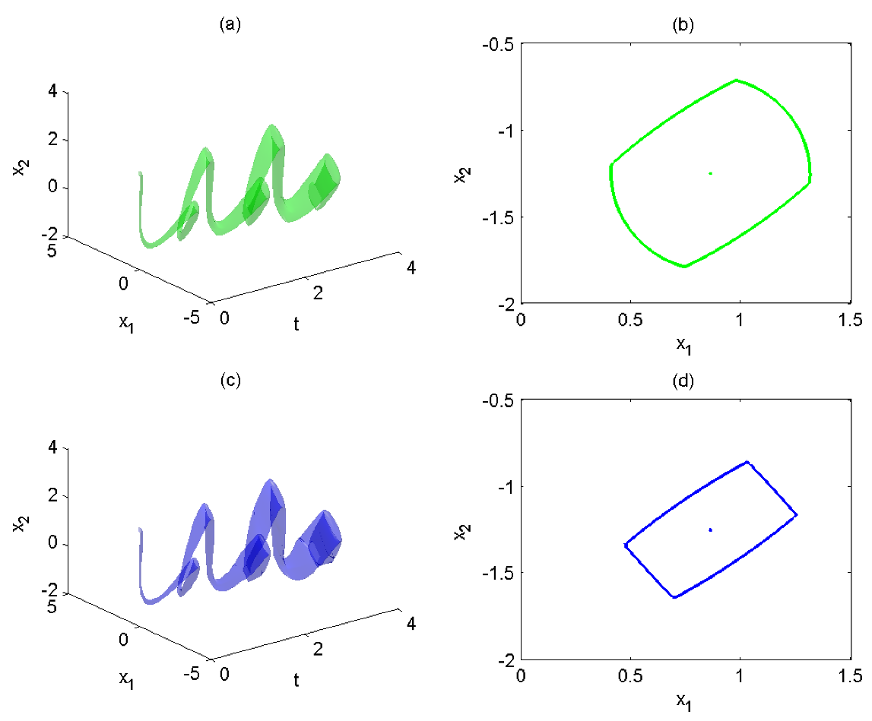
\includegraphics[height=10 cm]{reachmech.eps}}
\caption{Spring-mass system without disturbance:
(a) reach tube for time $t\in[0,4]$; (b) reach set at time $t=4$.
Spring-mass system with disturbance:
(c) reach tube for time $t\in[0,4]$; (d) reach set at time $t=4$.}
\label{mechreachfig}
\end{figure}

So far we considered an ideal system without any disturbance, such as friction.
We introduce disturbance to (\ref{spmass1}-\ref{spmass2}) by adding extra
terms, $v_1$ and $v_2$,
\begin{eqnarray}
m_1\ddot{x}_1+(k_1+k_2)x_1-k_2x_2 & = & u_1 + v_1, \label{smdist1}\\
m_2\ddot{x}_2-k_2x_1+(k_1+k_2)x_2 & = & u_2 + v_2, \label{smdist2}
\end{eqnarray}
which results in equation (\ref{spmassls}) getting an extra term
\[ \left[\begin{array}{cc}
0 & 0\\
0 & 0\\
1 & 0\\
0 & 1\end{array}\right]\left[\begin{array}{c}
v_1\\
v_2\end{array}\right]. \]
Assuming that $[v_1 ~~ v_2]^T$ is unknown but bounded by ellipsoid
$\EE(0, \frac{1}{4}I)$, we can compute the closed-loop reach set of the system
with disturbance.
\verbmcodef[Computation of the closed-loop reach set]
{mcodesnippets/s_chapter06_section02_snippet02.m}

Figure \ref{mechreachfig}(c) shows the reach set of the system
(\ref{smdist1}-\ref{smdist2}) evolving in time from $t=0$ to $t=4$.
Figure \ref{mechreachfig}(d) presents a snapshot of this reach set at time
$t=4$.



\section{Switched System}
By {\it switched systems} we mean systems whose dynamics
changes at known times. Consider the RLC circuit shown in figure \ref{rlcfig}.
It has two inputs - the voltage ($v$) and current ($i$) sources.
Define
\begin{itemize}
\item $x_1$ - voltage across capacitor $C_1$, so $C_1\dot{x}_1$ is
the corresponding current;
\item $x_2$ - voltage across capacitor $C_2$, so the corresponding
current is $C_2\dot{x}_2$.
\item $x_3$ - current through the inductor $L$, so the voltage across
the inductor is $L\dot{x}_3$.
\end{itemize}
\begin{figure}[htbp]
\centerline{
\includegraphics[height=5 cm]{rlc.eps}}
\caption{RLC circuit with two inputs.}
\label{rlcfig}
\end{figure}
Applying Kirchoff current and voltage laws we arrive at the linear system,
\begin{equation}
\left[\begin{array}{c}
\dot{x}_1\\
\dot{x}_2\\
\dot{x}_3\end{array}\right] = \left[\begin{array}{ccc}
-\frac{1}{R_1C_1} & 0 & -\frac{1}{C_1}\\
0 & 0 & \frac{1}{C_2}\\
\frac{1}{L} & -\frac{1}{L} & -\frac{R_2}{L}\end{array}\right]
\left[\begin{array}{c}
x_1\\
x_2\\
x_3\end{array}\right] + \left[\begin{array}{cc}
\frac{1}{R_1C_1} & \frac{1}{C_1}\\
0 & 0\\
0 & 0\end{array}\right]\left[\begin{array}{c}
v\\
i\end{array}\right]. \label{rlceq}
\end{equation}
The parameters $R_1$, $R_2$, $C_1$, $C_2$ and $L$, as well as the inputs,
may depend on time. Suppose, for time $0\leq t<2$, $R_1=2$ Ohm, $R_2=1$ Ohm,
$C_1=3$ F, $C_2=7$ F, $L=2$ H, both inputs, $v$ and $i$ are present and
bounded by ellipsoid $\EE(0,I)$; and for time $t\geq 2$,
$R_1=R_2=2$ Ohm, $C_1=C_2=3$ F, $L=6$ H, the current source is turned off,
and $|v|\leq 1$. Then, system (\ref{rlceq}) can be rewritten as
\begin{equation}
\left[\begin{array}{c}
\dot{x}_1\\
\dot{x}_2\\
\dot{x}_3\end{array}\right] = \left\{\begin{array}{ll}
\left[\begin{array}{ccc}
-\frac{1}{6} & 0 & -\frac{1}{3}\\
0 & 0 & \frac{1}{7}\\
\frac{1}{2} & -\frac{1}{2} & -\frac{1}{2}\end{array}\right]
\left[\begin{array}{c}
x_1\\
x_2\\
x_3\end{array}\right] + \left[\begin{array}{cc}
\frac{1}{6} & \frac{1}{3}\\
0 & 0\\
0 & 0\end{array}\right]\left[\begin{array}{c}
v\\
i\end{array}\right], & 0\leq t< 2, \\
\left[\begin{array}{ccc}
-\frac{1}{6} & 0 & -\frac{1}{3}\\
0 & 0 & \frac{1}{3}\\
\frac{1}{6} & -\frac{1}{6} & -\frac{1}{3}\end{array}\right]
\left[\begin{array}{c}
x_1\\
x_2\\
x_3\end{array}\right] + \left[\begin{array}{c}
\frac{1}{6} \\
0 \\
0 \end{array}\right]v, & 2\leq t. \end{array}\right.
\label{rlceq2}
\end{equation}
We can compute the reach set of (\ref{rlceq2}) for some time $t>2$, say, $t=3$.

\verbmcodef[Computation of the reach set for time interval]
{mcodesnippets/s_chapter06_section03_snippet01.m}

Figure \ref{rlcreachfig}(a) shows how the reach set projection
onto $(x_1, x_2)$ of system (\ref{rlceq2})
evolves in time from $t=0$  to $t=3$. The external reach set approximation
for the first dynamics is in red, the internal approximation is in green.
The dynamics switches at $t=2$.
The external reach set approximation for the second dynamics is in yellow,
its internal approximation is in blue.
The full three-dimensional external (yellow) and internal (blue)
approximations of the reach set are shown in figure \ref{rlcreachfig}(b).
\begin{figure}[htbp]
\centerline{
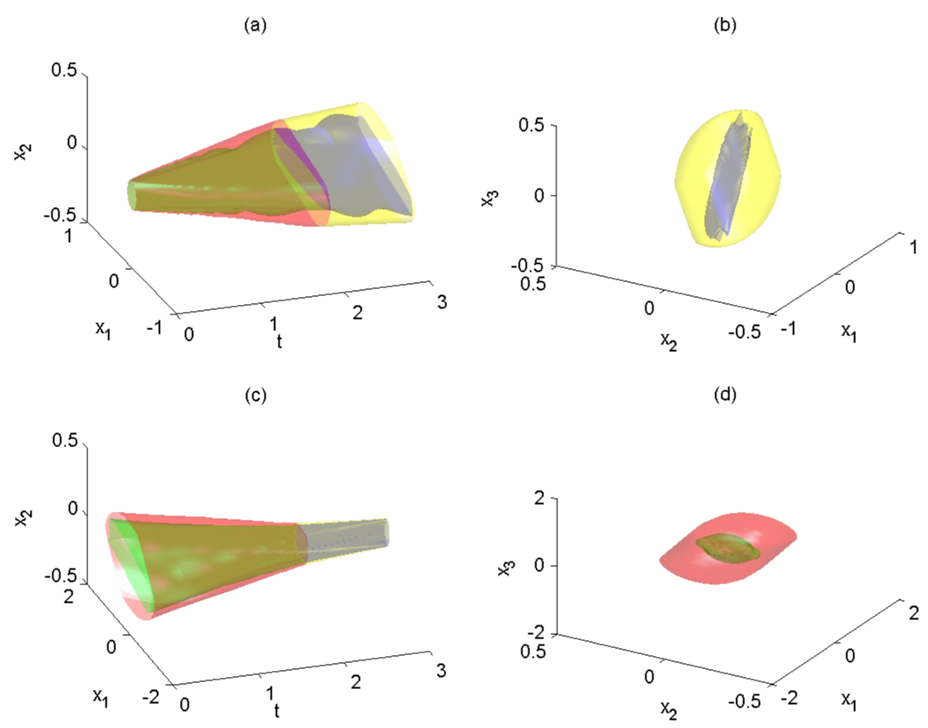
\includegraphics[height=10 cm]{rlcreach.eps}}
\caption{Forward and backward reach sets of the switched system
(external and internal approximations).
The dynamics switches at $t=2$.
\newline
(a) Forward reach set for the time interval $0\leq t\leq3$ projected onto
$(x_1,x_2)$ subspace.
\newline
(b) Forward reach set at $t=3$ in ${\bf R}^3$.
\newline
(c) Backward reach set evolving from $t=3$ to $t=0$ projected onto
$(x_1,x_2)$ subspace.
\newline
(d) Backward reach set at $t=0$ in ${\bf R}^3$.}
\label{rlcreachfig}
\end{figure}

To find out where the system should start at time $t=0$ in order to reach
a neighborhood {\tt M} of the origin at time $t=3$,
we compute the backward reach set from $t=3$ to $t=0$.
\verbmcodef[Computation of the backward reach set]
{mcodesnippets/s_chapter06_section03_snippet02.m}

Figure \ref{rlcreachfig}(c) presents the evolution of the reach set
projection onto $(x_1, x_2)$ in backward time.
Again, external and internal approximations corresponding
to the first dynamics are shown in red and green, and
to the second dynamics in yellow and blue. The
full dimensional backward reach set external and internal
approximations of system (\ref{rlceq2})
at time $t=0$ is shown in figure \ref{rlcreachfig}(d).



\section{Hybrid System}
There is no explicit implementation of the reachability analysis for hybrid
systems in the {\it Ellipsoidal Toolbox}.
Nonetheless, the operations of intersection available in the toolbox allow us
to work with certain class of hybrid systems, namely,
hybrid systems with affine continuous dynamics whose guards are
ellipsoids, hyperplanes, halfspaces or polytopes.

We  consider the {\it switching-mode model} of highway traffic
presented in \cite{xiaotian}. The highway segment is divided into $N$ cells
as shown in figure \ref{hwfig}. In this particular case, $N=4$.
The traffic density in cell $i$ is  $x_i$ vehicles per mile, $i=1,2,3,4$.
\begin{figure}[htbp]
\centerline{
\includegraphics[height=5 cm]{hw.eps}}
\caption{Highway model. Adapted from \cite{xiaotian}.}
\label{hwfig}
\end{figure}

Define
\begin{itemize}
\item $v_i$ - average  speed in mph,
in the $i$-th cell, $i=1,2,3,4$;
\item $w_i$ - backward congestion wave propagation speed in mph,
in the $i$-th highway cell, $i=1,2,3,4$;
\item $x_{Mi}$ - maximum allowed density in the $i$-th cell;
when this velue is reached, there is a traffic jam, $i=1,2,3,4$;
\item $d_i$ - length of $i$-th cell in miles, $i=1,2,3,4$;
\item $T_s$ - sampling time in hours;
\item $b$ - split ratio for the off-ramp;
\item $u_1$ - traffic flow coming into the highway segment,
in vehicles per hour (vph);
\item $u_2$ - traffic flow coming out of the highway segment (vph);
\item $u_3$ - on-ramp traffic flow (vph).
\end{itemize}
Highway traffic operates in two modes: {\it free-flow} in normal operation;
and {\it congested} mode, when there is a jam.
Traffic flow in free-flow mode is described by
\begin{eqnarray}
\left[\begin{array}{c}
x_1[t+1]\\
x_2[t+1]\\
x_3[t+1]\\
x_4[t+1]\end{array}\right] & = & \left[\begin{array}{cccc}
1-\frac{v_1T_s}{d_1} & 0 & 0 & 0\\
\frac{v_1T_s}{d_2} & 1-\frac{v_2T_s}{d_2} & 0 & 0\\
0 & \frac{v_2T_s}{d_3} & 1-\frac{v_3T_s}{d_3} & 0\\
0 & 0 & (1-b)\frac{v_3T_s}{d_4} & 1-\frac{v_4T_s}{d_4}\end{array}\right]
\left[\begin{array}{c}
x_1[t]\\
x_2[t]\\
x_3[t]\\
x_4[t]\end{array}\right] \nonumber\\
& + & \left[\begin{array}{ccc}
\frac{v_1T_s}{d_1} & 0 & 0\\
0 & 0 & \frac{v_2T_s}{d_2}\\
0 & 0 & 0\\
0 & 0 & 0\end{array}\right]\left[\begin{array}{c}
u_1\\
u_2\\
u_3\end{array}\right]. \label{fflow}
\end{eqnarray}
The equation for the congested mode is
\begin{eqnarray}
\left[\begin{array}{c}
x_1[t+1]\\
x_2[t+1]\\
x_3[t+1]\\
x_4[t+1]\end{array}\right] & = & \left[\begin{array}{cccc}
1-\frac{w_1T_s}{d_1} & \frac{w_2T_s}{d_1} & 0 & 0\\
0 & 1-\frac{w_2T_s}{d_2} & \frac{w_3T_s}{d_2} & 0\\
0 & 0 & 1-\frac{w_3T_s}{d_3} & \frac{1}{1-b}\frac{w_4T_s}{d_3}\\
0 & 0 & 0 & 1-\frac{w_4T_s}{d_4}\end{array}\right]
\left[\begin{array}{c}
x_1[t]\\
x_2[t]\\
x_3[t]\\
x_4[t]\end{array}\right] \nonumber\\
& + & \left[\begin{array}{ccc}
0 & 0 & \frac{w_1T_s}{d_1}\\
0 & 0 & 0\\
0 & 0 & 0\\
0 & -\frac{w_4T_s}{d_4} & 0\end{array}\right]\left[\begin{array}{c}
u_1\\
u_2\\
u_3\end{array}\right] \nonumber\\
& + & \left[\begin{array}{cccc}
\frac{w_1T_s}{d_1} & -\frac{w_2T_s}{d_1} & 0 & 0\\
0 & \frac{w_2T_s}{d_2} & -\frac{w_3T_s}{d_2} & 0\\
0 & 0 & \frac{w_3T_s}{d_3} & -\frac{1}{1-b}\frac{w_4T_s}{d_3}\\
0 & 0 & 0 & \frac{w_4T_s}{d_4}\end{array}\right]
\left[\begin{array}{c}
x_{M1}\\
x_{M2}\\
x_{M3}\\
x_{M4}\end{array}\right]. \label{cflow}
\end{eqnarray}
The switch from the free-flow to the congested mode occurs when the density
 $x_2$ reaches $x_{M2}$. In other words, the hyperplane
$H([0 ~ 1 ~ 0 ~ 0]^T, x_{M2})$ is the guard.

We indicate how to implement the reach set computation of this hybrid system.
We first define the two linear systems and the guard.
\verbmcodef[Reach set computation of the hybrid system]
{mcodesnippets/s_chapter06_section04_snippet01.m}

We assume that initially the system is in free-flow mode.
Given a set of initial conditions, we  compute the reach set according
to dynamics (\ref{fflow}) for certain number of time steps.
We will consider the external approximation of the reach set by a single
ellipsoid.
\verbmcodef[Get the external approximation of the reach set by a single
ellipsoid]{mcodesnippets/s_chapter06_section04_snippet02.m}

Having obtained the ellipsoidal array {\tt externalEllMat} representing the reach set
evolving in time, we  determine the  ellipsoids in the array that
intersect the guard.
\verbmcodef[Determination of  the  ellipsoids as an array that intersect the guard]{mcodesnippets/s_chapter06_section04_snippet03.m}

Analyzing the values in array {\tt dVec}, we conclude that the free-flow reach set
has nonempty intersection with hyperplane {\tt grdHyp} at $t=18$
for the first time, and at $t=68$ for the last time.
Between $t=18$ and
$t=68$ it crosses the guard. Figure \ref{hwreachfig}(a) shows the
free-flow reach set projection onto $(x_1,x_2,x_3)$ subspace for $t=10$,
before the guard crossing; figure \ref{hwreachfig}(b) for $t=50$,
during the guard crossing; and figure \ref{hwreachfig}(c) for $t=80$,
after the guard was crossed.
\begin{figure}[htbp]
\centerline{
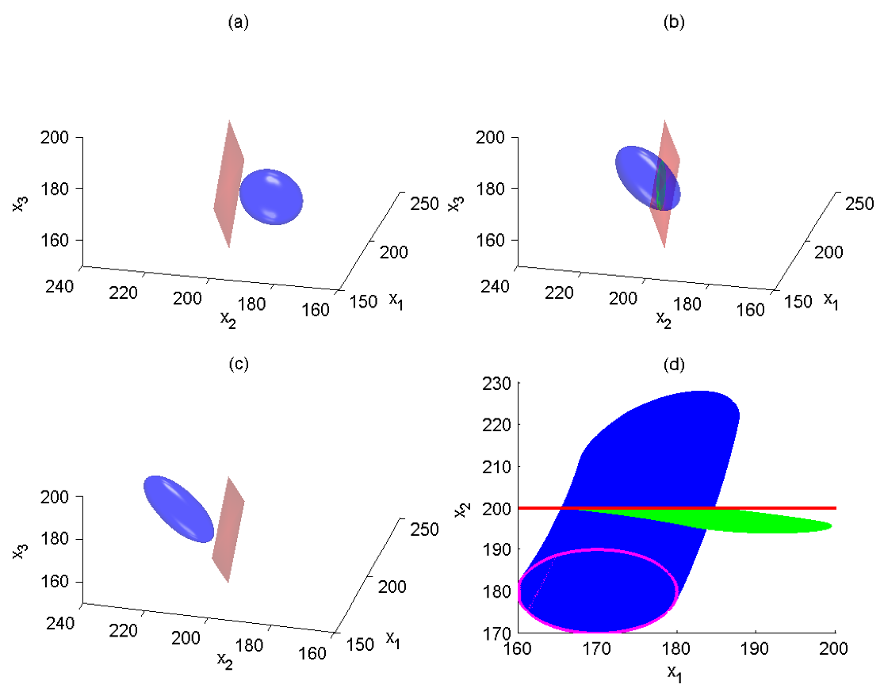
\includegraphics[height=10 cm]{hwreach.eps}}
\caption{Reach set of the free-flow system is blue, reach set of the congested
system is green, the guard is red.
\newline
(a) Reach set of the free-flow system at $t = 10$, before reaching the guard
(projection onto $(x_1,x_2,x_3)$).
\newline
(b) Reach set of the free-flow system at $t = 50$, crossing the guard.
(projection onto $(x_1,x_2,x_3)$).
\newline
(c) Reach set of the free-flow system at $t = 80$, after the guard is crossed.
(projection onto $(x_1,x_2,x_3)$).
\newline
(d) Reach set trace from $t=0$ to $t=100$, free-flow system in blue,
congested system in green; bounds of initial conditions are marked with magenta
(projection onto $(x_1,x_2)$).  }
\label{hwreachfig}
\end{figure}

For each time step that the intersection of the free-flow reach set and the
guard is nonempty, we establish a new initial time and a set of initial
conditions for the reach set computation according to dynamics (\ref{cflow}).
The initial time is the array index minus one, and the set of initial
conditions is the intersection of the free-flow reach set with the guard.
\verbmcodef[The union of reach sets in array]{mcodesnippets/s_chapter06_section04_snippet04.m}

The union of reach sets in array {\tt crs} forms the reach set for
the congested dynamics.

A summary of
 the reach set computation of the
linear hybrid system (\ref{fflow}-\ref{cflow}) for $N=100$ time steps
with one guard crossing is given in figure \ref{hwreachfig}(d),
which shows the projection of the reach set trace onto $(x_1,x_2)$ subspace.
The system starts evolving in time in free-flow mode from a set of
initial conditions at $t=0$, whose boundary is shown in magenta.
The free-flow reach set evolving from $t=0$ to $t=100$ is shown in blue.
Between  $t=18$ and $t=68$ the free-flow reach set crosses the guard.
The guard is shown in red.
For each  nonempty intersection of the free-flow reach set and the guard,
the congested mode reach set starts evolving in time until $t=100$.
All the congested mode reach sets are shown in green.
Observe that in the congested mode, the density $x_2$ in the congested part
 decreases slightly, while the density $x_1$ upstream of the congested part
 increases.
The blue  set above the guard is not actually reached,
because the state evolves according to the green region.


\chapter{Summary and Outlook}\label{ch_summary}
Although some of the operations with ellipsoids are present in the
commercial Geometric Bounding Toolbox \cite{gbt1, gbt2}, the
ellipsoid-related functionality of that toolbox is rather limited.

{\it Ellipsoidal Toolbox} is the first free MATLAB package that
implements ellipsoidal calculus and uses ellipsoidal methods
for reachability analysis of continuous- and discrete-time affine
systems, continuous-time linear systems with disturbances and switched
systems, whose dynamics changes at known times.
The reach set computation for hybrid systems whose guards are hyperplanes
or polyhedra is not implemented explicitly, but the tool for such computation
exists, namely, the operations of intersection of ellipsoid with hyperplane
and ellipsoid with halfspace.




\chapter*{Acknowledgement}
\addcontentsline{toc}{chapter}{Acknowledgement}
The authors would like to thank Alexander B. Kurzhanski,
Manfred Morari, Johan L{\"o}fberg, Michal Kvasnica and Goran Frehse
for their support of this work by useful advice and encouragement.


\bibliographystyle{abbrv}
\bibliography{et}

\appendix
\chapter{Function Reference}\label{appendix_a}
\section{ellipsoid Methods}
{\Large {\tt contains}} -- checks if one ellipsoid contains the other.

Parameters:
\begin{itemize}
\item {\tt E1} -- first ellipsoid or array of ellipsoids.
\item {\tt E2} -- second ellipsoid or array of ellipsoids.
\end{itemize}

Returns $1$ if {\tt E1} contains {\tt E2}, 0 -- otherwise.
\newpage

{\Large {\tt dimension}} - returns the dimension of the space in which
the ellipsoid is defined and the rank of it's shape matrix.

Parameters:
\begin{itemize}
\item {\tt E} -- single ellipsoid or array of ellipsoids.
\end{itemize}

Returns:
\begin{itemize}
\item {\tt n} -- dimension of the space.
\item {\tt r} -- rank of the ellipsoid's shape matrix. This output parameter
is optional.
\end{itemize}

\verbmcodef[Example]{mcodesnippets/s_appendixA_section01_snippet01.m}


\newpage

{\Large {\tt display}} -- displays the details of the ellipsoid object.

Parameters:
\begin{itemize}
\item {\tt E} -- ellipsoid or array of ellipsoids.
\end{itemize}
This function is rarely used explicitely. It is called automatically
for the object {\tt E} when semicolon does not terminate the statement.

\newpage

{\Large {\tt distance}} -- computes the distance from the given ellipsoid
to the specified object -- vector, ellipsoid, hyperplane or polytope.

Parameters:
\begin{itemize}
\item {\tt E} -- ellipsoid or array of ellipsoids.
\item {\tt X} -- in case of vectors, it is a matrix, whose columns represent
the vectors to which the distance is measured, number of columns must match
the number of ellipsoids in the array {\tt E};\\
in case of ellipsoids, it is array of ellipsoids whose size must match the
size of {\tt E};\\
in case of hyperplanes, it is array of hyperplanes whose size must match the
size of {\tt E};\\
in case of polytopes, it is polytope array whose length must match
the number of ellipsoids in the array {\tt E}.
\item {\tt F} - this flag if set to $1$ indicates that the distance should
be computed in the metric of ellipsoids in {\tt E}. This parameter is optional,
its default value is $0$, and the distance is computed in the Euclidean metric.
This parameter makes no difference for the distance computation
between ellipsoids and polytopes.
\end{itemize}

Returns:
\begin{itemize}
\item {\tt D} -- distance or array of distances.
\end{itemize}

\verbmcodef[Example]{mcodesnippets/s_appendixA_section01_snippet02.m}


\newpage

{\Large {\tt double}} -- returns parameters of the ellipsoid, its center
and shape matrix.

Parameters:
\begin{itemize}
\item {\tt E} -- single ellipsoid.
\end{itemize}

Returns:
\begin{itemize}
\item {\tt q} -- center of the ellipsoid. It is optional output parameter.
\item {\tt Q} -- shape matrix of the ellipsoid.
\end{itemize}

\newpage
{\Large {\tt ellintersection\_ia}} -- computes maximum volume ellipsoid that is
contained in the intersection of given ellipsoids.

Parameters:
\begin{itemize}
\item {\tt EL} -- array of ellipsoids of the same dimensions.
\end{itemize}
Returns:
\begin{itemize}
\item {\tt M} -- resulting maximum volume ellipsoid.
\end{itemize}
\newpage
{\Large {\tt ellipsoid}} -- constructor for the ellipsoid object.
If called without parameters, returns empty ellipsoid.

Parameters:
\begin{itemize}
\item {\tt q} -- center of the ellipsoid, vector in ${\bf R}^n$.
This parameter is optional, and if omitted, it is assumed that the ellipsoid
is centered at the origin.
\item {\tt Q} -- shape matrix of the ellipsoid, matrix in ${\bf R}^{n\times n}$,
symmetric positive semidefinite.
\end{itemize}
Returns:
\begin{itemize}
\item {\tt E} -- object of type {\tt ellipsoid class}.
\end{itemize}
\verbmcodef[Example]{mcodesnippets/s_appendixA_section01_snippet03.m}

This example creates a ball of radius $3$ in ${\bf R}^4$ centered at $[1 ~ 0 ~ -1 ~ 6]^T$.

\newpage

{\Large {\tt ellunion\_ea}} -- computes minimum volume ellipsoid that contains union
of given ellipsoids.

Parameters:
\begin{itemize}
\item {\tt EL} -- array of ellipsoids of the same dimensions.
\end{itemize}
Returns:
\begin{itemize}
\item {\tt m} -- resulting minimum volume ellipsoid.
\end{itemize}

\newpage
{\Large {\tt eq}} -- overloaded operator {\tt '=='},
it checks if two ellipsoids are equal.

Parameters:
\begin{itemize}
\item {\tt E1} -- first ellipsoid or array of ellipsoids.
\item {\tt E2} -- second ellipsoid or array of ellipsoids.
\end{itemize}

Returns $1$ if two ellipsoids are equal, $0$ -- otherwise.

\verbmcodef[Example]{mcodesnippets/s_appendixA_section01_snippet04.m}


\newpage

{\Large {\tt ge}}, {\Large {\tt gt}} -- checks if the first ellipsoid is bigger
than the second one.

Parameters:
\begin{itemize}
\item {\tt E1} -- first ellipsoid or array of ellipsoids.
\item {\tt E2} -- second ellipsoid or array of ellipsoids.
\end{itemize}

Returns $1$ if {\tt E1} contains {\tt E2} when both have the same center,
$0$ -- otherwise.

\verbmcodef[Example]{mcodesnippets/s_appendixA_section01_snippet05.m}

This example illustrates the fact that an ellipsoid is always bigger than itself.

\newpage
{\Large {\tt getAbsTol}} -- gives array the same size as input array with values of {\tt absTol} properties for each ellipsoid in input array.

Parameters:
\begin{itemize}
\item {\tt EL} -- array of ellipsoids.
\end{itemize}

Returns:
\begin{itemize}
\item {\tt A} -- array of absTol
properties for ellipsoids in {\tt EL}.
\end{itemize}

\newpage

{\Large {\tt getNPlot2dPoints}} -- gives value of {\tt nPlot2dPoints} property
of ellipsoids in input array of ellipsoids.

Parameters:
\begin{itemize}
\item {\tt EL} -- array of ellipsoids.
\end{itemize}

Returns:
\begin{itemize}
\item {\tt N2} -- array of {\tt nPlot2dPoints} property for ellipsoids
 in {\tt EL}.
\end{itemize}

\newpage

{\Large {\tt getNPlot3dPoints}} -- gives value of {\tt nPlot3dPoints} property
of ellipsoids in input array of ellipsoids.

Parameters:
\begin{itemize}
\item {\tt EL} -- array of ellipsoids.
\end{itemize}

Returns:
\begin{itemize}
\item {\tt N3} -- array of {\tt nPlot2dPoints} property for ellipsoids
 in {\tt EL}.
\end{itemize}

\newpage

{\Large {\tt getRelTol}} -- gives array the same size as input array with values of {\tt relTol}
properties for each ellipsoid in input array.

Parameters:
\begin{itemize}
\item {\tt EL} -- array of ellipsoids.
\end{itemize}

Returns:
\begin{itemize}
\item {\tt R} -- array of {\tt relTol} properties for ellipsoids in EL.
\end{itemize}

\newpage

{\Large {\tt hpintersection}} -- computes the ellipsoid which results from
intersection of given ellipsoid with given hyperplane.

Parameters:
\begin{itemize}
\item {\tt E} -- ellipsoid or array of ellipsoids.
\item {\tt H} -- hyperplane or array of hyperplanes.
\end{itemize}
If {\tt E} and {\tt H} are arrays, then their sizes must match.

Returns:
\begin{itemize}
\item {\tt I} -- ellipsoid or array of ellipsoids that are intersections of
ellipsoids in {\tt E} with hyperplanes in {\tt H}.
\end{itemize}

\verbmcodef[Example]{mcodesnippets/s_appendixA_section01_snippet06.m}


\newpage

{\Large {\tt intersect}} -- checks if the union or intersection of ellipsoids
intersects given ellipsoid, hyperplane or polytope.

Parameters:
\begin{itemize}
\item {\tt E} -- ellipsoid or array of ellipsoids whose union or intersection
is considered.
\item {\tt X} -- can be single or array of ellipsoids, hyperplanes or polytopes.
\item {\tt s} -- if {\tt 'u'}, {\tt E} should be treated as union of ellipsoids,
if {\tt 'i'}, {\tt E} should be treated as intersection of ellipsoids.
This parameter is optional, its default value is {\tt 'u'}.
\end{itemize}

Returns $-1$ in case parameter {\tt s} is set to {\tt 'i'} and the
intersection of ellipsoids in {\tt E} is empty,\\
$0$ if the union or intersection of ellipsoids in {\tt E} does not intersect
the object in {\tt X},\\
$1$ if the union or intersection of ellipsoids in {\tt E} and the object
in {\tt X} have nonempty intersection.

\verbmcodef[Example]{mcodesnippets/s_appendixA_section01_snippet07.m}

Here two ellipsoids {\tt E1} and {\tt E2} do not intersect but both are
intersected by hyperplane {\tt H}.

\newpage

{\Large {\tt intersection\_ea}} -- computes the external ellipsoidal
approximation of the intersection of the ellipsoid with given ellipsoid,
halfspace or polytope.

Parameters:
\begin{itemize}
\item {\tt E} -- ellipsoid or array of ellipsoids.
\item {\tt X} -- can be single or array of ellipsoids, hyperplanes or polytopes.
\end{itemize}
If {\tt E} and {\tt X} are arrays, then their sizes must match.

Returns:
\begin{itemize}
\item {\tt EA} -- ellipsoid or array of ellipsoids that externally approximate
the intersection.
\end{itemize}

\verbmcodef[Example]{mcodesnippets/s_appendixA_section01_snippet08.m}


\newpage

{\Large {\tt intersection\_ia}} -- computes the internal ellipsoidal
approximation of the intersection of the ellipsoid with given ellipsoid,
halfspace or polytope.

Parameters:
\begin{itemize}
\item {\tt E} -- ellipsoid or array of ellipsoids.
\item {\tt X} -- can be single or array of ellipsoids, hyperplanes or polytopes.
\end{itemize}
If {\tt E} and {\tt X} are arrays, then their sizes must match.

Returns:
\begin{itemize}
\item {\tt IA} -- ellipsoid or array of ellipsoids that internally approximate
the intersection.
\end{itemize}

\verbmcodef[Example]{mcodesnippets/s_appendixA_section01_snippet09.m}


\newpage

{\Large {\tt inv}} -- inverts the shape matrix of the ellipsoid if it is
nonsingular.

Parameters:
\begin{itemize}
\item {\tt E} -- ellipsoid or array of ellipsoids.
\end{itemize}

Returns:
\begin{itemize}
\item {\tt I} -- ellipsoid or array of ellipsoids with inverted shape matrices.
\end{itemize}

\newpage

{\Large {\tt isbaddirection}} -- checks if ellipsoidal approximations of
the geometric difference of two ellipsoids can be computed for given
directions.

Parameters:
\begin{itemize}
\item {\tt E1} -- first ellipsoid.
\item {\tt E2} -- second ellipsoid.
\item {\tt L} -- matrix whose columns are direction vectors that need to be
checked.
\end{itemize}

Returns $1$ if given direction is bad and ellipsoidal approximation cannot
be computed for it, $0$ -- otherwise.

\verbmcodef[Example]{mcodesnippets/s_appendixA_section01_snippet10.m}

Means that for vectors $[1 ~ 1]^T$ and $[0 ~ 1]^T$ the ellipsoidal approximation
of the geometric difference ${\tt B}\dot{-}{\tt E}$ cannot be computed.

\newpage

{\Large {\tt isbigger}} -- checks if one ellipsoid would contain the other if their
centers would coincide.

Parameters:
\begin{itemize}
\item {\tt E1} -- first ellipsoid.
\item {\tt E2} -- second ellipsoid.
\end{itemize}

Returns $1$ if ellipsoid {\tt E1}
would contain {\tt E2} inside, 0 -- otherwise.

\newpage

{\Large {\tt isdegenerate}} -- checks if given ellipsoid is degenerate.

Parameters:
\begin{itemize}
\item {\tt E} -- ellipsoid or array of ellipsoids.
\end{itemize}

Returns $1$ if the ellipsoid is degenerate, $0$ -- otherwise.

\newpage

{\Large {\tt isempty}} -- checks if given ellipsoid is an empty object.

Parameters:
\begin{itemize}
\item {\tt E} -- ellipsoid or array of ellipsoids.
\end{itemize}

Returns $1$ if empty, $0$ -- otherwise.

\newpage

{\Large {\tt isinside}} -- checks if the intersection of ellipsoids contains
the union or intersection of given ellipsoids or polytopes.

Parameters:
\begin{itemize}
\item {\tt E} -- ellipsoid or array of ellipsoids whose intersection contains
or not the union or intersection of other given objects.
\item {\tt X} -- can be array of ellipsoids or polytopes whose union or
intersection belongs or not to the intersection {\tt E}.
\item {\tt s} -- if {\tt 'u'}, {\tt X} should be treated as union,
if {\tt 'i'}, {\tt X} should be treated as intersection. This parameter
is optional, its default value is {\tt 'u'}.
\end{itemize}

Returns $-1$ if parameter {\tt s} is set to {\tt 'i'} and the intersection
of ellipsoids or polytopes in {\tt X} is empty,\\
$0$ -- if the intersection {\tt E} does not cover {\tt X},\\
$1$ -- if {\tt E} contains {\tt X}.

\verbmcodef[Example]{mcodesnippets/s_appendixA_section01_snippet11.m}

This example illustrates the fact that any ellipsoid contains its intersection with
another ellipsoid.

\newpage

{\Large {\tt isinternal}} -- checks if the union or intersection of ellipsoids
contains given vectors.

Parameters:
\begin{itemize}
\item {\tt E} -- ellipsoid or array of ellipsoids whose intersection contains
or not given vectors or polytopes.
\item {\tt X} -- can be matrix whose columns represent vectors to be checked.
\item {\tt s} -- if {\tt 'u'}, {\tt E} should be treated as union,
if {\tt 'i'}, {\tt E} should be treated as intersection. This parameter
is optional, its default value is {\tt 'u'}.
\end{itemize}

Returns $1$ if vector in {\tt X} belongs to union or intersection {\tt E},
$0$ -- otherwise.

\verbmcodef[Example]{mcodesnippets/s_appendixA_section01_snippet12.m}


Here the intersection of {\tt E1} and {\tt E2} is empty, and thus, cannot
contain any points. The union, on the other hand, contains centers
of both ellipsoids.

\newpage

{\Large {\tt le}}, {\Large {\tt lt}} -- checks if the second ellipsoid is bigger
than the first one.

Parameters:
\begin{itemize}
\item {\tt E1} -- first ellipsoid or array of ellipsoids.
\item {\tt E2} -- second ellipsoid or array of ellipsoids.
\end{itemize}

Returns $1$ if {\tt E2} contains {\tt E1} when both have the same center,
$0$ -- otherwise.

This operation is the mirror of {\tt ge}, {\tt gt}.

\newpage

{\Large {\tt maxeig}} -- returns the biggest eigenvalue of the ellipsoid.

Parameters:
\begin{itemize}
\item {\tt E} -- ellipsoid or array of ellipsoids.
\end{itemize}

Returns:
\begin{itemize}
\item {\tt a} -- largest eigenvalue or array of largest eigenvalues of
ellipsoids in {\tt E}.
\end{itemize}

\newpage

{\Large {\tt mineig}} -- returns the smallest eigenvalue of the ellipsoid.

Parameters:
\begin{itemize}
\item {\tt E} -- ellipsoid or array of ellipsoids.
\end{itemize}

Returns:
\begin{itemize}
\item {\tt a} -- smallest eigenvalue or array of smallest eigenvalues of
ellipsoids in {\tt E}.
\end{itemize}

\newpage

{\Large {\tt minkdiff}} -- computes and plots the geometric difference of
two ellipsoids in 2D and 3D.

Parameters:
\begin{itemize}
\item {\tt E1} -- first ellipsoid.
\item {\tt E2} -- second ellipsoid.
\item {\tt o} -- options structure whose fields describe how the geometric
difference must be plotted. The fields of this structure are
\begin{itemize}
\item {\tt show\_all} -- if set to $1$, also displays the ellipsoids
{\tt E1} and {\tt E2};
\item {\tt newfigure} -- if set to $1$, each plot command will open a new
figure window;
\item {\tt fill} -- if set to $1$, the resulting set and the ellipsoids,
if plotted in 2D, will be filled with color;
\item {\tt color} -- specifies the color of the plot in the RGB format:
{\tt [x y z]};
\item {\tt shade} -- the level of transparency for 3D plots, takes values
between $0$ and $1$ ($0$ - transparent, $1$ - opaque).
\end{itemize}
This parameter is optional.
\end{itemize}

Returns:
\begin{itemize}
\item {\tt x} -- center of the resulting set.
\item {\tt X} -- matrix whose columns represent the boundary points of the
resulting set. The number of points is defined by parameters
{\tt plot2d\_grid} for 2D plots and {\tt plot3d\_grid} for 3D plots of the
global {\tt ellOptions} structure.
\end{itemize}
Both output parameters are optional.

\newpage

{\Large {\tt minkdiff\_ea}} -- computes external ellipsoidal approximations
of the geometric difference of two ellipsoids of arbitrary dimension
for given directions, if these directions are not bad.

Parameters:
\begin{itemize}
\item {\tt E1} -- first ellipsoid.
\item {\tt E2} -- second ellipsoid.
\item {\tt L} -- matrix whose columns specify the directions for which
the approximations should be computed.
\end{itemize}

Returns:
\begin{itemize}
\item {\tt EA} -- array of computed external ellipsoids. Can be empty, if
all the directions specified in {\tt L} are bad.
\end{itemize}

\verbmcodef[Example]{mcodesnippets/s_appendixA_section01_snippet13.m}

The resulting array {\tt EA} contains only two ellipsoids because two
of the four directions specified in {\tt L} are bad.

\newpage

{\Large {\tt minkdiff\_ia}} -- computes internal ellipsoidal approximations
of the geometric difference of two ellipsoids of arbitrary dimension
for given directions, if these directions are not bad.

Parameters:
\begin{itemize}
\item {\tt E1} -- first ellipsoid.
\item {\tt E2} -- second ellipsoid.
\item {\tt L} -- matrix whose columns specify the directions for which
the approximations should be computed.
\end{itemize}

Returns:
\begin{itemize}
\item {\tt EA} -- array of computed internal ellipsoids. Can be empty, if
all the directions specified in {\tt L} are bad.
\end{itemize}

\verbmcodef[Example]{mcodesnippets/s_appendixA_section01_snippet14.m}

The resulting array {\tt IA} contains only two ellipsoids because two
of the four directions specified in {\tt L} are bad.

\newpage

{\Large {\tt minkmp}} -- computes and plots geometric (Minkowski) sum of the
geometric difference of two ellipsoids and the geometric sum of $n$ ellipsoids
in 2D or 3D.

Parameters:
\begin{itemize}
\item {\tt E1} -- first ellipsoid.
\item {\tt E2} -- second ellipsoid.
\item {\tt EE} -- array of ellipsoids whose geometric sum needs to be computed.
\item {\tt o} -- options structure whose fields describe how the geometric
difference must be plotted. The fields of this structure are
\begin{itemize}
\item {\tt show\_all} -- if set to $1$, also displays the ellipsoids
{\tt E1} and {\tt E2};
\item {\tt newfigure} -- if set to $1$, each plot command will open a new
figure window;
\item {\tt fill} -- if set to $1$, the resulting set and the ellipsoids,
if plotted in 2D, will be filled with color;
\item {\tt color} -- specifies the color of the plot in the RGB format:
{\tt [x y z]};
\item {\tt shade} -- the level of transparency for 3D plots, takes values
between $0$ and $1$ ($0$ - transparent, $1$ - opaque).
\end{itemize}
This parameter is optional.
\end{itemize}

Returns:
\begin{itemize}
\item {\tt x} -- center of the resulting set.
\item {\tt X} -- matrix whose columns represent the boundary points of the
resulting set. The number of points is defined by parameters
{\tt plot2d\_grid} for 2D plots and {\tt plot3d\_grid} for 3D plots of the
global {\tt ellOptions} structure.
\end{itemize}
Both output parameters are optional.

\newpage

{\Large {\tt minkmp\_ea}} -- computes external ellipsoidal approximations
of the geometric (Minkowski) sum of the geometric difference of two ellipsoids
and the geometric sum of $n$ ellipsoids.

Parameters:
\begin{itemize}
\item {\tt E1} -- first ellipsoid.
\item {\tt E2} -- second ellipsoid.
\item {\tt EE} -- array of ellipsoids whose geometric sum needs to be computed.
\item {\tt L} -- matrix whose columns specify the directions for which
the approximations should be computed.
\end{itemize}

Returns:
\begin{itemize}
\item {\tt EA} -- array of computed external ellipsoids. Can be empty, if
all the directions specified in {\tt L} are bad.
\end{itemize}

\verbmcodef[Example]{mcodesnippets/s_appendixA_section01_snippet15.m}

The resulting array {\tt EA} contains only two ellipsoids because two
of the four directions specified in {\tt L} are bad.

\newpage

{\Large {\tt minkmp\_ia}} -- computes internal ellipsoidal approximations
of the geometric (Minkowski) sum of the geometric difference of two ellipsoids
and the geometric sum of $n$ ellipsoids.

Parameters:
\begin{itemize}
\item {\tt E1} -- first ellipsoid.
\item {\tt E2} -- second ellipsoid.
\item {\tt EE} -- array of ellipsoids whose geometric sum needs to be computed.
\item {\tt L} -- matrix whose columns specify the directions for which
the approximations should be computed.
\end{itemize}

Returns:
\begin{itemize}
\item {\tt IA} -- array of computed internal ellipsoids. Can be empty, if
all the directions specified in {\tt L} are bad.
\end{itemize}

\verbmcodef[Example]{mcodesnippets/s_appendixA_section01_snippet16.m}

The resulting array {\tt IA} contains only two ellipsoids because two
of the four directions specified in {\tt L} are bad.

\newpage

{\Large {\tt minkpm}} -- computes and plots geometric (Minkowski) difference of
the geometric sum of ellipsoids and a single ellipsoid in 2D or 3D.

Parameters:
\begin{itemize}
\item {\tt EE} -- array of ellipsoids whose geometric sum needs to be computed.
\item {\tt E} -- single ellipsoid.
\item {\tt o} -- options structure whose fields describe how the geometric
difference must be plotted. The fields of this structure are
\begin{itemize}
\item {\tt show\_all} -- if set to $1$, also displays the ellipsoids
{\tt E1} and {\tt E2};
\item {\tt newfigure} -- if set to $1$, each plot command will open a new
figure window;
\item {\tt fill} -- if set to $1$, the resulting set and the ellipsoids,
if plotted in 2D, will be filled with color;
\item {\tt color} -- specifies the color of the plot in the RGB format:
{\tt [x y z]};
\item {\tt shade} -- the level of transparency for 3D plots, takes values
between $0$ and $1$ ($0$ - transparent, $1$ - opaque).
\end{itemize}
This parameter is optional.
\end{itemize}

Returns:
\begin{itemize}
\item {\tt x} -- center of the resulting set.
\item {\tt X} -- matrix whose columns represent the boundary points of the
resulting set. The number of points is defined by parameters
{\tt plot2d\_grid} for 2D plots and {\tt plot3d\_grid} for 3D plots of the
global {\tt ellOptions} structure.
\end{itemize}
Both output parameters are optional.

\newpage

{\Large {\tt minkpm\_ea}} -- computes external ellipsoidal approximations
of the geometric (Minkowski) difference of the geometric sum of ellipsoids
and a single ellipsoid.

Parameters:
\begin{itemize}
\item {\tt EE} -- array of ellipsoids whose geometric sum needs to be computed.
\item {\tt E} -- single ellipsoid.
\item {\tt L} -- matrix whose columns specify the directions for which
the approximations should be computed.
\end{itemize}

Returns:
\begin{itemize}
\item {\tt EA} -- array of computed external ellipsoids. Can be empty, if
all the directions specified in {\tt L} are bad.
\end{itemize}

\verbmcodef[Example]{mcodesnippets/s_appendixA_section01_snippet17.m}


\newpage

{\Large {\tt minkpm\_ia}} -- computes internal ellipsoidal approximations
of the geometric (Minkowski) difference of the geometric sum of ellipsoids
and a single ellipsoid.

Parameters:
\begin{itemize}
\item {\tt EE} -- array of ellipsoids whose geometric sum needs to be computed.
\item {\tt E} -- single ellipsoid.
\item {\tt L} -- matrix whose columns specify the directions for which
the approximations should be computed.
\end{itemize}

Returns:
\begin{itemize}
\item {\tt IA} -- array of computed internal ellipsoids. Can be empty, if
all the directions specified in {\tt L} are bad.
\end{itemize}

\verbmcodef[Example]{mcodesnippets/s_appendixA_section01_snippet18.m}

The resulting array {\tt IA} contains only two ellipsoids because two
of the four directions specified in {\tt L} are bad.

\newpage

{\Large {\tt minksum}} -- computes and plots the geometric sum of finite
number of ellipsoids in 2D and 3D.

Parameters:
\begin{itemize}
\item {\tt E} -- array of ellipsoids whose geometric sum needs to be computed.
\item {\tt o} -- options structure whose fields describe how the geometric
sum must be plotted. The fields of this structure are
\begin{itemize}
\item {\tt show\_all} -- if set to $1$, also displays the ellipsoids in the
array {\tt E};
\item {\tt newfigure} -- if set to $1$, each plot command will open a new
figure window;
\item {\tt fill} -- if set to $1$, the resulting set and the ellipsoids,
if plotted in 2D, will be filled with color;
\item {\tt color} -- specifies the color of the plot in the RGB format:
{\tt [x y z]};
\item {\tt shade} -- the level of transparency for 3D plots, takes values
between $0$ and $1$ ($0$ - transparent, $1$ - opaque).
\end{itemize}
This parameter is optional.
\end{itemize}

Returns:
\begin{itemize}
\item {\tt x} -- center of the resulting set.
\item {\tt X} -- matrix whose columns represent the boundary points of the
resulting set. The number of points is defined by parameters
{\tt plot2d\_grid} for 2D plots and {\tt plot3d\_grid} for 3D plots of the
global {\tt ellOptions} structure.
\end{itemize}
Both output parameters are optional.

\newpage

{\Large {\tt minksum\_ea}} -- computes external ellipsoidal approximations
of the geometric sum of finite number of ellipsoids of arbitrary dimension
for given directions.

Parameters:
\begin{itemize}
\item {\tt E} -- array of ellipsoids whose geometric sum needs to be
approximated.
\item {\tt L} -- matrix whose columns specify the directions for which
the approximations should be computed.
\end{itemize}

Returns:
\begin{itemize}
\item {\tt EA} -- array of computed external ellipsoids whose length is the same
as the number of columns of matrix {\tt L}.
\end{itemize}

\verbmcodef[Example]{mcodesnippets/s_appendixA_section01_snippet19.m}


\newpage

{\Large {\tt minksum\_ia}} -- computes internal ellipsoidal approximations
of the geometric sum of finite number of ellipsoids of arbitrary dimension
for given directions.

Parameters:
\begin{itemize}
\item {\tt E} -- array of ellipsoids whose geometric sum needs to be
approximated.
\item {\tt L} -- matrix whose columns specify the directions for which
the approximations should be computed.
\end{itemize}

Returns:
\begin{itemize}
\item {\tt IA} -- array of computed internal ellipsoids whose length is the same
as the number of columns of matrix {\tt L}.
\end{itemize}

\verbmcodef[Example]{mcodesnippets/s_appendixA_section01_snippet20.m}


\newpage

{\Large {\tt minus}} -- overloaded operator {\tt '-'}.

Parameters:
\begin{itemize}
\item {\tt E} -- ellipsoid or array of ellipsoids defined in ${\bf R}^n$.
\item {\tt b} -- vector in ${\bf R}^n$ or matrix in ${\bf R}^{n\times m}$,
where $m$ equals the number of ellipsoids in the array {\tt E}.
\end{itemize}

Returns:
\begin{itemize}
\item {\tt E1} -- ellipsoid or array of ellipsoids with same shapes as {\tt E},
but with centers shifted by vectors in {\tt -b}.
\end{itemize}

\verbmcodef[Example]{mcodesnippets/s_appendixA_section01_snippet21.m}


\newpage

{\Large {\tt move2origin}} -- moves given ellipsoids to the origin.

Parameters:
\begin{itemize}
\item {\tt E} -- ellipsoid or array of ellipsoids.
\end{itemize}

Returns:
\begin{itemize}
\item {\tt O} -- the same ellipsoid or array of ellipsoids as {\tt E},
but all centered at the origin.
\end{itemize}

\verbmcodef[Example]{mcodesnippets/s_appendixA_section01_snippet22.m}


\newpage

{\Large {\tt mtimes}} -- overloaded operator {\tt '*'}.

Parameters:
\begin{itemize}
\item {\tt A} -- scalar, or matrix in ${\bf R}^{m\times n}$.
\item {\tt E} -- ellipsoid or array of ellipsoids defined in ${\bf R}^n$.
\end{itemize}

Returns:
\begin{itemize}
\item {\tt E1} -- ellipsoid or array of ellipsoids resulting from linear
transformation of {\tt E}.
\end{itemize}

\verbmcodef[Example]{mcodesnippets/s_appendixA_section01_snippet23.m}


\newpage

{\Large {\tt ne}} -- overloaded operator {\tt '\~{ }='},
it checks if two ellipsoids are not equal.

Parameters:
\begin{itemize}
\item {\tt E1} -- first ellipsoid or array of ellipsoids.
\item {\tt E2} -- second ellipsoid or array of ellipsoids.
\end{itemize}

Returns $1$ if two ellipsoids are not equal, $0$ -- otherwise.

\verbmcodef[Example]{mcodesnippets/s_appendixA_section01_snippet24.m}


\newpage

{\Large {\tt parameters}} -- returns parameters of the ellipsoid, its center
and shape matrix.

Parameters:
\begin{itemize}
\item {\tt E} -- single ellipsoid.
\end{itemize}

Returns:
\begin{itemize}
\item {\tt q} -- center of the ellipsoid. It is optional output parameter.
\item {\tt Q} -- shape matrix of the ellipsoid.
\end{itemize}

{\bf Remark.} This function is obsolete. Use {\tt double} instead.

\newpage

{\Large {\tt plot}} -- plots ellipsoids in 1D, 2D and 3D.

Parameters:
\begin{itemize}
\item {\tt E} -- ellipsoid or array of ellipsoids.
\item {\tt c} -- specifies the color:
\begin{itemize}
\item {\tt 'b'} -- blue;
\item {\tt 'c'} -- cyan;
\item {\tt 'g'} -- green;
\item {\tt 'k'} -- black;
\item {\tt 'm'} -- magenta;
\item {\tt 'r'} -- red;
\item {\tt 'w'} -- white;
\item {\tt 'y'} -- yellow.
\end{itemize}
This parameter is optional.
\item {\tt o} -- options structure whose fields describe how the ellipsoids
must be plotted. The fields of this structure are
\begin{itemize}
\item {\tt newfigure} -- if set to $1$, each plot command will open a new
figure window;
\item {\tt fill} -- if set to $1$, the resulting set and the ellipsoids,
if plotted in 2D, will be filled with color;
\item {\tt width} -- specifies line width for 1D and 2D plots;
\item {\tt color} -- specifies the color of the plot in the RGB format:
{\tt [x y z]};
\item {\tt shade} -- the level of transparency for 3D plots, takes values
between $0$ and $1$ ($0$ - transparent, $1$ - opaque).
\end{itemize}
This parameter is optional.
\end{itemize}

Returns: None.

\newpage

{\Large {\tt plus}} -- overloaded operator {\tt '+'}.

Parameters:
\begin{itemize}
\item {\tt E} -- ellipsoid or array of ellipsoids defined in ${\bf R}^n$.
\item {\tt b} -- vector in ${\bf R}^n$ or matrix in ${\bf R}^{n\times m}$,
where $m$ equals the number of ellipsoids in the array {\tt E}.
\end{itemize}

Returns:
\begin{itemize}
\item {\tt E1} -- ellipsoid or array of ellipsoids with same shapes as {\tt E},
but with centers shifted by vectors in {\tt b}.
\end{itemize}

\verbmcodef[Example]{mcodesnippets/s_appendixA_section01_snippet25.m}


\newpage

{\Large {\tt polar}} -- computes polars for ellipsoids which contain the origin.

Parameters:
\begin{itemize}
\item {\tt E} -- ellipsoid or array of ellipsoids.
\end{itemize}

Returns:
\begin{itemize}
\item {\tt P} -- polar ellipsoid or array of polar ellipsoids for those
in {\tt E}.
\end{itemize}

For ellipsoids that do not contain the origin, this function returns empty
ellipsoid.
\verbmcodef[Example]{mcodesnippets/s_appendixA_section01_snippet26.m}

Illustrates the fact that polar set of an ellipsoid centered at the origin
equals to inverse of this ellipsoid.

\newpage

{\Large {\tt projection}} -- computes projection of ellipsoids onto given
orthogonal basis.

Parameters:
\begin{itemize}
\item {\tt E} -- ellipsoid or array of ellipsoids defined in ${\bf R}^n$.
\item {\tt B} -- matrix in ${\bf R}^{n\times m}$ whose columns are orthogonal.
\end{itemize}

Returns:
\begin{itemize}
\item {\tt P} -- array of projected ellipsoids.
\end{itemize}
\verbmcodef[Example]{mcodesnippets/s_appendixA_section01_snippet27.m}


\newpage

{\Large {\tt rho}} -- computes the support function of the ellipsoids for
given directions and corresponding boundary points.

Parameters:
\begin{itemize}
\item {\tt E} -- ellipsoid or array of ellipsoids defined in ${\bf R}^n$.
\item {\tt L} -- vector in ${\bf R}^n$ if {\tt E} is an array of ellipsoids,
otherwise, if {\tt E} is a single ellipsoid, it can be matrix in
${\bf R}^{n\times m}$ whose columns represent the directions for which
the support function needs to be computed.
\end{itemize}

Returns:
\begin{itemize}
\item {\tt R} -- array of support function values.
\item {\tt X} -- matrix whose columns are boundary points corresponding
to the directions in {\tt L}. This output parameter is optional.
\end{itemize}

\newpage

{\Large {\tt shape}} -- has the same functionality as {\tt mtimes} but
modifies only the shape matrix of the ellipsoid leaving its center as is.

Parameters:
\begin{itemize}
\item {\tt A} -- scalar, or matrix in ${\bf R}^{m\times n}$.
\item {\tt E} -- ellipsoid or array of ellipsoids defined in ${\bf R}^n$.
\end{itemize}

Returns:
\begin{itemize}
\item {\tt E1} -- ellipsoid or array of ellipsoids resulting from modification
of the shape matrices of ellipsoids in {\tt E}.
\end{itemize}

\verbmcodef[Example]{mcodesnippets/s_appendixA_section01_snippet28.m}


\newpage

{\Large {\tt trace}} -- computes trace of given ellipsoids.

Parameters:
\begin{itemize}
\item {\tt E} -- ellipsoid or array of ellipsoids.
\end{itemize}

Returns:
\begin{itemize}
\item {\tt T} -- array of trace values whose size matches the size of {\tt E}.
\end{itemize}

\verbmcodef[Example]{mcodesnippets/s_appendixA_section01_snippet29.m}


\newpage


{\Large {\tt uminus}} -- overloaded operation unitary minus.

Parameters:
\begin{itemize}
\item {\tt E} -- ellipsoid or array of ellipsoids.
\end{itemize}

Returns:
\begin{itemize}
\item {\tt E1} -- array of the same ellipsoids as in {\tt E}, whose centers
are multilied by $-1$.
\end{itemize}

\verbmcodef[Example]{mcodesnippets/s_appendixA_section01_snippet30.m}


\newpage

{\Large {\tt volume}} -- computes volume of given ellipsoids.

Parameters:
\begin{itemize}
\item {\tt E} -- ellipsoid or array of ellipsoids.
\end{itemize}

Returns:
\begin{itemize}
\item {\tt V} -- array of volume values whose size matches the size of {\tt E}.
\end{itemize}

\verbmcodef[Example]{mcodesnippets/s_appendixA_section01_snippet31.m}

\newpage

\section{hyperplane Methods}
{\Large {\tt contains}} -- checks if the hyperplanes contain given vectors.

Parameters:
\begin{itemize}
\item {\tt H} -- hyperplane or array of hyperplanes.
\item {\tt X} -- matrix whose columns represent the vectors needed to be checked.
The number of columns must match the number of hyperplanes in {\tt H}.
\end{itemize}

Returns $1$ if the vector in {\tt X} belongs to the hyperplane in {\tt H},
$0$ -- otherwise.

\verbmcodef[Example]{mcodesnippets/s_appendixA_section02_snippet01.m}


\newpage

{\Large {\tt dimension}} -- returns the dimension of the space in which
the hyperplane is defined.

Parameters:
\begin{itemize}
\item {\tt H} -- hyperplane or array of hyperplanes.
\end{itemize}

Returns:
\begin{itemize}
\item {\tt D} -- array of dimension values of the same size as {\tt H}.
\end{itemize}

\verbmcodef[Example]{mcodesnippets/s_appendixA_section02_snippet02.m}


\newpage

{\Large {\tt display}} -- displays the details of the hyperplane object.

Parameters:
\begin{itemize}
\item {\tt H} -- hyperplane or array of hyperplanes.
\end{itemize}
This function is rarely used explicitely. It is called automatically
for the object {\tt H} when semicolon does not terminate the statement.

\newpage

{\Large {\tt double}} -- returns parameters of the hyperplane object,
its normal and scalar.

Parameters:
\begin{itemize}
\item {\tt H} -- hyperplane object.
\end{itemize}

Parameters:
\begin{itemize}
\item {\tt v} - normal vector.
\item {\tt c} - scalar. This output parameter is optional.
\end{itemize}

\newpage

{\Large {\tt eq}} -- overloaded operator {\tt '=='}.
it checks if two hyperplanes are equal.

Parameters:
\begin{itemize}
\item {\tt H1} -- first hyperplane or array of hyperplanes.
\item {\tt H2} -- second hyperplane or array of hyperplanes.
\end{itemize}

Returns $1$ if two hyperplanes are equal, $0$ -- otherwise.

\verbmcodef[Example]{mcodesnippets/s_appendixA_section02_snippet03.m}


\newpage
{\Large {\tt getAbsTol}} -- gives array the same size as input array with values
of {\tt absTol} properties for each hyperplane in input array.

Parameters:
\begin{itemize}
\item {\tt HP} -- multi - dimensional hyperplane array.
\end{itemize}

Returns:
\begin{itemize}
\item {\tt A} -- array of {\tt absTol} properties for hyperplanes in {\tt HP}.
\end{itemize}

\newpage

{\Large {\tt hyperplane}} -- constructor for the hyperplane object.
If called without parameters, returns empty hyperplane.

Parameters:
\begin{itemize}
\item {\tt V} -- vector in ${\bf R}^n$ or matrix in ${\bf R}^{n\times m}$ whose
columns define the normals to the hyperplanes that need to be created.
\item {\tt C} -- scalar value, or, in case {\tt V} has $m$ columns, it can be
array with $m$ values.
\end{itemize}

Returns:
\begin{itemize}
\item {\tt H} -- hyperplane, or, if {\tt V} has more than one column,
array of hyperplanes.
\end{itemize}

\verbmcodef[Example]{mcodesnippets/s_appendixA_section02_snippet04.m}

This example defines three parallel hyperplanes and returns them in the array {\tt H}.

\newpage

{\Large {\tt isempty}} -- checks if the hyperplane object is empty.

Parameters:
\begin{itemize}
\item {\tt H} -- hyperplane or array of hyperplanes.
\end{itemize}

Returns: $1$ if the hyperplane object is empty, $0$ -- otherwise.

\newpage

{\Large {\tt isparallel}} -- checks if the hyperplanes are parallel.

Parameters:
\begin{itemize}
\item {\tt H1} -- first hyperplane or array of hyperplanes.
\item {\tt H2} -- second hyperplane or array of hyperplanes.
\end{itemize}

Returns $1$ if two hyperplanes are equal, $0$ -- otherwise.

\verbmcodef[Example]{mcodesnippets/s_appendixA_section02_snippet05.m}


\newpage

{\Large {\tt ne}} -- overloaded operator {\tt '\~{ }='},
it checks if two hyperplanes are not equal.

Parameters:
\begin{itemize}
\item {\tt H1} -- first hyperplane or array of hyperplanes.
\item {\tt H2} -- second hyperplane or array of hyperplanes.
\end{itemize}

Returns $1$ if two hyperplanes are not equal, $0$ -- otherwise.

\verbmcodef[Example]{mcodesnippets/s_appendixA_section02_snippet06.m}


\newpage

{\Large {\tt parameters}} -- returns parameters of the hyperplane object,
its normal and scalar.

Parameters:
\begin{itemize}
\item {\tt H} -- hyperplane object.
\end{itemize}

Parameters:
\begin{itemize}
\item {\tt v} -- normal vector.
\item {\tt c} -- scalar. This output parameter is optional.
\end{itemize}

{\bf Remark.} This function is obsolete. Use {\tt double} instead.

\newpage

{\Large {\tt plot}} -- plots hyperplanes in 2D and 3D.

Parameters:
\begin{itemize}
\item {\tt H} -- hyperplane or array of hyperplanes.
\item {\tt c} -- specifies the color:
\begin{itemize}
\item {\tt 'b'} -- blue;
\item {\tt 'c'} -- cyan;
\item {\tt 'g'} -- green;
\item {\tt 'k'} -- black;
\item {\tt 'm'} -- magenta;
\item {\tt 'r'} -- red;
\item {\tt 'w'} -- white;
\item {\tt 'y'} -- yellow.
\end{itemize}
This parameter is optional.
\item {\tt o} -- options structure whose fields describe how the hyperplanes
must be plotted. The fields of this structure are
\begin{itemize}
\item {\tt newfigure} -- if set to $1$, each plot command will open a new
figure window;
\item {\tt size} -- length of the line segment in 2D or square diagonal in 3D.
\item {\tt center} -- center of the line segment in 2D or square diagonal in 3D.
\item {\tt width} -- specifies line width for 2D plots;
\item {\tt color} -- specifies the color of the plot in the RGB format:
{\tt [x y z]};
\item {\tt shade} -- the level of transparency for 3D plots, takes values
between $0$ and $1$ ($0$ -- transparent, $1$ -- opaque).
\end{itemize}
This parameter is optional.
\end{itemize}

Returns: None.

\newpage

{\Large {\tt uminus}} -- overloaded operator unitary minus. It does not change
the hyperplane, and affects only the halfspace this hyperplane defines.

Parameters:
\begin{itemize}
\item {\tt H} -- hyperplane or array of hyperplanes.
\end{itemize}

Returns:
\begin{itemize}
\item {\tt H1} -- array of the same hyperplanes as in {\tt H} whose normals and
scalars are multiplied by $-1$.
\end{itemize}

\verbmcodef[Example]{mcodesnippets/s_appendixA_section02_snippet07.m}


\newpage

\section{linsys Methods}
{\Large {\tt dimension}} -- returns dimensions of state, input, output and
disturbance input spaces.

Parameters:
\begin{itemize}
\item {\tt LSYS} -- linear system or array of linear systems.
\end{itemize}

Returns:
\begin{itemize}
\item {\tt N} -- state space dimension.
\item {\tt I} -- dimension of the input space.
\item {\tt O} -- dimension of the output space.
\item {\tt D} -- dimension of the disturbance input space.
\end{itemize}

\newpage

{\Large {\tt display}} -- displays the details of the linear system object.

Parameters:
\begin{itemize}
\item {\tt LSYS} -- linear system or array of linear systems.
\end{itemize}
This function is rarely used explicitely. It is called automatically
for the object {\tt LSYS} when semicolon does not terminate the statement.

\newpage

{\Large {\tt hasdisturbance}} -- checks if given linear system is the system
with disturbance.

Parameters:
\begin{itemize}
\item {\tt LSYS} -- linear system or array of linear systems.
\end{itemize}

Returns $1$ if it is system with disturbance, $0$ -- otherwise.

\newpage

{\Large {\tt hasnoise}} -- checks if given linear system has noise at the
output.

Parameters:
\begin{itemize}
\item {\tt LSYS} -- linear system or array of linear systems.
\end{itemize}

Returns $1$ if it is system with noise, $0$ -- otherwise.

\newpage

{\Large {\tt isdiscrete}} -- checks if given linear system is discrete-time.

Parameters:
\begin{itemize}
\item {\tt LSYS} -- linear system or array of linear systems.
\end{itemize}

Returns $1$ if the system is discrete-time, $0$ -- otherwise.

\newpage

{\Large {\tt isempty}} -- checks if given linear system is an empty object.

Parameters:
\begin{itemize}
\item {\tt LSYS} -- linear system or array of linear systems.
\end{itemize}

Returns $1$ if {\tt LSYS} is an empty object, $0$ -- otherwise.

\newpage

{\Large {\tt islti}} -- checks if given linear system is time invariant.

Parameters:
\begin{itemize}
\item {\tt LSYS} -- linear system or array of linear systems.
\end{itemize}

Returns $1$ if the system is time invariant, $0$ -- otherwise.

\newpage

{\Large {\tt linsys}} -- constructor for the linear system object.
If called without parameters, creates an empty object.

Parameters:
\begin{itemize}
\item {\tt A} -- matrix $A\in{\bf R}^{n\times n}$, can be symbolic if it
depends on time ($t$ - in continuous case, $k$ - in discrete case).
\item {\tt B} -- matrix $B\in{\bf R}^{n\times m}$, can by symbolic if it
depends on time.
\item {\tt U} -- defines control bounds: it can be ellipsoid object with
dimension $m$; or structure with fields {\tt center} - symbolic vector,
and {\tt shape} -- symbolic matrix, if the ellipsoidal bounds depend on time;
or, if the control is fixed, it can be single vector of type {\it double}
or symbolic.
\item {\tt G} -- matrix $G\in{\bf R}^{n\times d}$, can by symbolic if it
depends on time. This parameter is optional.
\item {\tt V} -- defines disturbance bounds: it can be ellipsoid object with
dimension $d$; or structure with fields {\tt center} -- symbolic vector,
and {\tt shape} -- symbolic matrix, if the ellipsoidal bounds depend on time;
or, if the control is fixed, it can be single vector of type {\it double}
or symbolic. This parameter is optional.
\item {\tt C} -- matrix $C\in{\bf R}^{o\times n}$, can by symbolic if it
depends on time. This parameter is optional.
\item {\tt W} -- defines noise bounds: it can be ellipsoid object with
dimension $o$; or structure with fields {\tt center} -- symbolic vector,
and {\tt shape} -- symbolic matrix, if the ellipsoidal bounds depend on time;
or, if the control is fixed, it can be single vector of type {\it double}
or symbolic. This parameter is optional.
\item {\tt s} -- if set to {\tt 'd'}, indicates that the system is discrete-time.
\end{itemize}

Returns:
\begin{itemize}
\item {\tt LSYS} -- linear system object.
\end{itemize}

\verbmcodef[Example]{mcodesnippets/s_appendixA_section03_snippet01.m}


This example defines the following affine discrete-time system:
\begin{eqnarray*}
\left[\begin{array}{c}
x_1[k+1]\\
x_2[k+1]\end{array}\right] & = & \left[\begin{array}{cc}
0 & 1 + \cos(\frac{\pi k}{2})\\
-2 & 0\end{array}\right] + \left[\begin{array}{c}
0\\
1\end{array}\right]u[k] + \left[\begin{array}{c}
\frac{1}{k+1}\\
0\end{array}\right], ~~~ -2\leq u[k]\leq2\\
y[k] & = & [1 ~~ 0]\left[\begin{array}{c}
x_1[k]\\
x_2[k]\end{array}\right], ~~~ k\geq0.
\end{eqnarray*}

\newpage

\section{reach Methods}
{\Large {\tt cut}} -- extracts a segment of the reach tube from the given start
time to the given end time.

Parameters:
\begin{itemize}
\item {\tt RS} -- reach set object.
\item {\tt T} -- time interval of interest in the form {\tt [t1 t2]}.
If {\tt T} is a single scalar, then the reach set for this particular time
value is returned.
\end{itemize}

Returns:
\begin{itemize}
\item {\tt CRS} -- the resulting reach set object.
\end{itemize}

\newpage

{\Large {\tt dimension}} -- returns the dimension of the reach set and
the dimension of the state space for which the reach set was originally
computed.

Parameters:
\begin{itemize}
\item {\tt RS} -- reach set object.
\end{itemize}

Returns:
\begin{itemize}
\item {\tt d} -- dimension of the reach set.
\item {\tt n} -- dimension of the state space for which the reach set was
originally computed. Values of {\tt d} and {\tt n} can be different if
the reach set object is a result of {\tt projection} operation.
This parameter is optional.
\end{itemize}

\newpage

{\Large {\tt display}} -- displays the details of the reach set object.

Parameters:
\begin{itemize}
\item {\tt RS} -- reach set object.
\end{itemize}
This function is rarely used explicitely. It is called automatically
for the object {\tt LSYS} when semicolon does not terminate the statement.

\newpage

{\Large {\tt evolve}} -- computes further evolution in time of the already
existing reach set.

Parameters:
\begin{itemize}
\item {\tt CRS} -- existing reach set.
\item {\tt T} -- new time horizon.
\item {\tt LSYS} -- linear system object that describes new dynamics.
This parameter is optional.
\end{itemize}

Returns:
\begin{itemize}
\item {\tt RS} -- reach set object.
\end{itemize}

\newpage

{\Large {\tt get\_center}} -- returns trajectory of the center of the reach set.

Parameters:
\begin{itemize}
\item {\tt RS} -- reach set object.
\end{itemize}

Returns:
\begin{itemize}
\item {\tt X} -- matrix whose columns represent the position of the center
at times specified in the second output parameter, {\tt T}.
\item {\tt T} -- array of time values at which the trajectory of the reach set
center is evaluated. This output parameter is optional.
\end{itemize}
The number of columns in {\tt X} and values in {\tt T}
is specified by the parameter
{\tt time\_grid} of the {\tt ellOptions} structure.

\newpage

{\Large {\tt get\_directions}} -- returns the trajectories of the direction
vectors for which the ellipsoidal approximations were computed.

Parameters:
\begin{itemize}
\item {\tt RS} -- reach set object.
\end{itemize}

Returns:
\begin{itemize}
\item {\tt X} -- array of cells where each cell represents a trajectory
of the direction vector, for which the ellipsoidal approximations of the
reach set were computed.
\item {\tt T} -- array of time values at which these trajectories
are evaluated. This output parameter is optional.
\end{itemize}
The number of columns in cells of {\tt X} and values in {\tt T} is specified by
the parameter {\tt time\_grid} of the {\tt ellOptions} structure.

\newpage

{\Large {\tt get\_ea}} -- returns array of ellipsoids that represent the
external approximation of the reach set.

Parameters:
\begin{itemize}
\item {\tt RS} -- reach set object.
\end{itemize}

Returns:
\begin{itemize}
\item {\tt E} -- array of ellipsoids that externally approximate the reach set.
The intersection of ellipsoids in the given column of this array is
the external approximation of the reach set at the time spacified by the
corresponding value in the array {\tt T}.
\item {\tt T} -- array of time values at which the approximations
are evaluated. This output parameter is optional.
\end{itemize}
The number of columns in {\tt E} and values in {\tt T} is specified by
the parameter {\tt time\_grid} of the {\tt ellOptions} structure.

\newpage

{\Large {\tt get\_goodcurves}} -- returns the trajectories along which
the ellipsoidal approximations are touching the actual reach set.

Parameters:
\begin{itemize}
\item {\tt RS} -- reach set object.
\end{itemize}

Returns:
\begin{itemize}
\item {\tt X} -- array of cells where each cell represents a good trajectory
along which one of the computed ellipsoidal approximations touches the
reach set.
\item {\tt T} -- array of time values at which the good trajectories
are evaluated. This output parameter is optional.
\end{itemize}
The number of columns in cells of {\tt X} and values in {\tt T} is specified by
the parameter {\tt time\_grid} of the {\tt ellOptions} structure.

\newpage

{\Large {\tt get\_ia}} -- returns array of ellipsoids that represent the
internal approximation of the reach set.

Parameters:
\begin{itemize}
\item {\tt RS} -- reach set object.
\end{itemize}

Returns:
\begin{itemize}
\item {\tt E} -- array of ellipsoids that internally approximate the reach set.
The union of ellipsoids in the given column of this array is
the internal approximation of the reach set at the time specified by the
corresponding value in the array {\tt T}.
\item {\tt T} -- array of time values at which the approximations
are evaluated. This output parameter is optional.
\end{itemize}
The number of columns in {\tt E} and values in {\tt T} is specified by
the parameter {\tt time\_grid} of the {\tt ellOptions} structure.

\newpage

{\Large {\tt get\_system}} -- returns the linear system object for which
the reach set was computed.

Parameters:
\begin{itemize}
\item {\tt RS} -- reach set object.
\end{itemize}

Returns:
\begin{itemize}
\item {\tt LSYS} -- the linear system object, which was used for the reach
set computation.
\end{itemize}

\newpage

{\Large {\tt intersect}} -- checks if the external or internal approximation
of the reach set intersects with given ellipsoids, hyperplanes or
polytopes.

Parameters:
\begin{itemize}
\item {\tt RS} -- reach set object.
\item {\tt X} -- can be array of ellipsoids, hyperplanes or polytopes.
\item {\tt s} -- if set to {\tt 'i'}, indicates that internal approximation
should be checked, if set to {\tt 'e'} -- external. This input parameter
is optional, its default value is {\tt 'e'}.
\end{itemize}

Returns $1$ if the intersection is nonempty, $0$ -- otherwise.

\newpage

{\Large {\tt iscut}} -- checks if the given reach set object resulted
from {\tt cut} operation.

Parameters:
\begin{itemize}
\item {\tt RS} -- reach set object.
\end{itemize}

Returns $1$ if {\tt RS} is a result of {\tt cut} operation, $0$ -- otherwise.

\newpage

{\Large {\tt isempty}} -- checks if the given reach set object is empty.

Parameters:
\begin{itemize}
\item {\tt RS} - reach set object.
\end{itemize}

Returns $1$ if it is an empty object, $0$ -- otherwise.

\newpage

{\Large {\tt isprojection}} -- checks if the given reach set is a result
of {\tt projection} operation.

Parameters:
\begin{itemize}
\item {\tt RS} -- reach set object.
\end{itemize}

Returns $1$ if {\tt RS} is a projection, $0$ -- otherwise.

\newpage

{\Large {\tt plot\_ea}} -- plots external approximation of the reach set
in 2D and 3D.

Parameters:
\begin{itemize}
\item {\tt RS} -- reach set object.
\item {\tt c} -- specifies the color:
\begin{itemize}
\item {\tt 'b'} -- blue;
\item {\tt 'c'} -- cyan;
\item {\tt 'g'} -- green;
\item {\tt 'k'} -- black;
\item {\tt 'm'} -- magenta;
\item {\tt 'r'} -- red;
\item {\tt 'w'} -- white;
\item {\tt 'y'} -- yellow.
\end{itemize}
This parameter is optional.
\item {\tt o} -- options structure whose fields describe how the reach set
must be plotted. The fields of this structure are
\begin{itemize}
\item {\tt width} -- specifies line width for 2D plots;
\item {\tt fill} -- if set to $1$, the set, if plotted in 2D,
will be filled with color;
\item {\tt color} -- specifies the color of the plot in the RGB format:
{\tt [x y z]};
\item {\tt shade} -- the level of transparency for 3D plots, takes values
between $0$ and $1$ ($0$ - transparent, $1$ - opaque).
\end{itemize}
This parameter is optional.
\end{itemize}

Returns: None.

\newpage

{\Large {\tt plot\_ia}} -- plots internal approximation of the reach set
in 2D and 3D.

Parameters:
\begin{itemize}
\item {\tt RS} -- reach set object.
\item {\tt c} -- specifies the color:
\begin{itemize}
\item {\tt 'b'} -- blue;
\item {\tt 'c'} -- cyan;
\item {\tt 'g'} -- green;
\item {\tt 'k'} -- black;
\item {\tt 'm'} -- magenta;
\item {\tt 'r'} -- red;
\item {\tt 'w'} -- white;
\item {\tt 'y'} -- yellow.
\end{itemize}
This parameter is optional.
\item {\tt o} -- options structure whose fields describe how the reach set
must be plotted. The fields of this structure are
\begin{itemize}
\item {\tt width} -- specifies line width for 2D plots;
\item {\tt fill} -- if set to $1$, the set, if plotted in 2D,
will be filled with color;
\item {\tt color} -- specifies the color of the plot in the RGB format:
{\tt [x y z]};
\item {\tt shade} -- the level of transparency for 3D plots, takes values
between $0$ and $1$ ($0$ -- transparent, $1$ -- opaque).
\end{itemize}
This parameter is optional.
\end{itemize}

Returns: None.

\newpage

{\Large {\tt projection}} -- projects the reach set onto the given orthogonal
basis.

Parameters:
\begin{itemize}
\item {\tt RS} -- reach set object with dimension $n$.
\item {\tt B} -- matrix in ${\bf R}^{n\times m}$ whose columns are orthogonal,
they represent the basis vectors.
\end{itemize}

Returns:
\begin{itemize}
\item {\tt PRS} -- reach set object with the projected reach set.
\end{itemize}

\newpage

{\Large {\tt reach}} -- constructor for the reach set object and the main
function that computes the reach set.

Parameters:
\begin{itemize}
\item {\tt LSYS} -- the linear system object with state space dimension $n$.
\item {\tt X0} -- ellipsoid object with dimension $n$, it represents
the set of initial conditions.
\item {\tt L0} -- matrix in ${\bf R}^{n\times m}$ whose columns represent the
directions for which the new approximations need to be computed.
\item {\tt T} -- time interval in the form {\tt [t0 t1]}. If {\tt t1} is
smaller than {\tt t0}, then the backward reach set should be computed.
If {\tt T} is a scalar, then it is assumed that {\tt t0 = 0}.
\item {\tt o} -- options structure with fields
\begin{itemize}
\item {\tt approximation} -- if set to $0$, then only external approximation
is computed, if set to $1$, then only internal approximation is computed,
if set to $2$ (default value), then both approximations are computed.
\item {\tt save\_all} -- if set to $0$ (default value), then the intermediate
calculation data should not be saved, $1$ indicates the opposite.
\item {\tt minmax} -- for discrete-time systems, if set to $0$ (default value),
then maxmin reach set must be computed, $1$ indicates that minmax reach set is
to be computed; for continuous-time systems -- ignored.
\end{itemize}
This parameter is optional.
\end{itemize}

Returns:
\begin{itemize}
\item {\tt RS} -- reach set object.
\end{itemize}

\newpage

{\Large {\tt refine}} -- adds new approximations for the specified directions
to the given reach set object, thus improving the overall approximation.

Parameters:
\begin{itemize}
\item {\tt RS} -- reach set object with dimension $n$. This object must
contain the intermediate calculation data, otherwise, the refinement
is not possible.
\item {\tt L0} -- matrix in ${\bf R}^{n\times m}$ whose columns represent the
directions for which the new approximations need to be computed.
\item {\tt o} -- options structure with fields
\begin{itemize}
\item {\tt approximation} -- if set to $0$, then only external approximation
is computed, if set to $1$, then only internal approximation is computed,
if set to $2$ (default value), then both approximations are computed.
\item {\tt save\_all} -- if set to $0$, then the intermediate calculation
data should not be saved, $1$ (default value) indicates the opposite.
\end{itemize}
This parameter is optional.
\end{itemize}

Returns:
\begin{itemize}
\item {\tt RRS} -- reach set object with refined approximation.
\end{itemize}

\newpage

\section{Miscellaneous Functions}
{\Large {\tt ell\_simdiag}} -- computes the orthogonal transformation matrix
that simultaneously diagonalizes two symmetric matrices.

Parameters:
\begin{itemize}
\item {\tt A} -- symmetric positive definite matrix in ${\bf R}^{n\times n}$.
\item {\tt B} -- symmetric positive semidefinite matrix in ${\bf R}^{n\times n}$.
\end{itemize}

Returns:
\begin{itemize}
\item {\tt T} -- orthogonal matrix in ${\bf R}^{n\times n}$, such that
$TAT^T$ is identity matrix, and $TBT^T$ is diagonal martrix.
\end{itemize}

\newpage

{\Large {\tt ell\_unitball}} -- creates the ellipsoid object that represents
a unit ball of the given dimension.

Parameters:
\begin{itemize}
\item {\tt n} -- dimension of the space in which the unit ball is defined.
\end{itemize}

Returns:
\begin{itemize}
\item {\tt B} -- ellipsoid object with identity shape matrix centered at the
origin.
\end{itemize}

\newpage

{\Large {\tt ell\_valign}} -- computes the orthogonal matrix that aligns two
vectors.

Parameters:
\begin{itemize}
\item {\tt w} -- vector in ${\bf R}^n$.
\item {\tt v} -- vector in ${\bf R}^n$ that needs to be rotated to be parallel
to {\tt w}.
\end{itemize}

Returns:
\begin{itemize}
\item {\tt S} -- orthogonal matrix in ${\bf R}^{n\times n}$, such that
$Sv = \frac{\|v\|_2}{\|w\|_2}w$.
\end{itemize}

\newpage

{\Large {\tt hyperplane2polytope}} -- converts array of hyperplanes of the
same dimension into the polytope object of the Multi-Parametric Toolbox.

Parameters:
\begin{itemize}
\item {\tt H} -- array of hyperplanes, all of which must have the same dimension.
\end{itemize}

Returns:
\begin{itemize}
\item {\tt P} -- polytope object as defined in the Multi-Parametric Toolbox.
\end{itemize}

\newpage

{\Large {\tt polytope2hyperplane}} -- converts the polytope object of the
Multi-Parametric Toolbox into the array of hyperplanes.

Parameters:
\begin{itemize}
\item {\tt P} -- polytope object as defined in the Multi-Parametric Toolbox.
\end{itemize}

Returns:
\begin{itemize}
\item {\tt H} -- array of hyperplanes.
\end{itemize}

\end{document}


